%% Beginning of file 'sample631.tex'
%%
%% Modified 2021 March
%%
%% This is a sample manuscript marked up using the
%% AASTeX v6.31 LaTeX 2e macros.
%%
%% AASTeX is now based on Alexey Vikhlinin's emulateapj.cls 
%% (Copyright 2000-2015).  See the classfile for details.

%% AASTeX requires revtex4-1.cls and other external packages such as
%% latexsym, graphicx, amssymb, longtable, and epsf.  Note that as of 
%% Oct 2020, APS now uses revtex4.2e for its journals but remember that 
%% AASTeX v6+ still uses v4.1. All of these external packages should 
%% already be present in the modern TeX distributions but not always.
%% For example, revtex4.1 seems to be missing in the linux version of
%% TexLive 2020. One should be able to get all packages from www.ctan.org.
%% In particular, revtex v4.1 can be found at 
%% https://www.ctan.org/pkg/revtex4-1.

%% The first piece of markup in an AASTeX v6.x document is the \documentclass
%% command. LaTeX will ignore any data that comes before this command. The 
%% documentclass can take an optional argument to modify the output style.
%% The command below calls the preprint style which will produce a tightly 
%% typeset, one-column, single-spaced document.  It is the default and thus
%% does not need to be explicitly stated.
%%
%% using aastex version 6.3
\documentclass[linenumbers]{aastex631}

%% The default is a single spaced, 10 point font, single spaced article.
%% There are 5 other style options available via an optional argument. They
%% can be invoked like this:
%%
%% \documentclass[arguments]{aastex631}
%% 
%% where the layout options are:
%%
%%  twocolumn   : two text columns, 10 point font, single spaced article.
%%                This is the most compact and represent the final published
%%                derived PDF copy of the accepted manuscript from the publisher
%%  manuscript  : one text column, 12 point font, double spaced article.
%%  preprint    : one text column, 12 point font, single spaced article.  
%%  preprint2   : two text columns, 12 point font, single spaced article.
%%  modern      : a stylish, single text column, 12 point font, article with
%% 		  wider left and right margins. This uses the Daniel
%% 		  Foreman-Mackey and David Hogg design.
%%  RNAAS       : Supresses an abstract. Originally for RNAAS manuscripts 
%%                but now that abstracts are required this is obsolete for
%%                AAS Journals. Authors might need it for other reasons. DO NOT
%%                use \begin{abstract} and \end{abstract} with this style.
%%
%% Note that you can submit to the AAS Journals in any of these 6 styles.
%%
%% There are other optional arguments one can invoke to allow other stylistic
%% actions. The available options are:
%%
%%   astrosymb    : Loads Astrosymb font and define \astrocommands. 
%%   tighten      : Makes baselineskip slightly smaller, only works with 
%%                  the twocolumn substyle.
%%   times        : uses times font instead of the default
%%   linenumbers  : turn on lineno package.
%%   trackchanges : required to see the revision mark up and print its output
%%   longauthor   : Do not use the more compressed footnote style (default) for 
%%                  the author/collaboration/affiliations. Instead print all
%%                  affiliation information after each name. Creates a much 
%%                  longer author list but may be desirable for short 
%%                  author papers.
%% twocolappendix : make 2 column appendix.
%%   anonymous    : Do not show the authors, affiliations and acknowledgments 
%%                  for dual anonymous review.
%%
%% these can be used in any combination, e.g.
%%
%% \documentclass[twocolumn,linenumbers,trackchanges]{aastex631}
%%
%% AASTeX v6.* now includes \hyperref support. While Wehave built in specific
%% defaults into the classfile you can manually override them with the
%% \hypersetup command. For example,
%%
%% \hypersetup{linkcolor=red,citecolor=green,filecolor=cyan,urlcolor=magenta}
%%
%% will change the color of the internal links to red, the links to the
%% bibliography to green, the file links to cyan, and the external links to
%% magenta. Additional information on \hyperref options can be found here:
%% https://www.tug.org/applications/hyperref/manual.html#x1-40003
%%
%% Note that in v6.3 "bookmarks" has been changed to "true" in hyperref
%% to improve the accessibility of the compiled pdf file.
%%
%% If you want to create your own macros, you can do so
%% using \newcommand. Your macros should appear before
%% the \begin{document} command.
%%
%\usepackage{cite}
%\usepackage{natbib}
%\usepackage{ae,aecompl}
%\usepackage{verbatim}
\usepackage{amsmath}	% Advanced maths commands
\usepackage{amssymb}	% Extra maths symbols
\usepackage{upgreek}
%\usepackage{subcaption}
\newcommand{\vdag}{(v)^\dagger}
\newcommand\aastex{AAS\TeX}
\newcommand\latex{La\TeX}
%\bibpunct{(}{)}{;}{a}{}{,}
\newcommand{\fek}{Fe~K$\alpha$}
\newcommand{\xmm}{{\em XMM-Newton}}
\newcommand{\nustar}{{\em NuSTAR }}
\newcommand{\chandra}{{\em Chandra}}
%\newcommand{\swift}{{\em Swift}}
\newcommand{\suzaku}{{\em Suzaku}}
\newcommand{\sax}{{\em BeppoSAX}}
\newcommand{\vla}{{\small VLA}}
\newcommand{\maxi}{{\small \it MAXI}}
\newcommand{\swift}{{\small \it Swift}}
\newcommand{\bat}{{\small {\it Swift}/BAT}}
\newcommand{\xrt}{{\small {\it Swift}/XRT}}
\newcommand{\uvot}{{\small {\it Swift}/UVOT}}
%\texorpdfstring

\usepackage{tikz}
\usetikzlibrary{matrix}

%% Reintroduced the \received and \accepted commands from AASTeX v5.2
%\received{March 1, 2021}
%\revised{April 1, 2021}
%\accepted{\today}

%% Command to document which AAS Journal the manuscript was submitted to.
%% Adds "Submitted to " the argument.
%\submitjournal{PSJ}

%% For manuscript that include authors in collaborations, AASTeX v6.31
%% builds on the \collaboration command to allow greater freedom to 
%% keep the traditional author+affiliation information but only show
%% subsets. The \collaboration command now must appear AFTER the group
%% of authors in the collaboration and it takes TWO arguments. The last
%% is still the collaboration identifier. The text given in this
%% argument is what will be shown in the manuscript. The first argument
%% is the number of author above the \collaboration command to show with
%% the collaboration text. If there are authors that are not part of any
%% collaboration the \nocollaboration command is used. This command takes
%% one argument which is also the number of authors above to show. A
%% dashed line is shown to indicate no collaboration. This example manuscript
%% shows how these commands work to display specific set of authors 
%% on the front page.
%%
%% For manuscript without any need to use \collaboration the 
%% \AuthorCollaborationLimit command from v6.2 can still be used to 
%% show a subset of authors.
%
%\AuthorCollaborationLimit=2
%
%% will only show Schwarz & Muench on the front page of the manuscript
%% (assuming the \collaboration and \nocollaboration commands are
%% commented out).
%%
%% Note that all of the author will be shown in the published article.
%% This feature is meant to be used prior to acceptance to make the
%% front end of a long author article more manageable. Please do not use
%% this functionality for manuscripts with less than 20 authors. Conversely,
%% please do use this when the number of authors exceeds 40.
%%
%% Use \allauthors at the manuscript end to show the full author list.
%% This command should only be used with \AuthorCollaborationLimit is used.

%% The following command can be used to set the latex table counters.  It
%% is needed in this document because it uses a mix of latex tabular and
%% AASTeX deluxetables.  In general it should not be needed.
%\setcounter{table}{1}

%%%%%%%%%%%%%%%%%%%%%%%%%%%%%%%%%%%%%%%%%%%%%%%%%%%%%%%%%%%%%%%%%%%%%%%%%%%%%%%%
%%
%% The following section outlines numerous optional output that
%% can be displayed in the front matter or as running meta-data.
%%
%% If you wish, you may supply running head information, although
%% this information may be modified by the editorial offices.
\shorttitle{{\it WISE} view of CLAGNs}
\shortauthors{Lyu et al.}
%%
%% You can add a light gray and diagonal water-mark to the first page 
%% with this command:
%% \watermark{text}
%% where "text", e.g. DRAFT, is the text to appear.  If the text is 
%% long you can control the water-mark size with:
%% \setwatermarkfontsize{dimension}
%% where dimension is any recognized LaTeX dimension, e.g. pt, in, etc.
%%
%%%%%%%%%%%%%%%%%%%%%%%%%%%%%%%%%%%%%%%%%%%%%%%%%%%%%%%%%%%%%%%%%%%%%%%%%%%%%%%%
\graphicspath{{./}{figures/}}
\graphicspath{{./}{pic/}}
%% This is the end of the preamble.  Indicate the beginning of the
%% manuscript itself with \begin{document}.

\begin{document}

\title{{\it WISE} view of changing-look AGNs: evidence for a transitional stage of AGNs}

%% LaTeX will automatically break titles if they run longer than
%% one line. However, you may use \\ to force a line break if
%% you desire. In v6.31 you can include a footnote in the title.

%% A significant change from earlier AASTEX versions is in the structure for 
%% calling author and affiliations. The change was necessary to implement 
%% auto-indexing of affiliations which prior was a manual process that could 
%% easily be tedious in large author manuscripts.
%%
%% The \author command is the same as before except it now takes an optional
%% argument which is the 16 digit ORCID. The syntax is:
%% \author[xxxx-xxxx-xxxx-xxxx]{Author Name}
%%
%% This will hyperlink the author name to the author's ORCID page. Note that
%% during compilation, LaTeX will do some limited checking of the format of
%% the ID to make sure it is valid. If the "orcid-ID.png" image file is 
%% present or in the LaTeX pathway, the OrcID icon will appear next to
%% the authors name.
%%
%% Use \affiliation for affiliation information. The old \affil is now aliased
%% to \affiliation. AASTeX v6.31 will automatically index these in the header.
%% When a duplicate is found its index will be the same as its previous entry.
%%
%% Note that \altaffilmark and \altaffiltext have been removed and thus 
%% can not be used to document secondary affiliations. If they are used latex
%% will issue a specific error message and quit. Please use multiple 
%% \affiliation calls for to document more than one affiliation.
%%
%% The new \altaffiliation can be used to indicate some secondary information
%% such as fellowships. This command produces a non-numeric footnote that is
%% set away from the numeric \affiliation footnotes.  NOTE that if an
%% \altaffiliation command is used it must come BEFORE the \affiliation call,
%% right after the \author command, in order to place the footnotes in
%% the proper location.
%%
%% Use \email to set provide email addresses. Each \email will appear on its
%% own line so you can put multiple email address in one \email call. A new
%% \correspondingauthor command is available in V6.31 to identify the
%% corresponding author of the manuscript. It is the author's responsibility
%% to make sure this name is also in the author list.
%%
%% While authors can be grouped inside the same \author and \affiliation
%% commands it is better to have a single author for each. This allows for
%% one to exploit all the new benefits and should make book-keeping easier.
%%
%% If done correctly the peer review system will be able to
%% automatically put the author and affiliation information from the manuscript
%% and save the corresponding author the trouble of entering it by hand.

\correspondingauthor{Qingwen Wu}
\email{qwwu@hust.edu.cn}

\author[0000-0001-8879-368X]{Bing Lyu}
\affiliation{School of Physics, Huazhong University of Science and Technology,
1037 Luoyu Road, 
Wuhan, 430074, China \\}
\affiliation{Shanghai Astronomical Observatory, Chinese Academy of Sciences, 80 Nandan Road,
Shanghai, 200030, China}

\author[0000-0003-4773-4987]{Qingwen Wu}
\affiliation{School of Physics, Huazhong University of Science and Technology,
1037 Luoyu Road,
Wuhan, 430074, China \\}

%\affil{Shanghai Astronomical Observatory\\ CAS, Nandan Road 80 \\ Shanghai, 200030, China}
%\nocollaboration
\author[0000-0002-5385-9586]{Zhen Yan}
\affiliation{Shanghai Astronomical Observatory, Chinese Academy of Sciences, 80 Nandan Road,
Shanghai, 200030, China}

\author[0000-0002-3844-9677]{Wenfei Yu}
\affiliation{Shanghai Astronomical Observatory, Chinese Academy of Sciences, 80 Nandan Road,
Shanghai, 200030, China}
%\collaboration{(AAS Journals Data Scientists collaboration)}

\author{Hao Liu}
\affiliation{University of Science and Technology of China,
No.96, JinZhai Road Baohe District, Hefei, Anhui, 230026, China \\}


%% Note that the \and command from previous versions of AASTeX is now
%% depreciated in this version as it is no longer necessary. AASTeX 
%% automatically takes care of all commas and "and"s between authors names.

%% AASTeX 6.31 has the new \collaboration and \nocollaboration commands to
%% provide the collaboration status of a group of authors. These commands 
%% can be used either before or after the list of corresponding authors. The
%% argument for \collaboration is the collaboration identifier. Authors are
%% encouraged to surround collaboration identifiers with ()s. The 
%% \nocollaboration command takes no argument and exists to indicate that
%% the nearby authors are not part of surrounding collaborations.

%% Mark off the abstract in the ``abstract'' environment. 
\begin{abstract}
The discovery of changing-look active galactic nuclei (CLAGNs) with the rapid change of optical broad emission lines (optical CLAGNs) and/or strong variation of line-of-sight column densities (X-ray CLAGNs) challenges the orientation-based AGN unification model. The physical mechanism is unclear for these two types of CLAGNs. We explore mid-infrared (mid-IR) properties for a sample of 57 optical CLAGNs and 13 X-ray CLAGNs based on the {\it Wide-field Infrared Survey Explorer} ({\it WISE}) data. We find that Eddington-scaled mid-IR luminosities of CLAGNs stay just between low-luminosity AGNs (LLAGNs) and luminous QSOs. The CLAGNs show stronger variabilities compared to those of LLAGNs and QSOs. The result supports that the CLAGNs stay in a transitional stage, and they easily suffer the luminosity variation due to the transition of accretion modes with accretion rate at several percent of Eddington ratio. We estimate the mid-IR time lags for 15 bright CLAGNs with strong mid-IR variability, where the tight correlation between the time lag and the bolometric luminosity ($\tau - L$) for CLAGNs roughly follows that found in the luminous QSOs. We don't find evident differences between X-ray CLAGNs and optical CLAGNs based on their mid-IR luminosity. We suggest that the X-ray CLAGNs may be also triggered by variation of accretion rate (e.g., variable disk winds observed at a moderate inclination angle). 

\end{abstract}

%% Keywords should appear after the \end{abstract} command. 
%% The AAS Journals now uses Unified Astronomy Thesaurus concepts:
%% https://astrothesaurus.org
%% You will be asked to selected these concepts during the submission process
%% but this old "keyword" functionality is maintained in case authors want
%% to include these concepts in their preprints.
\keywords{ Active galactic nuclei (16)---Seyfert galaxies (1447)---Quasars (1319)--- LINER galaxies (925)---Reverberation mapping (2019)}

%Active galactic nuclei (16), Seyfert galaxies (1447), Quasars (1319), LINER galaxies (925), Reverberation mapping (2019)

%% From the front matter, We move on to the body of the paper.
%% Sections are demarcated by \section and \subsection, respectively.
%% Observe the use of the LaTeX \label
%% command after the \subsection to give a symbolic KEY to the
%% subsection for cross-referencing in a \ref command.
%% You can use LaTeX's \ref and \label commands to keep track of
%% cross-references to sections, equations, tables, and figures.
%% That way, if you change the order of any elements, LaTeX will
%% automatically renumber them.
%%
%% We recommend that authors also use the natbib \citep
%% and \citet commands to identify citations.  The citations are
%% tied to the reference list via symbolic KEYs. The KEY corresponds
%% to the KEY in the \bibitem in the reference list below. 

\section{Introduction} \label{sec:intro}

Active galactic nuclei (AGNs) are a special class of galaxies characterized by strong variability and high luminosity of non-stellar origin. The accretion onto the central supermassive black hole (SMBH) is widely accepted as the energy source for the AGN activity. The strong emission lines are another typical feature distinguished from the normal galaxies, where the sources with broad lines (1000-20000 $ \rm{km}\, \rm{s}^{-1}$) are called type 1 AGNs. Based on the relative intensity of the broad and narrow components of the Balmer lines, the type 1 AGNs are further classified into several subclasses \citep[e.g., type 1.5, 1.8, and 1.9, see ][]{1976MNRAS.176P..61O,1981ApJ...249..462O}. The sources observed with only narrow lines (e.g., $<$1000 $ \rm{km}\, \rm{s}^{-1}$) are called type 2 AGNs. The broad lines are observed in some type 2 AGNs in polarized light, which suggest that these sources have hidden broad lines \citep[e.g.,][]{1997Natur.385..700H}. In some low-luminosity LINERs, only low ionization emission lines are detected, where these lines are still ionized by the central point-like weak sources \citep[e.g.,][]{2008ARA&A..46..475H}. About 10 percent of AGNs show strong relativistic jets, where the jets start from the vicinity of BHs and can extend far beyond the host galaxy \citep[e.g., Mpc scale,][]{1989AJ.....98.1195K}. 
 

In the last three decades, it was found that the large diversity properties of observed AGN can be explained by a few parameters (e.g., inclination, jet, accretion rate), which is called AGN unification \citep[e.g.,][and references therein]{1993ARA&A..31..473A,2015ARA&A..53..365N}. The first parameter is inclination angle of putative dusty torus. The suppressed multi-waveband continuum and absence of broad emission lines in type 2 AGNs are caused by obscuration of the dust in the torus. The high column density as constrained from X-ray observations and the hidden broad lines in the optical polarization measurements for some type 2 AGNs support this inclination-dependent unification scheme. The second parameter is collimated relativistic radio jets, where these jets are sometimes observed in optical or even in $\gamma$-ray wavebands. Even though the relativistic jets have been observed for several tens of years, the physical reason behind the radio-loud/quiet dichotomy is still an open issue. The third parameter is accretion rate, where different types of accretion modes may exist in the different types of AGNs. For bright AGNs (e.g., QSOs/Seyferts), the big blue bump in optical/UV bands can be well explained by an optically thick and geometrically thin accretion disk \citep[SSD;][]{1973A&A....24..337S}. The SSD may transit to a geometrically thick, advection-dominated accretion flow when the accretion rate is lower than a critical value \citep[ADAF; e.g.,][for a recent review and references therein]{2014ARA&A..52..529Y}, where most of the accretion energy is advected into SMBH rather than radiated away. The ADAF is much hotter than the SSD, which leads to high-energy emission and can explain many typical features in low-luminosity AGNs \citep[LLAGNs,][]{2008ARA&A..46..475H}. Some LLAGNs (e.g., LINERs, FR I radio galaxies, and BL Lacs) lack the broad emission lines and they do not show evident obscuration, which may be caused by absent clouds in the broad-line region (BLR) or central accretion disk does not provide enough ionization photons.  
     

In recent years, it is found that some AGNs, the so-called ``changing-look" AGNs (CLAGNs), show type transitions within a couple of years or even several months. The term ``changing-look" is firstly used to describe the X-ray CLAGNs, which transit from Compton thick (i.e., hydrogen column density, $N_\mathrm{H}> 10^{24}\,\mathrm{cm}^{-2}$) to Compton thin \citep[i.e., $N_\mathrm{H} < 10^{22-23}\,\mathrm{cm}^{-2}$, e.g.,][]{2003MNRAS.342..422M} and vice-visa. This definition has been extended to optical CLAGNs, where broad lines appear/disappear within several years \citep[i.e., transit from type 1 to type 2 and vice-visa, e.g.,][]{2014ApJ...796..134D,2014ApJ...788...48S,2020ApJ...890L..29A,2020ApJ...901....1W}. There has been some systematic search for CLAGNs using multi-epoch optical spectra \citep[e.g.,][]{2018ApJ...862..109Y,2021MNRAS.503.2583S,2021A&A...650A..33P} and the number of CLAGNs is growing. Based on the orientation-unification AGN model, the broad lines and the torus column density will not change within such a short timescale of years or decades.

 
The physical mechanism of CLAGNs is not fully understood. One scenario is that disappearance/appearance of the broad lines and/or variations of obscuration are caused by the obscuring material moving in or out from our line of sight \citep[e.g.,][]{2013MNRAS.436.1615M,2014MNRAS.443.2862A,2015ApJ...815...55R,2018MNRAS.481.2470T,2019ApJ...887...15W}. However, this scenario is challenged by the low $N_\mathrm{H}$ during type transition \citep[e.g.,][]{2016A&A...593L...9H} and roughly unchanged polarization measurements \citep[e.g.,][]{2019sf2a.conf..509M} in many CLAGNs. The ``changing look'' of second scenario is caused by the change of accretion rate, which will lead to the change of ionization luminosity and/or appearance/disappearance of the clouds in BLR. The multi-wavelength and continuum variability in CLAGNs does support this scenario \citep[e.g.,][]{2017ApJ...846L...7S,2018ApJ...864...27S,2018MNRAS.480.3898N}. The strong intrinsic continuum variation is also found in some X-ray CLAGNs with strong $N_\mathrm{H}$ variation, which suggests that the variation of $N_\mathrm{H}$ may be also driven by the change of accretion disk \citep[e.g., disk winds;][]{2021RAA....21..199L}.

In this work, we analyze the mid-IR variability, color, and Eddington ratio for a sample of both X-ray CLAGNs and optical CLAGNs based on the {\it Wide-field Infrared Survey
Explorer} ({\it WISE}) data. We estimate the mid-IR time lags ($\tau$) for 15 bright CLAGNs using multi-epoch optical and mid-IR observations. We use these observations to understand the basic properties of the central engine and possible differences/similarities between the two types of CLAGNs.  We describe the {\it WISE} data and the CLAGN sample in \autoref{sec:sample}. The results of mid-IR variability, color, and luminosity for CLAGNs are shown in \autoref{sec:mir_var_col_lum}. We present the mid-IR dust reverberation mapping analysis and the $\tau$-$L_\mathrm{bol}$ correlation of CLAGNs in \autoref{sec:tau-L}. Conclusion and discussion are presented in \autoref{sec:dis}. Throughout this work, we adopt a flat $\Lambda-$CDM cosmological model with $H_0$=70 km s$^{-1}$ Mpc $^{-1}$, $\Omega_{m}$=0.27, and $\Omega_{\Lambda}=0.73 $.

\section{{\it WISE} Data and CLAGN Sample} \label{sec:sample}
%\subsection{CLAGN sample}
The \textit{WISE} imaged the full sky approximately every six months in four mid-IR bands, centered at 3.4, 4.6, 12, and 22 $\mu$m \citep[referred to as $W1$, $W2$, $W3$, and $W4$, respectively,][]{2010AJ....140.1868W}, which provides an ideal opportunity to explore the infrared properties of CLAGNs. The {\it WISE} surveyed the full sky 1.2 times in the above four bands from 2010 January to September and cryogen for cooling the $W3$ and $W4$ instruments were exhausted. Then it was placed in hibernation on 2011 February 1. On 2013 October 3, it was reactivated (named as \textit{NEOWISE}) with only $W1$ and $W2$ \citep{2014ApJ...792...30M}. We use the \textit{AllWISE} multi-epoch photometry table and \textit{NEOWISE} single exposure (L1b) source table data retrieved from the NASA/IPAC Infrared Science Archive \footnote{\url{https://irsa.ipac.caltech.edu/Missions/wise.html}}. The \textit{AllWISE} and \textit{NEOWISE} data are screened to exclude the possible bad photometric measurements according to the following criteria:\\
(1) Detection from good-quality frame sets\footnote{\url{http://wise2.ipac.caltech.edu/docs/release/neowise/expsup/sec2_3.html}}, with {frame quality score \texttt{qual\_frame}}$>$0, frame image quality score {\texttt{qi\_fact}}$>$0,
South Atlantic Anomaly separation {\texttt{saa\_sep}}$>0$, and Moon masking
flag {\texttt{moon\_masked}}=0.\\ 
(2) $W1$ $<$15 mag and $W2$ $<$13 mag, which approximately correspond to signal-noise-ratio SNR=10.\\
(3) The number of point-spread-function (PSF) components used in profile fitting (\texttt{nb}$<$3), frames are unaffected (\texttt{cc\textunderscore flags}=`0000') and are not actively de-blended \citep[na$=$0; see also][]{2019MNRAS.483.2362R}.

To explore the mid-IR variability properties of CLAGNs, we collect the reported CLAGNs from the literature. To increase the statistical significance on the variability, the sources with at least 20 valid \textit{WISE} data points are considered. Our sample includes 70 sources, which include 57 optical CLAGNs with the disappearance/appearance of broad lines and 13 X-ray CLAGNs with the variation of $N_\mathrm{H}$. It should be noted that 5 CLAGNs show variations of both broad emission lines and X-ray absorption column density (e.g., ESO 362-G18, NGC 2992, NGC 4151, NGC 4395, and NGC 7582). We adopt the BH mass measurements of these CLAGNs from the literature, which are estimated based on kinematics method \citep[e.g.,][]{2003MNRAS.345.1057M}, reverberation mapping (RM) \citep[e.g.,][]{2011MNRAS.410.1877S,2017ApJ...840...97F}, bulge luminosity \citep[$L_\mathrm{bulge}$, e.g.,][]{2006AJ....131.1236D} and velocity dispersion $\sigma_{*}$ of the host galaxy \citep{2002ApJ...574..740T}. The information of the CLAGN sample is listed in \autoref{source}, where the source name, redshift, the type of CLAGNs, BH mass, infrared magnitude, variability, and color are presented.


%\begin{table}
%\newpage
\startlongtable
\begin{deluxetable}{lllllllllllll}
\tablecaption{CLAGN sample with BH mass and \textit{WISE} variability measurements. Sources with at least 20 valid points of \textit{NEOWISE} data are included here. \label{source}}
%\tablewidth{700pt}
\tablewidth{0pt}
\tabletypesize{\scriptsize}
\tablehead{
\colhead{Name} &\colhead{redshift} & \colhead{Type} & \colhead{Ref} & \colhead{log$M_{BH}/M_{\odot}$} & \colhead{Ref} & \colhead{$\sigma_{m W1}$} & \colhead{$<W1>$} & \colhead{$\sigma_{m W2}$} & \colhead{$<W2>$}  & \colhead{$<W1$-$W2>$} & \colhead{$\Delta\,W1$} & \colhead{$\Delta\,W2$} \\
} 
\decimalcolnumbers
\startdata
1H 0419-577 & 0.1040 & X & 1 & 8.6 & 32 & 0.02 & 10.88 & 0.00 & 9.86 & 1.02 & 0.10 & 0.11 \\
2MASS J16171142+0638333 & 0.2291 & O & 2 & 8.0 & 29 & 0.13 & 13.86 & 0.05 & 12.85 & 1.02 & 0.86 & 0.78 \\
2MASS J22053771-0711147 & 0.2950 & O & 2 & 8.0 & 29 & 0.15 & 13.64 & 0.13 & 12.77 & 0.87 & 0.47 & 0.41 \\
2MASX J09381221+0743398 & 0.0220 & O & 3 & 7.5 & 29 & 0.12 & 11.73 & 0.22 & 11.58 & 0.11 & 0.31 & 0.58 \\
2MASX J09483841+4030436 & 0.0468 & O & 3 & 7.5 & 29 & 0.04 & 11.89 & 0.07 & 11.50 & 0.40 & 0.18 & 0.28 \\
3C 390.3 & 0.0561 & O & 4 & 9.3 & 33 & 0.18 & 9.90 & 0.16 & 8.85 & 1.05 & 0.56 & 0.49 \\
ESO 362-G18 & 0.0124 & O & 5 & 7.7 & 34 & 0.09 & 9.88 & 0.09 & 9.27 & 0.60 & 0.29 & 0.33 \\
Fairall 9 & 0.0461 & O & 4 & 8.4 & 35 & 0.06 & 8.99 & 0.03 & 7.99 & 1.00 & 0.25 & 0.16 \\
HE 1136-2304 & 0.0270 & O & 6 & 7.6 & 6 & 0.36 & 10.84 & 0.21 & 10.02 & 0.84 & 0.90 & 0.96 \\
IC 751 & 0.0315 & X & 7 & 8.5 & 7 & 0.03 & 10.76 & 0.00 & 9.95 & 0.82 & 0.06 & 0.10 \\
IRAS 23226-3843 & 0.0359 & O & 8 & 8.2 & 8 & 0.21 & 11.13 & 0.14 & 10.88 & 0.25 & 0.30 & 0.54 \\
Mrk 1018 & 0.0430 & O & 9 & 7.8 & 36 & 0.14 & 10.87 & 0.16 & 10.39 & 0.46 & 0.88 & 1.27 \\
Mrk 530 & 0.0288 & O & 4 & 8.1 & 37 & 0.10 & 8.50 & 0.10 & 7.58 & 0.92 & 0.48 & 0.45 \\
Mrk 590 & 0.0264 & O & 10 & 7.5 & 38 & 0.14 & 10.22 & 0.22 & 9.79 & 0.41 & 0.42 & 0.69 \\
Mrk 6 & 0.0195 & O & 4 & 8.2 & 39 & 0.57 & 8.56 & 0.49 & 7.70 & 0.84 & 1.74 & 1.52 \\
Mrk 609 & 0.0344 & O & 11 & 7.8 & 40 & 0.09 & 10.43 & 0.13 & 9.94 & 0.47 & 0.48 & 0.64 \\
Mrk 926 & 0.0470 & O & 12 & 8.1 & 41 & 0.20 & 9.56 & 0.16 & 8.66 & 0.89 & 0.57 & 0.46 \\
NGC 1097 & 0.0042 & O & 13 & 8.1 & 42 & 0.09 & 8.22 & 0.09 & 8.00 & 0.21 & 0.14 & 0.22 \\
NGC 1365 & 0.0055 & X & 14 & 6.7 & 43 & 0.09 & 7.72 & 0.07 & 7.03 & 0.69 & 0.25 & 0.26 \\
NGC 1566 & 0.0050 & O & 15 & 6.9 & 44 & 0.28 & 8.82 & 0.42 & 8.53 & 0.28 & 1.09 & 1.57 \\
NGC 2617 & 0.0142 & O & 16 & 7.5 & 45 & 0.15 & 10.12 & 0.18 & 9.55 & 0.57 & 0.79 & 1.03 \\
NGC 2992 & 0.0077 & O & 14 & 7.5 & 46 & 0.19 & 8.57 & 0.23 & 7.94 & 0.63 & 0.73 & 1.04 \\
NGC 3065 & 0.0066 & O & 13 & 8.0 & 47 & 0.06 & 9.75 & 0.04 & 9.73 & 0.02 & 0.07 & 0.12 \\
NGC 3516 & 0.0088 & O & 17 & 7.5 & 38 & 0.16 & 8.83 & 0.17 & 8.19 & 0.63 & 0.63 & 0.60 \\
NGC 4051 & 0.0023 & X & 1 & 6.4 & 48 & 0.12 & 8.90 & 0.12 & 8.10 & 0.80 & 0.41 & 0.43 \\
NGC 4151 & 0.0033 & O & 4 & 7.6 & 38 & 0.29 & 7.32 & 0.25 & 6.24 & 1.06 & 1.13 & 0.79 \\
NGC 4388 & 0.0084 & X & 1 & 6.9 & 49 & 0.16 & 9.29 & 0.23 & 8.39 & 0.89 & 0.47 & 0.68 \\
NGC 4395 & 0.0011 & O & 18 & 5.6 & 50 & 0.20 & 12.44 & 0.18 & 11.66 & 0.78 & 0.66 & 0.56 \\
NGC 4507 & 0.0118 & X & 18 & 7.7 & 51 & 0.09 & 8.69 & 0.08 & 7.61 & 1.07 & 0.35 & 0.31 \\
NGC 454 & 0.0122 & X & 1 & 6.2 & 52 & 0.05 & 12.63 & 0.05 & 12.45 & 0.17 & 0.06 & 0.07 \\
NGC 4939 & 0.0104 & X & 19 & 7.5 & 53 & 0.20 & 9.85 & 0.19 & 9.43 & 0.42 & 0.36 & 0.47 \\
NGC 5548 & 0.0172 & O & 20 & 7.5 & 54 & 0.13 & 8.95 & 0.09 & 8.11 & 0.84 & 0.47 & 0.34 \\
NGC 6300 & 0.0037 & X & 21 & 7.0 & 21 & 0.06 & 9.14 & 0.07 & 8.24 & 0.89 & 0.25 & 0.46 \\
NGC 7469 & 0.0163 & X & 20 & 7.3 & 38 & 0.18 & 8.28 & 0.18 & 7.46 & 0.82 & 0.56 & 0.53 \\
NGC 7582 & 0.0053 & O & 4 & 7.7 & 55 & 0.16 & 7.81 & 0.19 & 6.83 & 0.98 & 0.55 & 0.58 \\
NGC 7674 & 0.0290 & X & 22 & 7.6 & 56 & 0.03 & 9.28 & 0.00 & 8.14 & 1.14 & 0.13 & 0.08 \\
PG 1535+547 & 0.0389 & X & 23 & 7.3 & 23 & 0.09 & 9.79 & 0.08 & 8.97 & 0.82 & 0.56 & 0.45 \\
SDSS J030510.60-010431.6       & 0.0450 & O & 24 & 7.3 & 24 & 0.06 & 12.17 & 0.08 & 11.95 & 0.21 & 0.24 & 0.38 \\
SDSS J080020.98+263648.8       & 0.0267 & O & 24 & 7.1 & 24 & 0.21 & 10.09 & 0.24 & 9.33 & 0.75 & 0.80 & 0.88 \\
SDSS J081319.34+460849.5 & 0.0538 & O & 25 & 7.6 & 29 & 0.15 & 12.71 & 0.24 & 12.38 & 0.28 & 0.45 & 0.67 \\
SDSS J081726.41+101210.1 & 0.0458 & O & 26 & 7.5 & 26 & 0.36 & 12.51 & 0.50 & 11.91 & 0.47 & 0.97 & 1.25 \\
SDSS J082323.89+422048.3 & 0.1515 & O & 27 & 8.1 & 27 & 0.08 & 13.59 & 0.09 & 12.90 & 0.69 & 0.57 & 0.82 \\
SDSS J082942.67+415436.9 & 0.1263 & O & 27 & 8.5 & 27 & 0.22 & 11.91 & 0.16 & 11.00 & 0.92 & 0.73 & 0.58 \\
SDSS J090902.35+133019.4 & 0.0499 & O & 25 & 7.3 & 29 & 0.09 & 13.09 & 0.37 & 12.60 & 0.27 & 0.83 & 1.16 \\
SDSS J091531.04+481407.7 & 0.1005 & O & 26 & 7.8 & 57 & 0.13 & 13.25 & 0.15 & 12.73 & 0.50 & 0.65 & 0.86 \\
SDSS J111536.57+054449.7       & 0.0900 & O & 28 & 7.6 & 57 & 0.20 & 13.32 & 0.25 & 12.50 & 0.77 & 1.06 & 1.64 \\
SDSS J113355.93+670107.0 & 0.0397 & O & 26 & 8.2 & 57 & 0.16 & 11.76 & 0.20 & 11.27 & 0.47 & 0.54 & 0.77 \\
SDSS J122550.30+510846.3 & 0.1679 & O & 26 & 8.6 & 57 & 0.08 & 13.01 & 0.12 & 12.29 & 0.72 & 0.65 & 0.73 \\
SDSS J125403.78+491452.8 & 0.0670 & O & 26 & 8.3 & 57 & 0.08 & 12.74 & 0.12 & 12.43 & 0.30 & 0.34 & 0.45 \\
SDSS J131615.95+301552.2       & 0.0492 & O & 24 & 7.1 & 24 & 0.07 & 11.64 & 0.11 & 11.39 & 0.25 & 0.24 & 0.41 \\
SDSS J132457.29+480241.2       & 0.2716 & O & 27 & 8.0 & 29 & 0.09 & 13.64 & 0.01 & 12.87 & 0.77 & 0.30 & 0.23 \\
SDSS J141324.27+530527.0       & 0.4559 & O & 29 & 8.2 & 29 & 0.30 & 13.45 & 0.38 & 12.44 & 0.94 & 1.45 & 1.72 \\
SDSS J153308.02+443208.4 & 0.0367 & O & 26 & 7.6 & 26 & 0.12 & 11.98 & 0.24 & 11.85 & 0.08 & 0.42 & 0.82 \\
SDSS J155440.25+362952.0       & 0.2368 & O & 25 & 8.0 & 25 & 0.07 & 13.73 & 0.01 & 12.91 & 0.82 & 0.84 & 1.24 \\
SDSS J162501.43+241547.3       & 0.0503 & O & 24 & 6.7 & 24 & 0.12 & 12.55 & 0.17 & 12.19 & 0.34 & 0.39 & 0.55 \\
SDSS J163629.66+410222.4       & 0.0474 & O & 24 & 7.0 & 24 & 0.02 & 12.95 & 0.00 & 12.88 & 0.07 & 0.06 & 0.07 \\
SDSS J172322.31+550413.8 & 0.2947 & O & 27 & 8.6 & 27 & 0.11 & 13.45 & 0.16 & 12.58 & 0.83 & 0.30 & 0.28 \\
SDSSJ120447.91+170256.8        & 0.2979 & O & 30 & 8.0 & 30 & 0.21 & 13.88 & 0.14 & 12.70 & 1.21 & 1.03 & 0.70 \\
UGC 3223 & 0.0156 & O & 31 & 8.0 & 31 & 0.08 & 10.82 & 0.14 & 10.59 & 0.21 & 0.25 & 0.46 \\
UGC 4203 & 0.0135 & X & 14 & 6.8 & 43 & 0.03 & 9.96 & 0.02 & 8.60 & 1.36 & 0.14 & 0.09 \\
WISEA J035301.02-062326.2 & 0.0762 & O & 3 & 7.6 & 29 & 0.07 & 13.09 & 0.08 & 12.54 & 0.54 & 0.24 & 0.20 \\
WISEA J084748.28+182440.0 & 0.0848 & O & 3 & 7.7 & 29 & 0.20 & 12.88 & 0.24 & 12.25 & 0.58 & 0.70 & 0.79 \\
WISEA J100323.46+352503.8 & 0.1189 & O & 28 & 8.0 & 57 & 0.30 & 13.27 & 0.29 & 12.44 & 0.81 & 1.14 & 1.33 \\
WISEA J110057.70-005304.4 & 0.3790 & O & 29 & 8.2 & 29 & 0.09 & 13.55 & 0.06 & 12.59 & 0.96 & 0.40 & 0.40 \\
WISEA J113229.14+035729.1 & 0.0909 & O & 28 & 7.9 & 57 & 0.12 & 13.28 & 0.12 & 12.70 & 0.58 & 0.67 & 0.80 \\
WISEA J131930.75+675355.4 & 0.1664 & O & 28 & 7.5 & 57 & 0.08 & 13.61 & 0.07 & 12.85 & 0.76 & 0.25 & 0.33 \\
WISEA J144754.23+283324.1 & 0.1634 & O & 28 & 8.0 & 57 & 0.13 & 12.89 & 0.15 & 12.17 & 0.72 & 0.56 & 0.67 \\
WISEA J154507.52+170950.8 & 0.0483 & O & 29 & 7.4 & 29 & 0.18 & 12.27 & 0.21 & 11.65 & 0.60 & 0.71 & 0.80 \\
WISEA J154529.63+251127.9 & 0.1170 & O & 28 & 8.1 & 57 & 0.14 & 13.18 & 0.17 & 12.56 & 0.60 & 0.52 & 0.58 \\
WISEA J155258.27+273728.5 & 0.0865 & O & 28 & 8.1 & 57 & 0.06 & 13.51 & 0.00 & 12.92 & 0.58 & 0.32 & 0.49 \\
\enddata
%\tablecomments{}
\end{deluxetable}
%\begin{flushleft}
%\hline
Note. The table lists source name, redshift, CLAGN type (``O'' for optical selected CLAGN and ``X'' for X-ray selected CLAGN), mass, references, the variability ($\sigma_m$) of $W1$ and $W2$, the mean magnitude of $W1$ and $W2$, mean color of $W1$-$W2$, maximum magnitude variation ($\Delta\,W1$ and $\Delta\,W2$) of \textit{WISE} data.\\

References. (1)~\citet{2012MNRAS.421.1803M} (2)~\citet{2019ApJ...874....8M} (3)~\citet{2016ApJ...821...33R} (4)~\citet{2019sf2a.conf..509M} (5)~\citet{2018Galax...6...52A} (6)~\citet{2018A&A...619A.168K} (7)~\citet{2016ApJ...820....5R} (8)~\citet{2020A&A...638A..91K} (9)~\citet{2020A&A...644L...5H} (10)~\citet{2020MNRAS.491.4615K} (11)~\citet{2020MNRAS.499.1005W} (12)~\citet{2021IAUS..356..122W} (13)~\citet{2021MNRAS.503.2583S} (14)~\citet{2003MNRAS.342..422M} (15)~\citet{2020MNRAS.498..718O} (16)~\citet{2017OAP....30..117O} (17)~\citet{2021ApJ...909...18F} (18)~\citet{2021MNRAS.507..687J} (19)~\citet{2005MNRAS.356..295G} (20)~\citet{2018ATel11915....1O} (21)~\citet{2020MNRAS.499.5396J} (22)~\citet{2005A&A...442..185B} (23)~\citet{2008A&A...483..137B} (24)~\citet{2020MNRAS.498.3985Y} (25)~\citet{2017ApJ...846L...7S} (26)~\citet{2019ApJ...883...31F} (27)~\citet{2021A&A...650A..33P} (28)~\citet{2018ApJ...862..109Y} (29)~\citet{2020MNRAS.491.4925G} (30)~\citet{2019ApJ...887...15W} (31)~\citet{2020ApJ...901....1W} (32)~\citet{2014A&A...563A..95D} (33)~\citet{2011MNRAS.410.1877S} (34)~\citet{2014MNRAS.443.2862A} (35)~\citet{2017MNRAS.466.1777P} (36)~\citet{2018MNRAS.480.3898N} (37)~\citet{2018MNRAS.478.4214E} (38)~\citet{2013ApJ...773...90G} (39)~\citet{2018MNRAS.481.4542S} (40)~\citet{2010ApJ...720..786L} (41)~\citet{2010A&A...522A..36K} (42)~\citet{2015ApJ...800...63S} (43)~\citet{2017MNRAS.468L..97O} (44)~\citet{2002ApJ...579..530W} (45)~\citet{2019arXiv190904676R} (46)~\citet{2020MNRAS.496.3412M} (47)~\citet{2001ApJ...554..240E} (48)~\citet{2019MNRAS.487..667C} (49)~\citet{2019ApJ...884..106M} (50)~\citet{2005ApJ...632..799P} (51)~\citet{2011AAS...21822816M} (52)~\citet{2009ApJ...690.1322W} (53)~\citet{2017ApJ...850...74K} (54)~\citet{2014MNRAS.445.3073P} (55)~\citet{2018MNRAS.473.5334R} (56)~\citet{2017NatAs...1..727K} (57)~\citet{2021ApJ...907L..21D} 
%\end{flushleft}
%\end{table}



\section{Mid-IR Eddington ratio, variability and color}\label{sec:mir_var_col_lum}
We calculate the mid-IR luminosity for CLAGNs from the \textit{WISE} magnitude, and the distribution of the mid-IR Eddington ratio is presented in the top panel of \autoref{fig:var_ledd_hist}. For comparison, we also include the distributions for a sample of 49 LLAGNs from \citet{2009MNRAS.399..349G} and 732 luminous QSOs from \citet{2007ApJ...667..131G}, where the sources with at least 20 valid \textit{WISE} data points are considered. The average log$L_\mathrm{W1}/L_\mathrm{Edd}$\, are $-2.33$, $-3.46$, and $-1.48$ for CLAGNs, LLAGNs, and QSOs, respectively. It can be found that CLAGNs have a moderate mean Eddington ratio of mid-IR luminosity compared to those of LLAGNs and QSOs. The X-ray CLAGNs show a little bit higher but roughly similar Eddington ratio with optical CLAGNs, where average ratios of log$L_\mathrm{W1}/L_\mathrm{Edd}$\ are $-2.36$ and $-2.18$ respectively (see Table 2).     
 

To estimate the mid-IR variability amplitude of CLAGNs, we firstly calculate the maximum variation magnitude $\Delta\,W1$ and $\Delta\,W2$ for each selected CLAGN. We find that the majority of CLAGNs change more than $0.3$ mag for $\Delta\,W1$ (50/70) and $\Delta\,W2$ (56/70), which include 6 X-ray CLAGNs (NGC 4051, NGC 4388, NGC 4507, NGC 4939, NGC 7469, and PG 1535+547). 

We further calculate the intrinsic variability based on the standard deviation about the mean offset for each CLAGN ($\sigma_m$) following \citet{2019MNRAS.483.2362R} \citep[see also][etc]{2007AJ....134.2236S,2012ApJ...759L..31J}.
The magnitude standard deviation $\Sigma$ is given as
\begin{equation}
\Sigma=\sqrt{\frac{1}{n-1}\sum_{i=1}^{N}(m_i - <m>)^2},
\end{equation}
where $m_i$ is the magnitude at $i$-th point and $<m>$ is the error-weighted average.
The amplitude of variability $\sigma_m$ is  
\[\sigma_m  =
  \begin{cases}
    \sqrt{\Sigma^2 - \epsilon^2},  & \quad \text{if } \Sigma>\epsilon,\\
     0,                            & \quad  \text{otherwise.}\\
  \end{cases}
\]	               
where the error $\epsilon$ is calculated from the individual errors as
\begin{equation}
\epsilon^2=\frac{1}{N}\sum_{i=i}^{N}{\epsilon_{i}^{2} + \epsilon_{s}^2}, 
\end{equation}
where $\epsilon_{i}$ is the measurement uncertainty of $i$-th point and $\epsilon_{s}$ is the systematic uncertainty. The systematic uncertainties for $W1$ and $W2$ are 0.024 mag and 0.028 mag \citep{2011ApJ...735..112J}, respectively. We find that the majority of CLAGNs show strong mid-IR variability with $\sigma_{m \rm{W1}}$ (41/70)  and $\sigma_{m \rm{W2}}$ (44/70) greater than 0.1 mag, and 4 of them are X-ray CLAGNs (NGC 4051, NGC 4388, NGC 4939, and NGC 7469). In \autoref{fig:var_ledd_hist}, we present the correlation between the variability and the mid-IR Eddington ratio and their distributions. It can be found that the average mid-IR variability is almost two times stronger in CLAGNs than that in both LLAGNs and QSOs, where average values of $\sigma_{m \rm{W1}}$ are 0.14, 0.08, and 0.09 for CLAGNs, LLAGNs, and QSOs, respectively.  


We calculate the average color $<W1-W2>$ of CLAGNs and also the sample (LLAGNs and QSOs) for comparison. We present the color distribution of $W1$-$W2$ and the correlation between the color and the mid-IR luminosity Eddington ratio in \autoref{fig:color_ledd}. The sources with higher Eddington ratios normally have higher values of $W1$-$W2$. The color $W1$-$W2$ varies from 0 to around 1.4 for CLAGNs with an average value of 0.65, while the average values are 0.08 and 0.83 for LLAGNs and QSOs respectively. The color of brighter/fainter CLAGNs is similar to the QSOs/LLAGNs, respectively (see \autoref{fig:color_ledd}). 
%The $W2$ band shares similar properties with the $W1$ band, and the results are listed in \autoref{table_MIR_var_cor_lum}. 




\begin{figure}
\centering
	% To include a figure from a file named example.*
	% Allowable file formats are eps or ps if compiling using latex
	% or pdf, png, jpg if compiling using pdflatex
	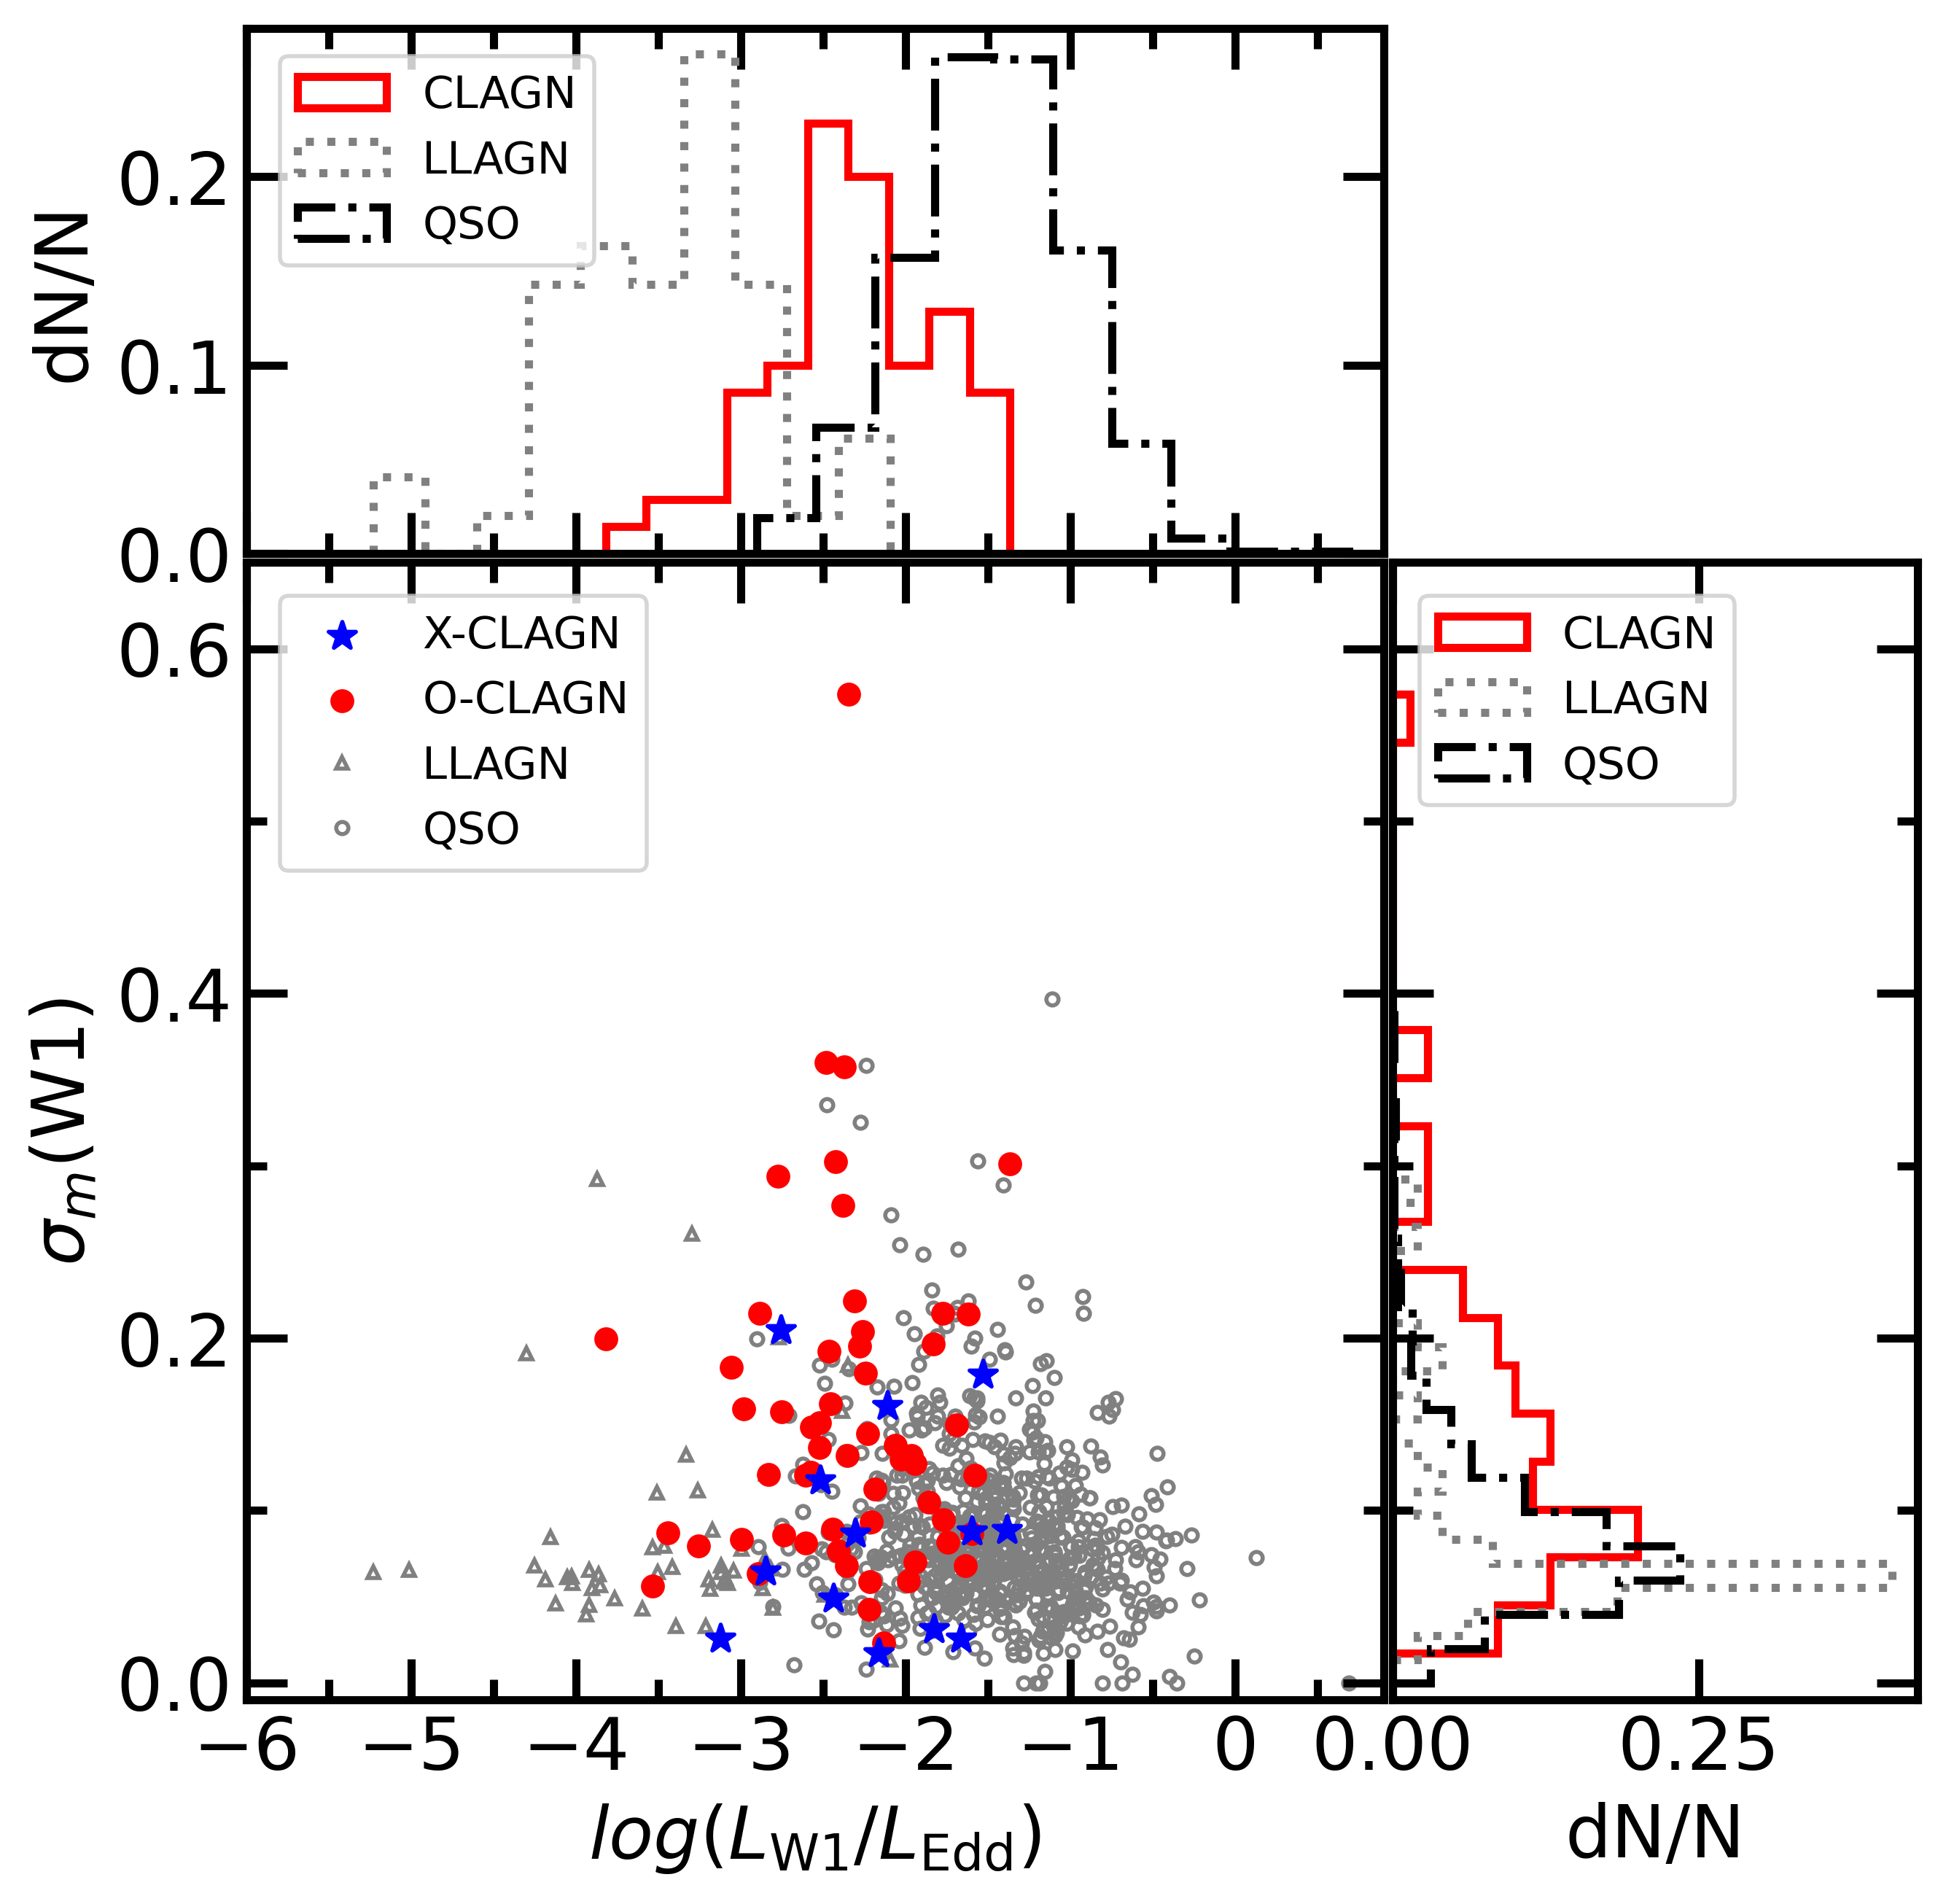
\includegraphics[width=0.5\textwidth]{pic/WISE_var_LW1_Ledd_hist.png}
    \caption{The correlation between the variability of $W1$ band and the mean Eddington-scaled $W1$ band luminosity for LLAGNs \citep{2009MNRAS.399..349G}, CLAGNs, and QSOs \citep{2007ApJ...667..131G} and their distributions. }
    \label{fig:var_ledd_hist}
\end{figure}


\begin{figure}
\centering
	% To include a figure from a file named example.*
	% Allowable file formats are eps or ps if compiling using latex
	% or pdf, png, jpg if compiling using pdflatex
	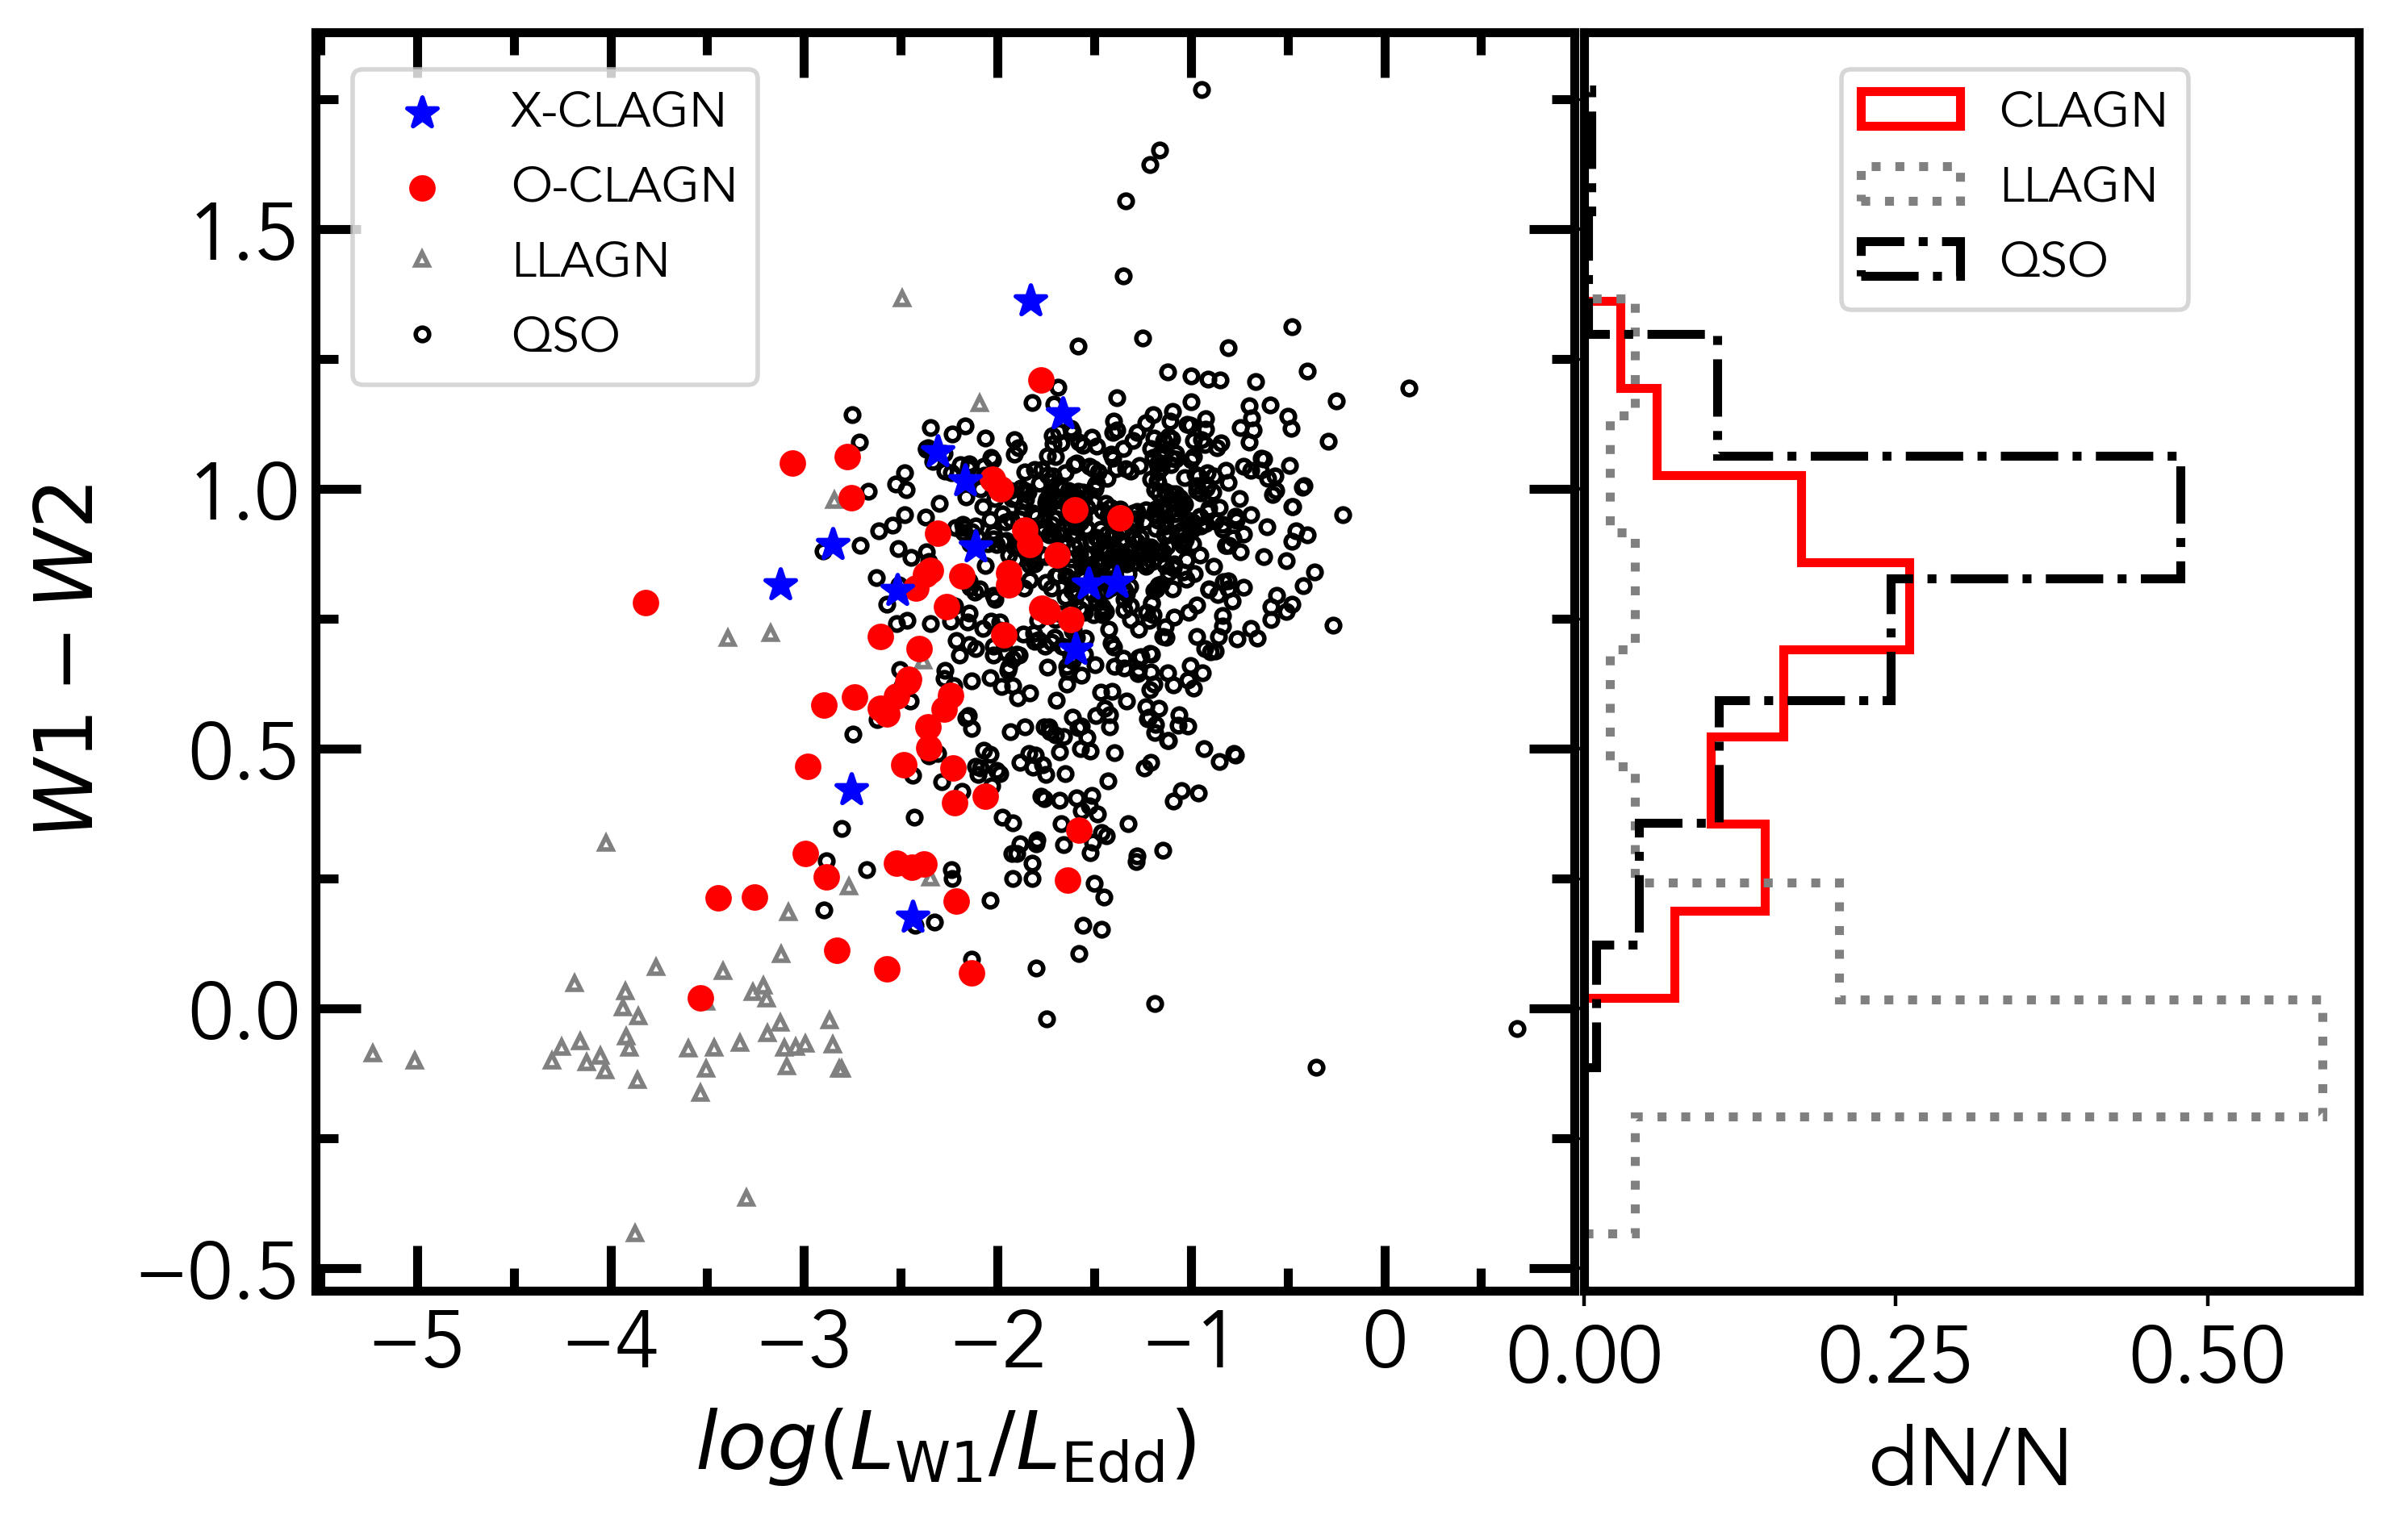
\includegraphics[width=0.5\textwidth]{pic/WISE_W1-W2_LW1_Ledd_hist.png}
    \caption{Distribution of the color for $W1-W2$ and its correlation with the Eddington-scaled $W1$ band luminosity for LLAGNs\citep{2009MNRAS.399..349G}, CLAGNs, and QSOs \citep{2007ApJ...667..131G}. }
    \label{fig:color_ledd}
\end{figure}

\begin{table}
 \caption{Mid-IR variability, color, and Eddington ratio for LLAGNs, CLAGNs, and QSOs.
}
 \label{table_MIR_var_cor_lum}
 \begin{center}
 \begin{tabular}{lccccc}
 \hline\hline
Sample             & LLAGN &   \multicolumn{3}{c}{CLAGN}        & QSO  \\ 
                   &        &   O & X   & All-CLAGN         &       \\ \hline
$<\sigma_{m \mathrm{W1}}>$    &  0.08      & 0.15    &  0.09  &   0.14   &   0.09  \\ 
$<\sigma_{m \mathrm{W2}}>$    &  0.07      &   0.17 &  0.08   &    0.15  &   0.08    \\ 
$<W1-W2>$          &   0.08      &  0.61   & 0.84      &    0.65    &   0.83   \\ 
$<\mathrm{log} L_\mathrm{W1}/L_\mathrm{bol}>$ & -3.46  &  -2.36  &  -2.18   &  -2.33   &  -1.48\\ 
$<\mathrm{log} L_\mathrm{W2}/L_\mathrm{bol}>$ & -3.81  &   -2.5   &  -2.23   &  -2.45   &   -1.53  \\  
\hline\hline
\end{tabular}
\end{center}
\end{table}


\section{Dust reverberation mapping in CLAGNs}\label{sec:tau-L}
Dust reverberation mapping provides a method to explore the properties of AGN torus, where the changes of the disk emission will lead to the variation of infrared emission from the torus but with a time lag due to the signal travel. The continued observations of {\it WISE}, combined with several ground-based optical transient surveys (e.g., All-sky Automated Survey for Supernovae, ASAS-SN) and space-telescope observations (e.g., \swift\,), offer a good opportunity to explore the possible dust structures in these CLAGNs. We adopt the data of $V$ band from the ASAS-SN \citep[][]{2014ApJ...788...48S,2017PASP..129j4502K,2019MNRAS.485..961J}, \uvot\, and mid-IR data from the {\it WISE} to estimate the mid-IR time lag ($\tau$) for CLAGNs. We select 22 bright CLAGNs (e.g., $<W1>$ less than 11 mag) with strong mid-IR variation ($\Delta W1>0.3$ mag), which have good $V$ band and mid-IR band monitorings. For NGC 1566, we adopt the photometric $V$ band data of NGC 1566 from the ASAS-SN and \uvot\,, and the re-binned $W1$/$W2$ band data from the {\it WISE} in each visit to estimate the time lag. We use the tool \textit{uvotmaghist} to do the aperture photometry for V-band data of \uvot\,. The source aperture radius is 3$\arcsec$ and the background is a blank region with a much larger radius. We find that the flux of NGC 1566 in ASAS-SN is systematically higher than that of \uvot\,, which is probably contaminated by the host galaxy due to the poor angular resolution \citep[see ][]{2017PASP..129j4502K}. We then subtract the average offset of V-band data from ASAS-SN data, which is determined from the quasi-simultaneous (within 1 day of the interval) observations of ASAS-SN and \uvot\,. For other sources, we only use the $V$ band data from ASAS-SN and the re-binned $W1$/$W2$ data in each visit with good observational overlaps to estimate the time lags. The $V$ band data are binned in 30 days for some sources with complex short-term variability.

We use the interpolation cross-correlation function \citep[ICCF;][]{1998PASP..110..660P,2018ascl.soft05032S} in a range of 0--400 days (corresponding to $\sim 70000 R_g$ for $M_\mathrm{BH}=10^8 M_{\odot}$) for the first attempt to estimate $\tau$ and then further limited the range according to the posterior of $\tau$. The interpolation time steps of 5 days are applied to the $V$ and the $W1$/$W2$ band light curves. The flux randomization and random subset selection methods are employed with 50000 realizations in the Monte Carlo simulation to estimate the centroid time lags and the uncertainties\footnote{The code \texttt{pyCCF} is available in \url{http://ascl.net/code/v/1868}}. We also use {\sc javelin} algorithm to further test the results of the ICCF method, where {\sc javelin} algorithm fits the light curves using a damped random walk (DRW) model with amplitude and time scale of the variability. A top-hat transfer function (TF) is convolved with the driving light curve and the best-fit model parameters such as time lag $\tau$ are found through the Markov Chain Monte Carlo method. We restrict the lag and width in the range of 0--400 days for the first attempt. Finally,  we get time lag measurements of 15 sources with maximum cross-correlation coefficient $r>0.6$, which are shown in Figure 3 and \autoref{lag_analysis}. In most cases, two methods give the roughly consistent results. Later on, we adopt the time lags from the {\sc javelin} method as primary results in the following analysis, where the time lags are listed in \autoref{table_lag}. 

\begin{figure}[b]\label{fig:lag_NGC1566}
\begin{tikzpicture}
    \matrix[matrix of nodes]{
    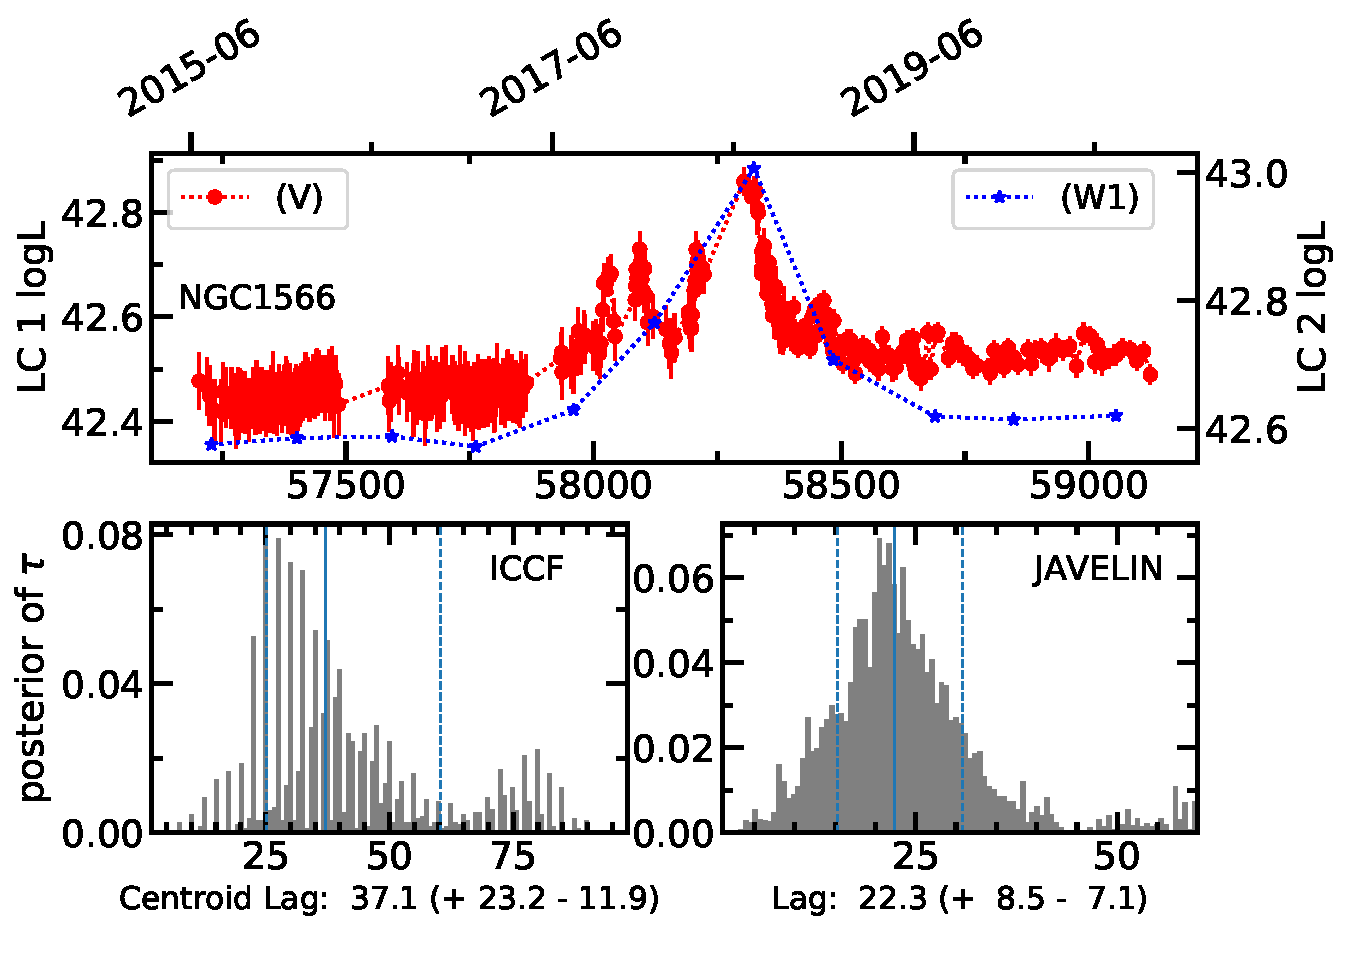
\includegraphics[width=0.45\textwidth]{pic/lag_pic/NGC1566_lag.pdf} & \hspace{1em} & 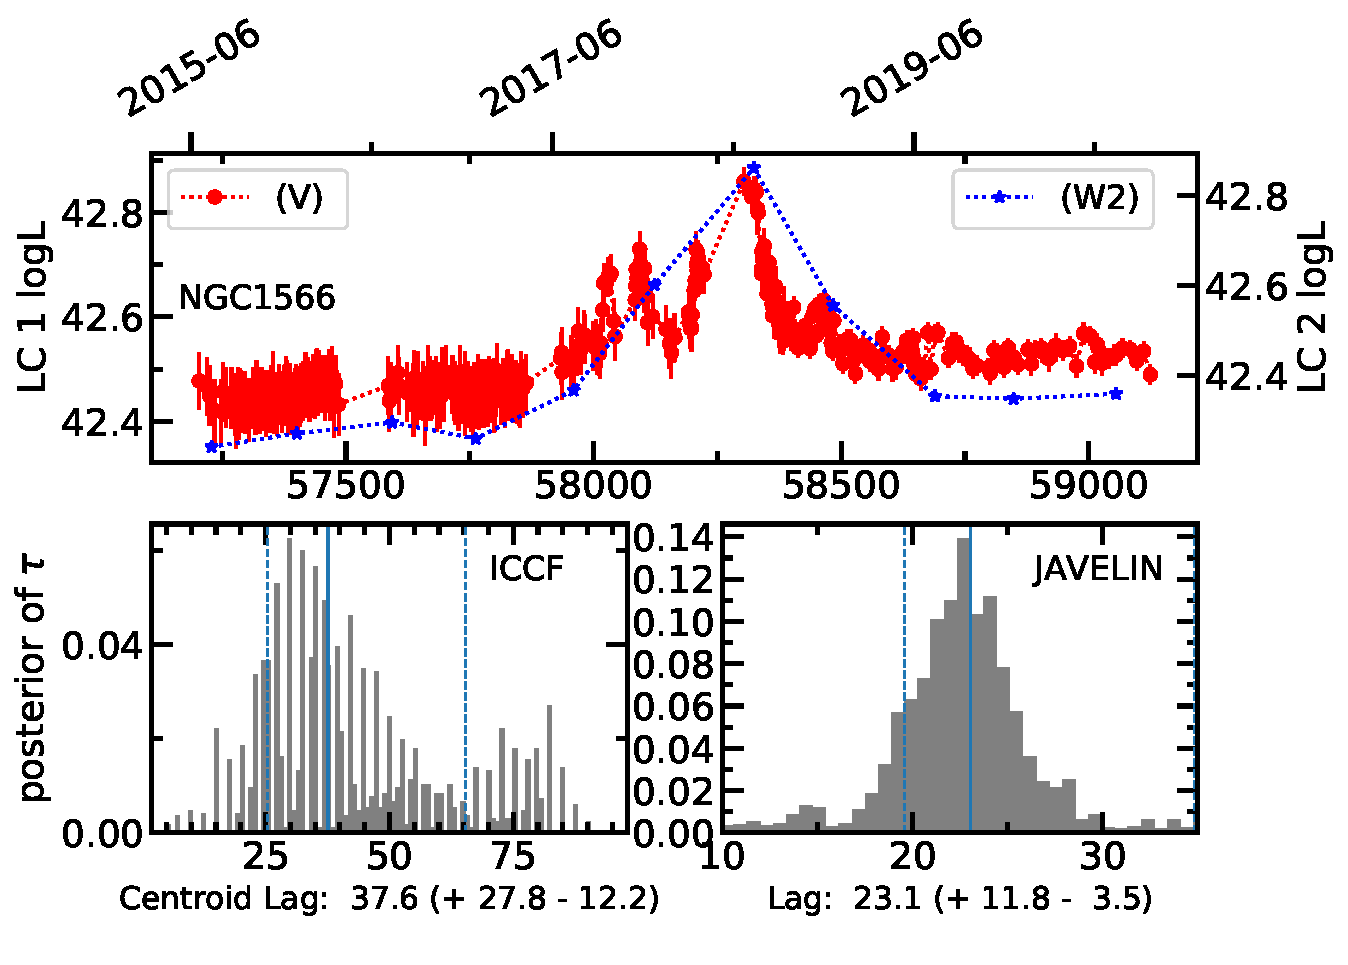
\includegraphics[width=0.45\textwidth]{pic/lag_pic/NGC1566_lag_w2.pdf} \\
    };
\end{tikzpicture}
\caption{Dust reverberation mapping analysis result for NGC 1566 as an example, and other sources are presented in Appendix. Left panel shows the light curves and the posterior of time lag between $V$ and $W1$ band. Right panel shows the light curves and the posterior of time lag between $V$ and $W2$ band.}
\end{figure}

\begin{table}
\renewcommand{\arraystretch}{1.5}
 \caption{Mid-IR time lag results of CLAGNs.
}
 \label{table_lag}
 \begin{center}
 \begin{tabular}{lccccccc}
 \hline\hline
Name & log($L_\mathrm{bol}$) & \multicolumn{2}{c}{$\tau_\mathrm{W1}$} & \multicolumn{2}{c}{$\tau_\mathrm{W2}$} &Type \\ 
      &                      &   ICCF     &  {\sc javelin}   &    ICCF & {\sc javelin} &   \\ \hline 
3C 390.3 & 45.79 & $180.5_{-16.6}^{+18.9}$ & $186.5_{-9.5}^{+11.3}$ & $184.8_{-21.3}^{+25.0}$ & $200.1_{-10.6}^{+26.4}$ & O \\
HE 1136-2304 & 44.31 & $127.6_{-43.9}^{+68.3}$ & $178.7_{-47.6}^{+54.9}$ & $177.0_{-62.6}^{+70.6}$ & $196.8_{-28.9}^{+50.8}$ & O \\
Mrk 530 & 44.90 & $212.2_{-39.7}^{+15.2}$ & $215.2_{-6.5}^{+6.1}$ & $215.0_{-20.3}^{+12.9}$ & $216.8_{-6.5}^{+11.4}$ & O \\
Mrk 590 & 44.13 & $57.9_{-20.0}^{+17.8}$ & $97.0_{-29.2}^{+30.6}$ & $56.6_{-21.3}^{+13.8}$ & $115.0_{-36.5}^{+30.1}$ & O \\
Mrk 6 & 44.59 & $141.6_{-11.0}^{+31.7}$ & $170.3_{-15.4}^{+13.5}$ & $180.4_{-15.1}^{+16.6}$ & $222.8_{-34.8}^{+9.1}$ & O \\
Mrk 609 & 44.43 & $173.0_{-37.9}^{+43.6}$ & $239.9_{-19.0}^{+33.0}$ & $187.0_{-60.7}^{+49.5}$ & $262.3_{-18.8}^{+19.5}$ & O \\
Mrk 926 & 45.66 & $213.8_{-31.0}^{+25.3}$ & $242.1_{-9.8}^{+11.7}$ & $252.5_{-38.3}^{+27.5}$ & $273.1_{-13.3}^{+14.2}$ & O \\
NGC 1566 & 42.94 & $37.1_{-11.9}^{+23.2}$ & $22.3_{-7.1}^{+8.5}$ & $37.6_{-12.2}^{+27.8}$ & $23.1_{-3.5}^{+11.8}$ & O \\
NGC 2617 & 43.77 & $93.8_{-17.6}^{+17.0}$ & $69.8_{-12.6}^{+11.9}$ & $93.5_{-17.0}^{+19.1}$ & $73.9_{-16.0}^{+9.7}$ & O \\
NGC 3516 & 44.19 & $91.1_{-31.4}^{+64.0}$ & $88.5_{-34.1}^{+48.5}$ & $100.7_{-28.5}^{+54.4}$ & $119.8_{-37.5}^{+43.3}$ & O \\
NGC 4051 & 42.61 & $22.3_{-10.0}^{+10.4}$ & $26.2_{-11.4}^{+17.0}$ & $24.8_{-12.2}^{+10.2}$ & $29.0_{-12.3}^{+20.9}$ & X \\
NGC 4151 & 44.08 & $74.4_{-19.5}^{+40.8}$ & $77.6_{-12.9}^{+26.1}$ & $99.3_{-32.6}^{+40.7}$ & $89.4_{-12.2}^{+17.0}$ & O \\
NGC 5548 & 44.66 & $162.7_{-31.7}^{+37.2}$ & $132.0_{-4.8}^{+5.7}$ & $207.3_{-29.0}^{+25.7}$ & $236.3_{-5.7}^{+4.7}$ & O \\
NGC 7469 & 44.53 & $131.2_{-22.4}^{+37.9}$ & $145.9_{-11.9}^{+8.5}$ & $159.7_{-29.5}^{+39.4}$ & $152.4_{-11.2}^{+17.5}$ & X \\
PG 1535+547 & 45.15 & $155.0_{-25.6}^{+22.0}$ & $169.3_{-4.0}^{+11.7}$ & $160.9_{-35.4}^{+19.5}$ & $176.4_{-5.3}^{+6.4}$ & X \\
\hline\hline
\end{tabular}
\end{center}
Note. The table lists source name, bolometric luminosity, time lag between $V$ band and $W1$/$W2$ band from the ICCF and {\sc javelin} method , CLAGN type (``O'' for optical CLAGN and ``X'' for X-ray CLAGN). 
\end{table}


To explore the possible correlation between time lag ($\tau$) and bolometric luminosity ($L_\mathrm{bol}$), we estimate the bolometric luminosities of CLAGNs from the X-ray luminosity through a bolometric correction of $L_{\mathrm{bol}}=8 \times L_{\mathrm{14-195 keV }}$ \citep[e.g.,][]{2009MNRAS.392.1124V}, where the X-ray data are obtained from the 105-Month Swift-BAT All-sky Hard X-Ray Survey reported in \citet{2018ApJS..235....4O}. PG 1535+547 is not included in the above \bat\, survey and we adopt $L_{\mathrm{\rm bol}}\sim 1.4\times \, 10^{45} erg\, s^{-1}$, which is estimated from [O~{\small III}] line width by \citet{2006ApJ...653..137Z}. The correlation between $\tau_{\rm{W1}}$/$\tau_{\rm{W2}}$ and $L_\mathrm{bol}$ for CLAGNs is shown in \autoref{fig:tau_L}.

It can be found that the brighter CLAGNs have longer time lags (Spearman's rank correlation coefficient $r=0.82$ with a probability of $p=1.7\times10^{-4}$ for $\tau_{\rm{W1}}$-$L_\mathrm{bol}$ and $r=0.81$ with a probability of $p=2.5\times10^{-4}$ for $\tau_{\rm{W2}}$-$L_\mathrm{bol}$). We use UltraNest\footnote{\url{https://johannesbuchner.github.io/UltraNest/}} package, which implements nested sampling to constrain the model parameters \citep{2021JOSS....6.3001B}, to fit the linear log$\tau$-log($L_{\mathrm{bol}}$) correlation for the 15 CLAGNs using the following equation: 
\begin{equation}
\mathrm{log}(\tau/\mathrm{day})=a\times\mathrm{log}(L_{\mathrm{bol}}/10^{11} L_{\odot})+b.
\end{equation}

We get \begin{equation}
\mathrm{log}(\tau_{\rm{W1}}/\mathrm{day})= 0.28^{+0.07}_{-0.06}\times \mathrm{log}(L_{\mathrm{bol}}/10^{11} L_{\odot})+ 2.12^{+0.05}_{-0.05}
\end{equation} for the $W1$ band, and 
\begin{equation}
\mathrm{log}(\tau_{\rm{W2}}/\mathrm{day})= 0.28^{+0.06}_{-0.06}\times \mathrm{log}(L_{\mathrm{bol}}/10^{11} L_{\odot})+ 2.20^{+0.04}_{-0.05}
\end{equation}for the $W2$ band. The CLAGNs still follow a consistent $\tau$-$L_{\mathrm{bol}}$ correlation with that found for the 87 luminous Palomar--Green quasars \citep[usually with $L_{\mathrm{bol}} \ge 10^{11}L_{\odot}$, see ][]{2019ApJ...886...33L} within the scatter, and the best fitting results are listed in \autoref{table_tau_L_fit}.




\begin{figure}[h!]
\centering
	% To include a figure from a file named example.*
	% Allowable file formats are eps or ps if compiling using latex
	% or pdf, png, jpg if compiling using pdflatex
	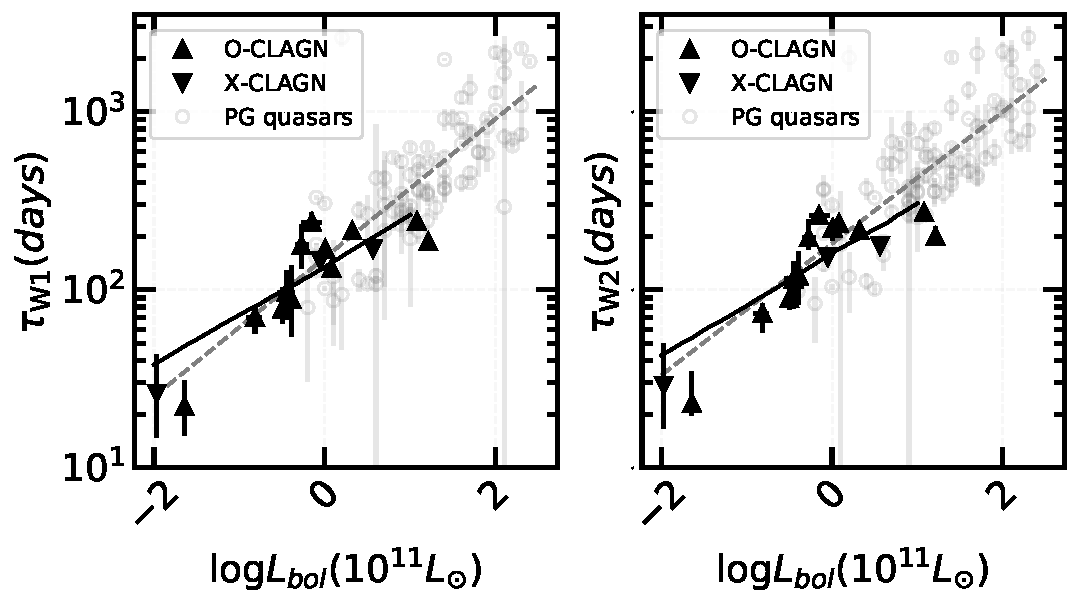
\includegraphics[width=0.6\textwidth]{pic/tau_L_correlation_clagn_J_w1_w2.pdf}
    \caption{The correlation between the time lag $\tau$ and the bolometric $L_{\rm bol}$ for CLAGNs, where $\tau$ is the time lag between $V$ band and $W1$/$W2$ band. The solid line is the best fitting for CLAGNs. Grey circles represent PG quasars \citep{2019ApJ...886...33L} for comparison. The dashed line represents the best fitting for PG quasars in \citet{2019ApJ...886...33L} and the CLAGNs in this work. } 
    \label{fig:tau_L}
\end{figure}

\begin{table}[h!]
\renewcommand{\arraystretch}{1.5}
 \caption{The best fitting results of $\tau$-$L_{\mathrm{bol}}$ correlation for CLAGNs and QSOs through UltraNest package.
}
 \label{table_tau_L_fit}
 \begin{center}
 \begin{tabular}{lcccccc}
 \hline\hline
Sample    & \multicolumn{3}{c}{$W1$} &   \multicolumn{3}{c}{$W2$}      \\ %\hline
           &    $a$    & $b$   &    scatter   &  $a$            &     $b$    & scatter        \\ \hline
CLAGNs      &    $0.28^{+0.07}_{-0.06}$ & $2.12^{+0.05}_{-0.05}$ & $0.14^{+0.04}_{-0.03}$  & $0.28^{+0.06}_{-0.06}$  &  $2.20^{+0.04}_{-0.05}$     &  $0.15^{+0.05}_{-0.03}$  \\ 
PG quasars    &    $0.39^{+0.04}_{-0.04}$ & $2.19^{+0.05}_{-0.06}$  &   $0.23^{+0.02}_{-0.02}$   & $0.36^{+0.04}_{-0.04}$  & $2.29^{+0.06}_{-0.05}$    & $0.22^{+0.02}_{-0.02}$  \\
CLAGNs \& PG quasars &   $0.39^{+0.03}_{-0.03}$ & $2.18^{+0.03}_{-0.03}$ & $0.22^{+0.02}_{-0.01}$ & $0.37^{+0.03}_{-0.03}$   & $2.26^{+0.04}_{-0.04}$        &$0.21^{+0.02}_{-0.02}$   \\ 

\hline\hline
\end{tabular}
\end{center}
Note. The slope (a), intercept (b) and scatter of the best fitting for $\tau$-$L_{\mathrm{bol}}$ correlation. The data of PG quasars are adopted from \citet{2019ApJ...886...33L}.
\end{table}


\section{Conclusion and Discussion} \label{sec:dis}
We perform an analysis on the {\it WISE} mid-IR data for a sample of both X-ray and optical CLAGNs to explore the possible physical mechanism behind them. We find that the Eddington scaled mid-IR luminosity of CLAGNs is lower than that of QSOs but higher than that of LLAGNs. A large fraction of CLAGNs show strong mid-IR variabilities, where the average variability $<\sigma_{m}>$ is almost two times larger than that of both LLAGNs and QSOs. The color of $W1-W2$ also shows a wider distribution in CLAGNs, where brighter and fainter CLAGNs are similar to QSOs and LLAGNs, respectively. The above results support that the CLAGNs possibly stay in a transitional stage, where the moderate Eddington ratio and the strong variability may be triggered by the fast transition of accretion mode at a critical accretion rate. Based on the mid-IR and optical variability, we estimate the dust echo time lags of 15 CLAGNs, which roughly follow the correlation of $\tau-L_\mathrm{bol}$ as found in the QSOs \citep{2019ApJ...886...33L}. 



%A $\tau-L_\mathrm{bol}$ correlation consistent with QSOs \citep{2019ApJ...886...33L} supports the same dust echo process existing in CLAGNs and luminous AGNs. 

%


\subsection{Transitional stage of CLAGNs}
The study of the intrinsic physics of CLAGNs will help us to understand the nature of accretion flow and the evolution of galaxies. Since the mid-IR emission is mainly produced by the hot dust heated by the UV radiation of the accretion disk, the mid-IR properties of CLAGNs can shed light on their central engines. The physical mechanism for CLAGNs is still unclear, especially for X-ray CLAGNs. We find that the most of the CLAGNs show strong variation in the mid-IR band (e.g., more than 70\% sources have maximum variation magnitude $\Delta W1>0.3$). The variation suggests that most of the optical and X-ray CLAGNs cannot be simply explained by the motion of absorbing clouds moving in/out of our line of sight, where the ``changing-look'' should be correlated with the variation of the accretion disk (e.g., change of disk structure, disk wind, etc). The Eddington ratio of mid-IR luminosity for CLAGNs just stays between QSOs and LLAGNs, where the standard accretion disk and ADAF are widely believed in QSOs and LLAGNs, respectively. The average ratio of $L_\mathrm{W1}/L_\mathrm{Edd}$ for CLAGNs is $\sim $0.5\%, which roughly corresponds to $L_\mathrm{bol}/L_\mathrm{Edd}\sim$ several percent by assuming a bolometric correction factor of $\sim 10$ \citep[e.g.,][]{2012MNRAS.426.2677R}. The multi-epoch observations of several CLAGNs also show that they cross a critical bolometric Eddington ratio of $L_\mathrm{bol}/L_\mathrm{Edd}\sim$1\% during their dramatic variations \citep[e.g.,][]{2019ApJ...883...76R,2021MNRAS.508..144G,2021MNRAS.506.4188L,2021MNRAS.507..687J}, which is similar to the state transition in black hole X-ray binaries \citep[e.g.,][]{2008ApJ...682..212W}. We find that the CLAGNs show stronger mid-IR variation compared to LLAGNs and QSOs (see \autoref{fig:var_ledd_hist}), which may be triggered by the quick disk transition between SSD and ADAF at a critical accretion rate of $\sim$1\% Eddington ratio. The CLAGNs will show galaxy-like mid-IR color (e.g., $W1-W2\leq0.5$) when the sources enter into the faint state, while they will show AGN-like mid-IR color (e.g., $W1-W2\geq0.5$) when the sources enter into the bright state and vice versa \citep[e.g.,][]{2012ApJ...753...30S,2013AJ....145...55Y,2020ApJ...889...46S}. Therefore, the color distribution of CLAGNs also supports the possible disk transition in CLAGNs. 

As the accretion rate decreases below the critical value, the inner cold disk might transit into ADAF and the intrinsic luminosities will drop, which will reduce the ionizing photons for exciting the broad emission lines. The AGNs will change their optical type from type 1 to type 1.5-1.8 or even type 2 as seen in the optical CLAGNs. The sources will go back to type 1 state when the SSD is reformed as the accretion rate increases. 

In this work, we find around half of X-ray CLAGNs show strong mid-IR variability and they also have a moderate distribution of mid-IR Eddington ratios, where the mid-IR properties of X-ray CLAGNs are not much different from the optical ones. We suggest that the X-ray CLAGNs may be also triggered by the possible change of accretion flow. The formation of disk wind and its opening angle are closely correlated to the underlying SSD \citep[e.g.,][]{2017PASA...34...42Y,2020MNRAS.492.5540M}. Therefore, we suggest that X-ray CLAGNs may appear in CLAGNs with a moderate inclination angle (e.g., $40^{\rm o}$-$60^{\rm o}$), where the line of sight will cross the disk winds. The X-ray spectral evolution in a X-ray CLAGN of NGC 1365 does support this scenario \citep[e.g.,][]{2014MNRAS.440.3503C,2021RAA....21..199L}.


\subsection{Dust echo in CLAGNs}
Mid-IR emission at $W1$ and $W2$ band mainly comes from the hot dust heated by central engine of AGNs. The dust reverberation mapping method can be applied when the source has strong optical and mid-IR variability. We explore the dust echo time lag $\tau$ for 15 CLAGNs based on mid-IR and optical multi-epoch observations, which include 12 optical CLAGNs and 3 X-ray CLAGNs. Several CLAGNs are famous nearby Seyferts, where the infrared reverberation mappings have been explored in the previous works. The mid-IR time lags ($\tau_{\mathrm{W1}} \sim 180\pm 1.4$ days and $\tau_{\mathrm{W2}}\sim 207.7\pm 0.2$ days) for PG 1535+547 reported in \citet{2019ApJ...886...33L} are roughly consistent with our results (see \autoref{table_lag}). The time lags between $K$ band (2.19 $\mu$m) and $V$ band of 6 CLAGNs (Mrk 590, NGC 3516, NGC 4051, NGC 4151, NGC 5548, and NGC 7469) in a sample of 17 Seyfert 1 AGNs have been reported \citep[see][]{2014ApJ...788..159K,2019ApJ...886...33L}. Adopting the time-lag ratio $\tau_{\mathrm{K}}$: $\tau_{\mathrm{W1}}$=$0.6$: $1$ \citep[see][]{2019ApJ...886...33L}, the derived time lags for the 6 CLAGNs from \citet[]{2014ApJ...788..159K} are roughly consistent with our results. The time-lag ratio $\tau_{\mathrm{W1}}$: $\tau_{\mathrm{W2}}$=$1$: $1.2$ for the 15 CLAGNs is also consistent with that of the luminous QSOs \citep[see][]{2019ApJ...886...33L}. The positive correlation between mid-IR time lag and bolometric luminosity ($\tau$-$L$) for AGNs has been widely investigated \citep[e.g.,][]{2014ApJ...788..159K,2019ApJ...886...33L,2019ApJ...886..150M,2020MNRAS.495.2921N,2020AJ....159..259S,2021MNRAS.501.3905M}. In CLAGNs, there is also a tight $\tau$-$L$ correlation, which is roughly consistent with that of the luminous QSOs \citep{2019ApJ...886...33L} within the errorbar (see \autoref{fig:tau_L}). The time lag of mid-IR band suggests the similar circumnuclear dust structure existing both in CLAGNs and QSOs. The $\tau$-$L$ correlation for CLAGNs is slightly shallower than expected $\tau \propto L^{0.5}$ assuming the similar dust sublimation temperature \citep{2013peag.book.....N} and a face-on viewing angle \citep{2019ApJ...886...33L}. The physical reason for this shallower slope is unclear, which might be influenced by the structure of the torus or the inclination angle.  



\begin{acknowledgments}
BL and QW were supported in part by the Natural Science Foundation of China (grant U1931203) and the science research grants from the China Manned Space Project with NO. CMS-CSST-2021-A06; ZY was supported in part by the Natural Science Foundation of China (grants 11773055 and U1938114), the Youth Innovation Promotion Association of CAS (id 2020265); and WY would like to acknowledge the support in part by the National Program on Key Research and Development Project (grant 2016YFA0400804) and the National Natural Science Foundation of China (grants 11333005 and U1838203).
%\vspace{5mm}
This research has made use of WISE and NEOWISE data products from the NASA/IPAC Infrared Science Archive, which is a joint project of the University of California, Los Angeles, and the Jet Propulsion Laboratory/California Institute of Technology, funded by the National Aeronautics and Space Administration. 

%This research has made use of the NASA/IPAC Extragalactic Database (NED) which is operated by the Jet Propulsion Laboratory, Caltech, under contract with the National Aeronautics and Space Administration.
%This research has made use of MAXI data provided by RIKEN, JAXA and the MAXI team.

%Chinese Academy of Sciences
\end{acknowledgments}

%% To help institutions obtain information on the effectiveness of their 
%% telescopes the AAS Journals has created a group of keywords for telescope 
%% facilities.
%
%% Following the acknowledgments section, use the following syntax and the
%% \facility{} or \facilities{} macros to list the keywords of facilities used 
%% in the research for the paper.  Each keyword is check against the master 
%% list during copy editing.  Individual instruments can be provided in 
%% parentheses, after the keyword, but they are not verified.



\facilities{\textit{WISE}, \uvot\,, ASAS-SN}%
%, \maxi\, }
%CTIO:1.3m,CTIO:1.5m,CXO}

%% Similar to \facility{}, there is the optional \software command to allow 
%% authors a place to specify which programs were used during the creation of 
%% the manuscript. Authors should list each code and include either a
%% citation or url to the code inside ()s when available.

\software{astropy \citep{2013A&A...558A..33A,2018AJ....156..123A},  
         \sc{javelin}\citep{2011ApJ...735...80Z,2013ApJ...765..106Z}, 
         \sc{pyccf}\citep{1998PASP..110..660P,2018ascl.soft05032S},
          %Cloudy \citep{2013RMxAA..49..137F}, 
          %Source Extractor \citep{1996A&AS..117..393B}
          }

%% Appendix material should be preceded with a single \appendix command.
%% There should be a \section command for each appendix. Mark appendix
%% subsections with the same markup you use in the main body of the paper.

%% Each Appendix (indicated with \section) will be lettered A, B, C, etc.
%% The equation counter will reset when it encounters the \appendix
%% command and will number appendix equations (A1), (A2), etc. The
%% Figure and Table counter will not reset.


%% For this sample we use BibTeX plus aasjournals.bst to generate the
%% the bibliography. The sample631.bib file was populated from ADS. To
%% get the citations to show in the compiled file do the following:
%%
%% pdflatex sample631.tex
%% bibtext sample631
%% pdflatex sample631.tex
%% pdflatex sample631.tex


\bibliographystyle{aasjournal}
\bibliography{ref.bib}
%% This command is needed to show the entire author+affiliation list when
%% the collaboration and author truncation commands are used.  It has to
%% go at the end of the manuscript.
%\allauthors

%% Include this line if you are using the \added, \replaced, \deleted
%% commands to see a summary list of all changes at the end of the article.
%\listofchanges

\appendix
\section{time lag analysis}\label{lag_analysis}

\begin{figure}[h!]
\begin{tikzpicture}
    \matrix[matrix of nodes]{
    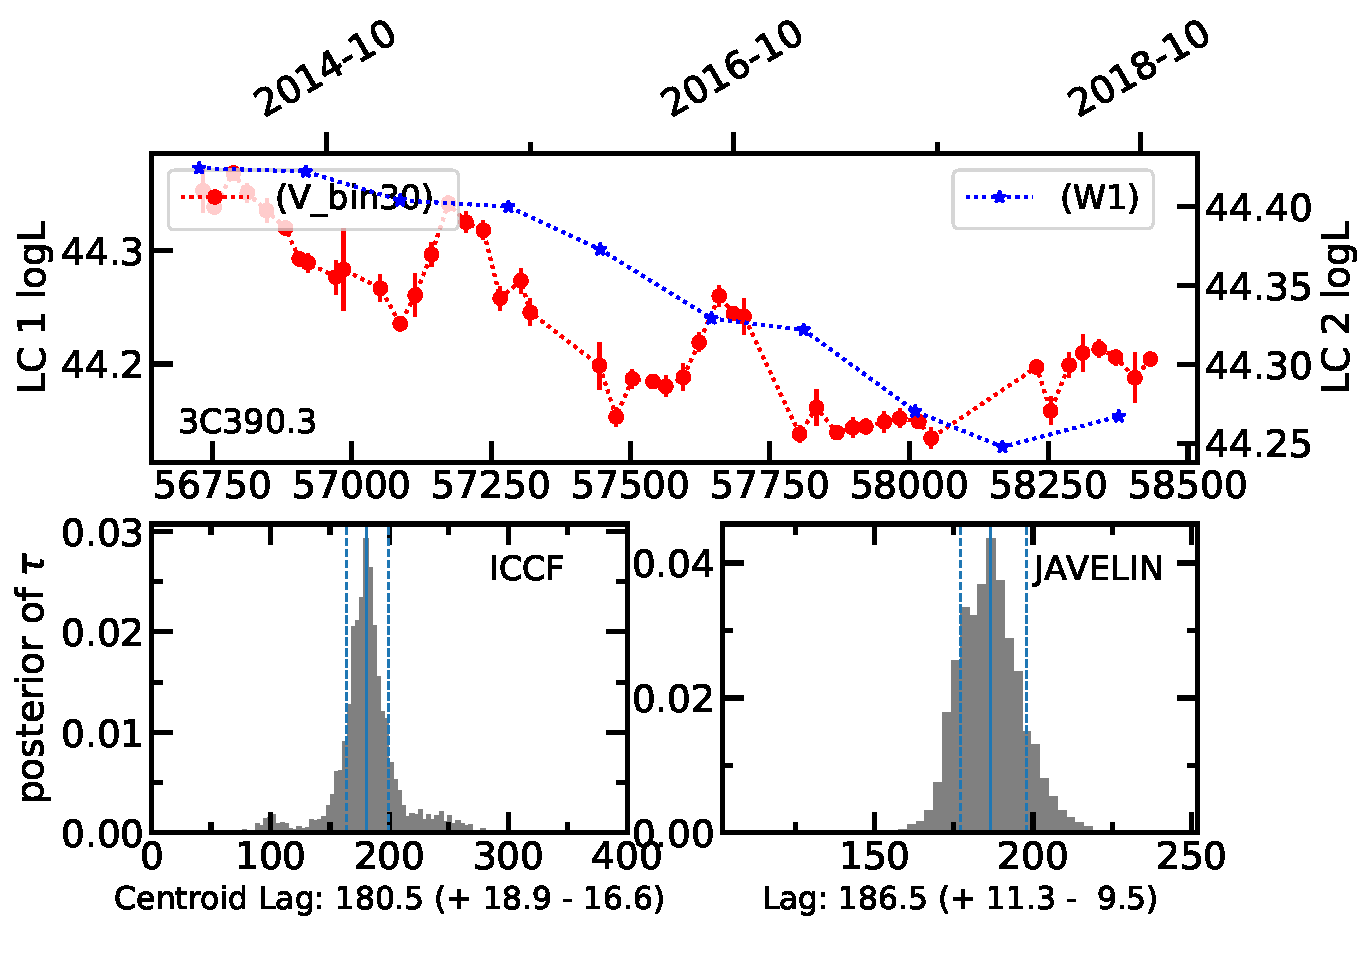
\includegraphics[width=0.45\textwidth]{pic/lag_pic/3C390.3lag1.pdf}& \hspace{1em}  &
    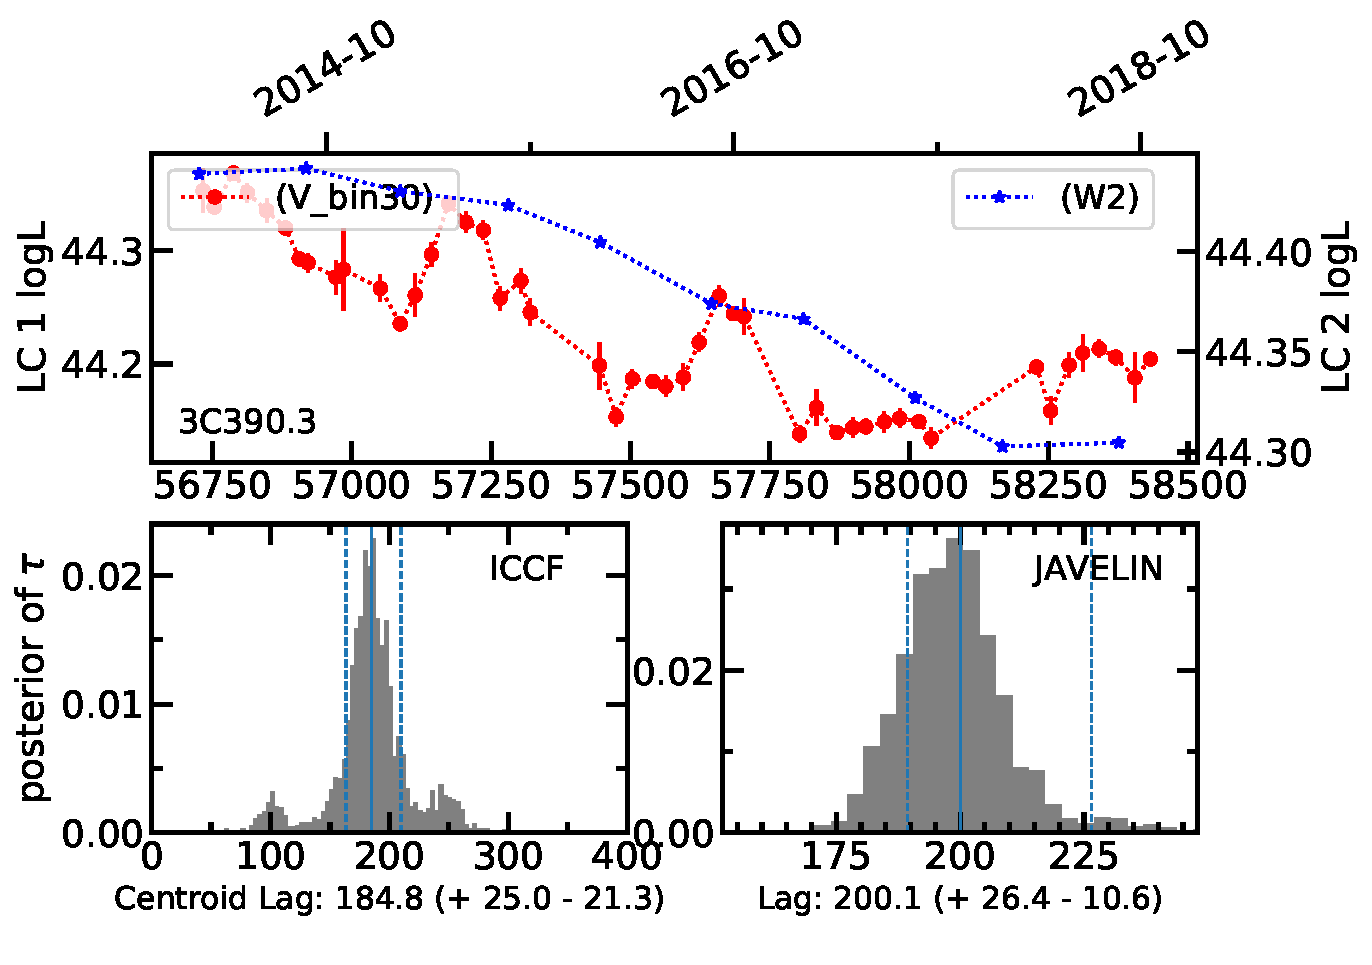
\includegraphics[width=0.45\textwidth]{pic/lag_pic/3C390.3lag1_w2.pdf} \\
    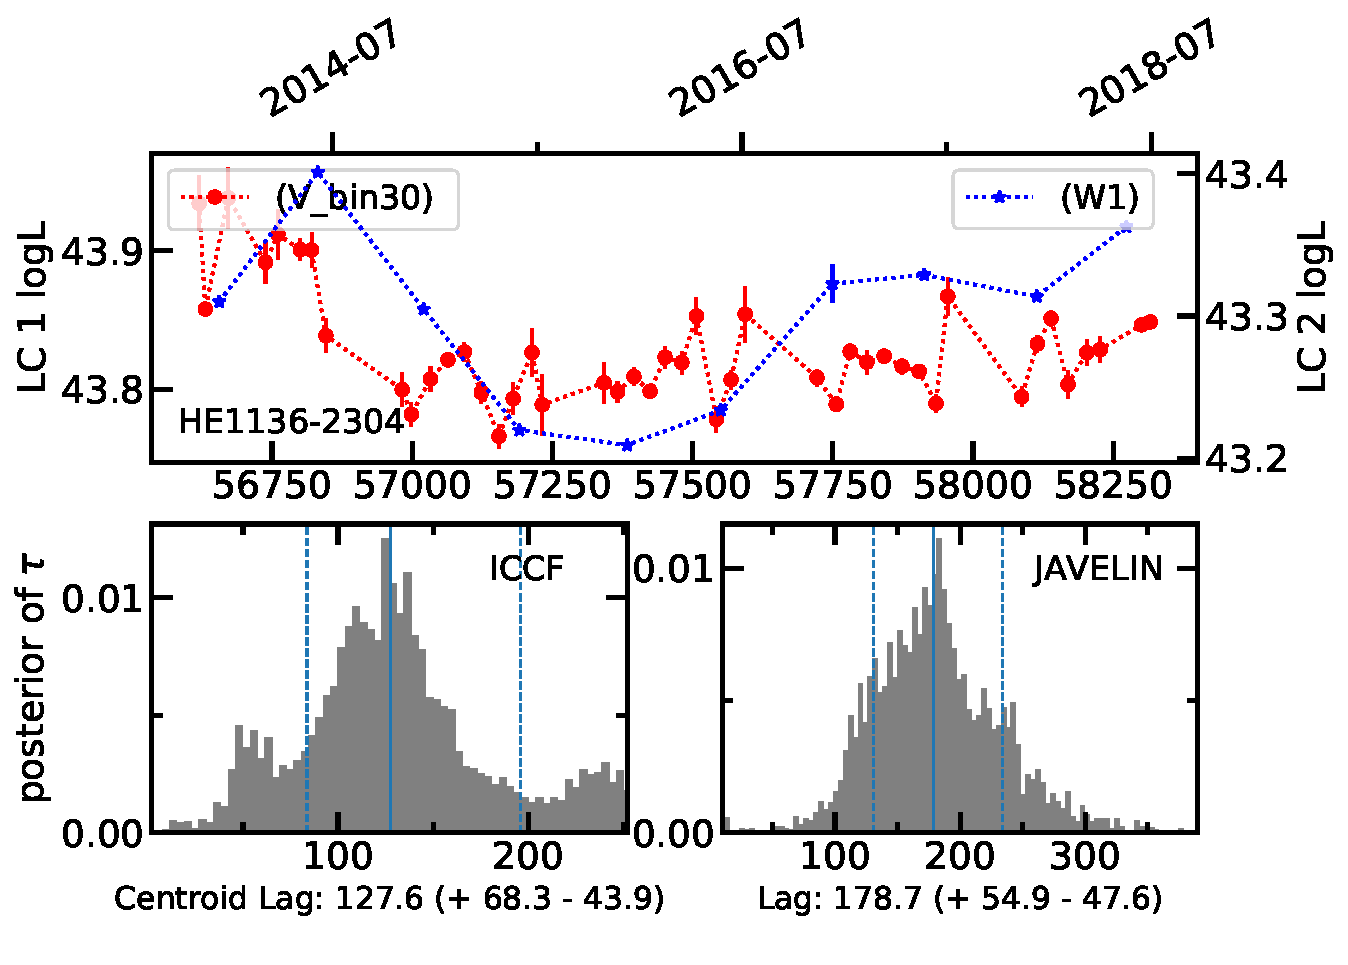
\includegraphics[width=0.45\textwidth]{pic/lag_pic/HE1136-2304lag1.pdf}& \hspace{1em}  &
    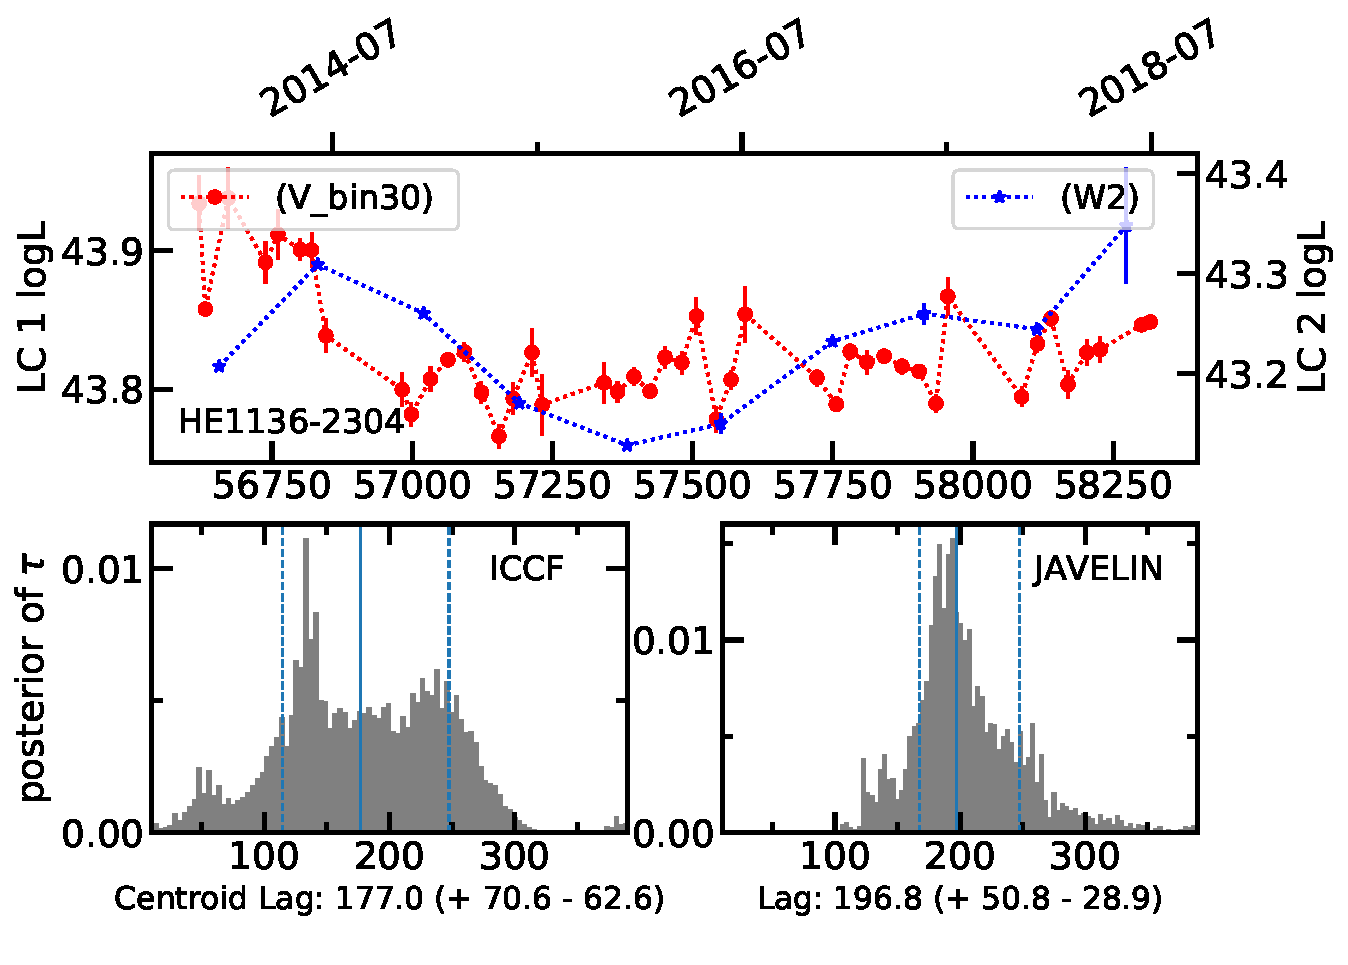
\includegraphics[width=0.45\textwidth]{pic/lag_pic/HE1136-2304lag1_w2.pdf} \\
    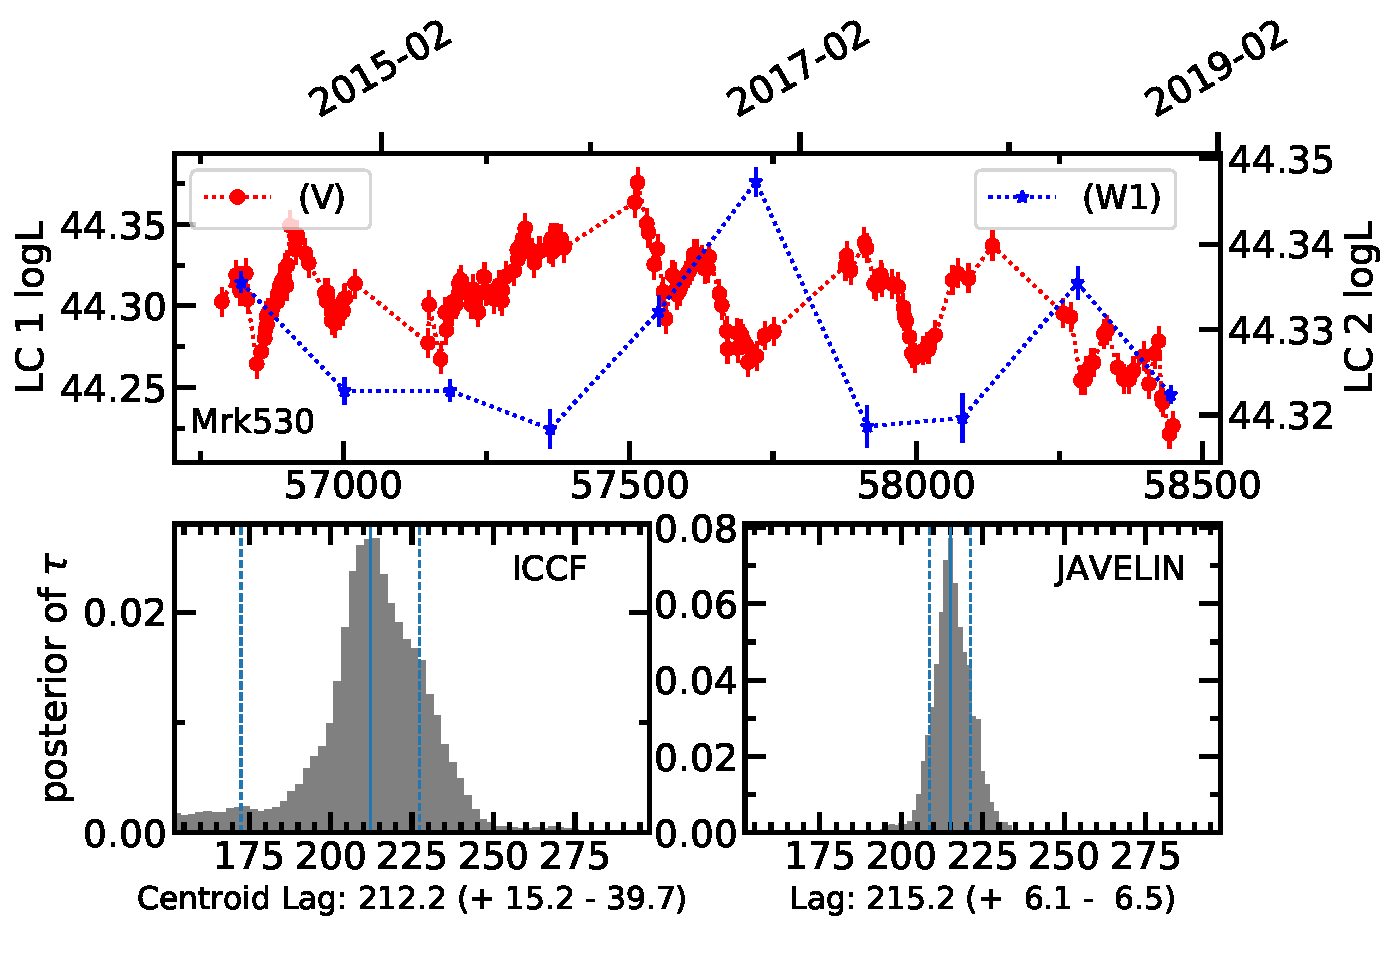
\includegraphics[width=0.45\textwidth]{pic/lag_pic/Mrk530_lag.pdf}& \hspace{1em}  &
    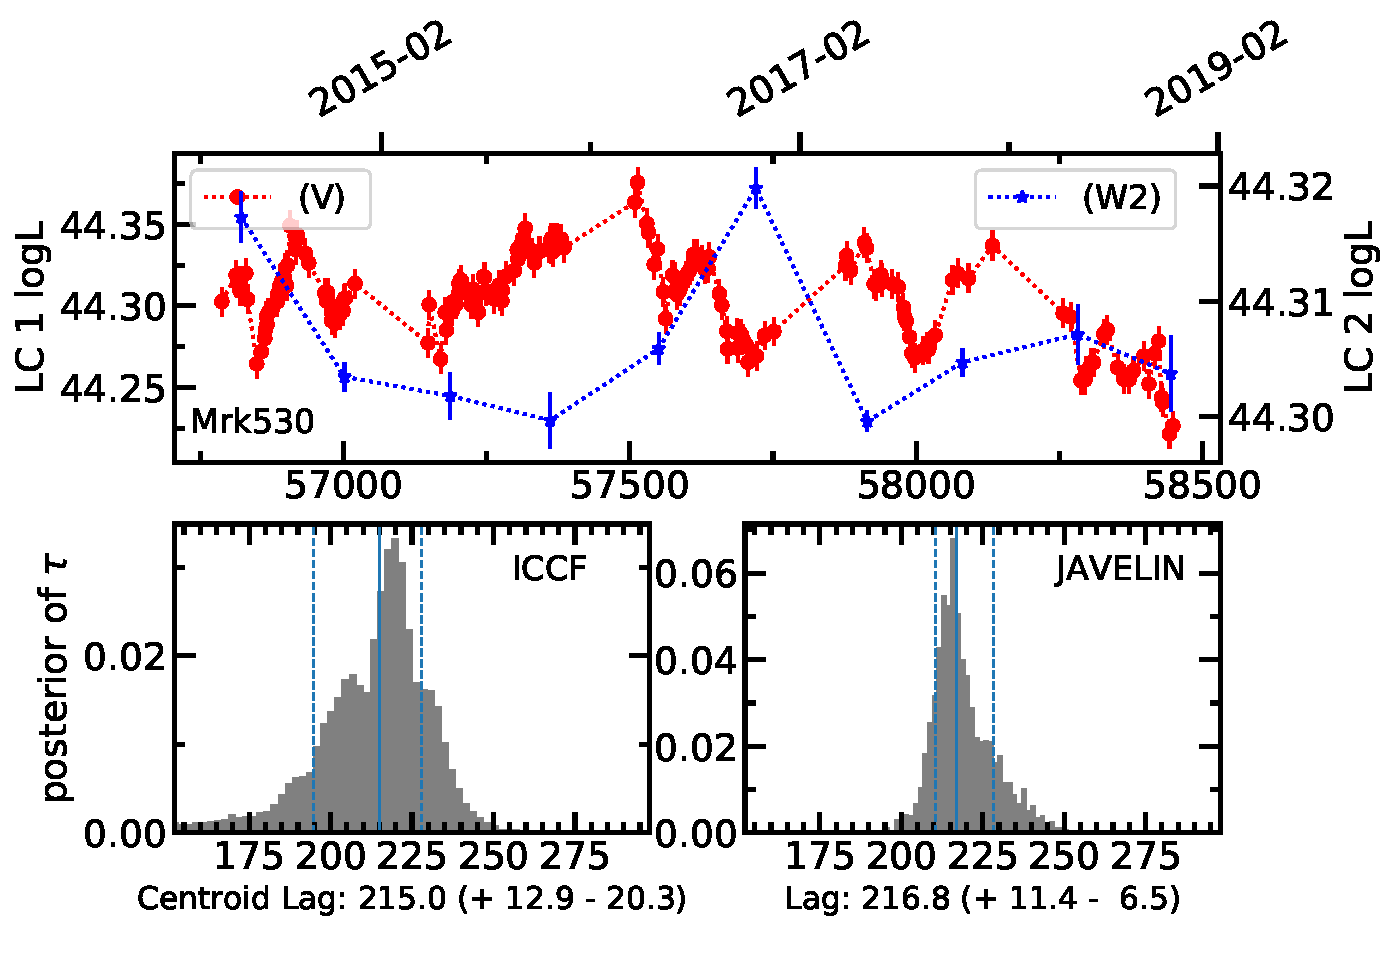
\includegraphics[width=0.45\textwidth]{pic/lag_pic/Mrk530_lag_w2.pdf} \\
    };
\end{tikzpicture}
%\label{fig:lag_clagn0}
%\caption{Dust-reverberation time lag analysis for CLAGNs.}
\end{figure}  

\begin{figure}[h!]
\begin{tikzpicture}
    \matrix[matrix of nodes]{
    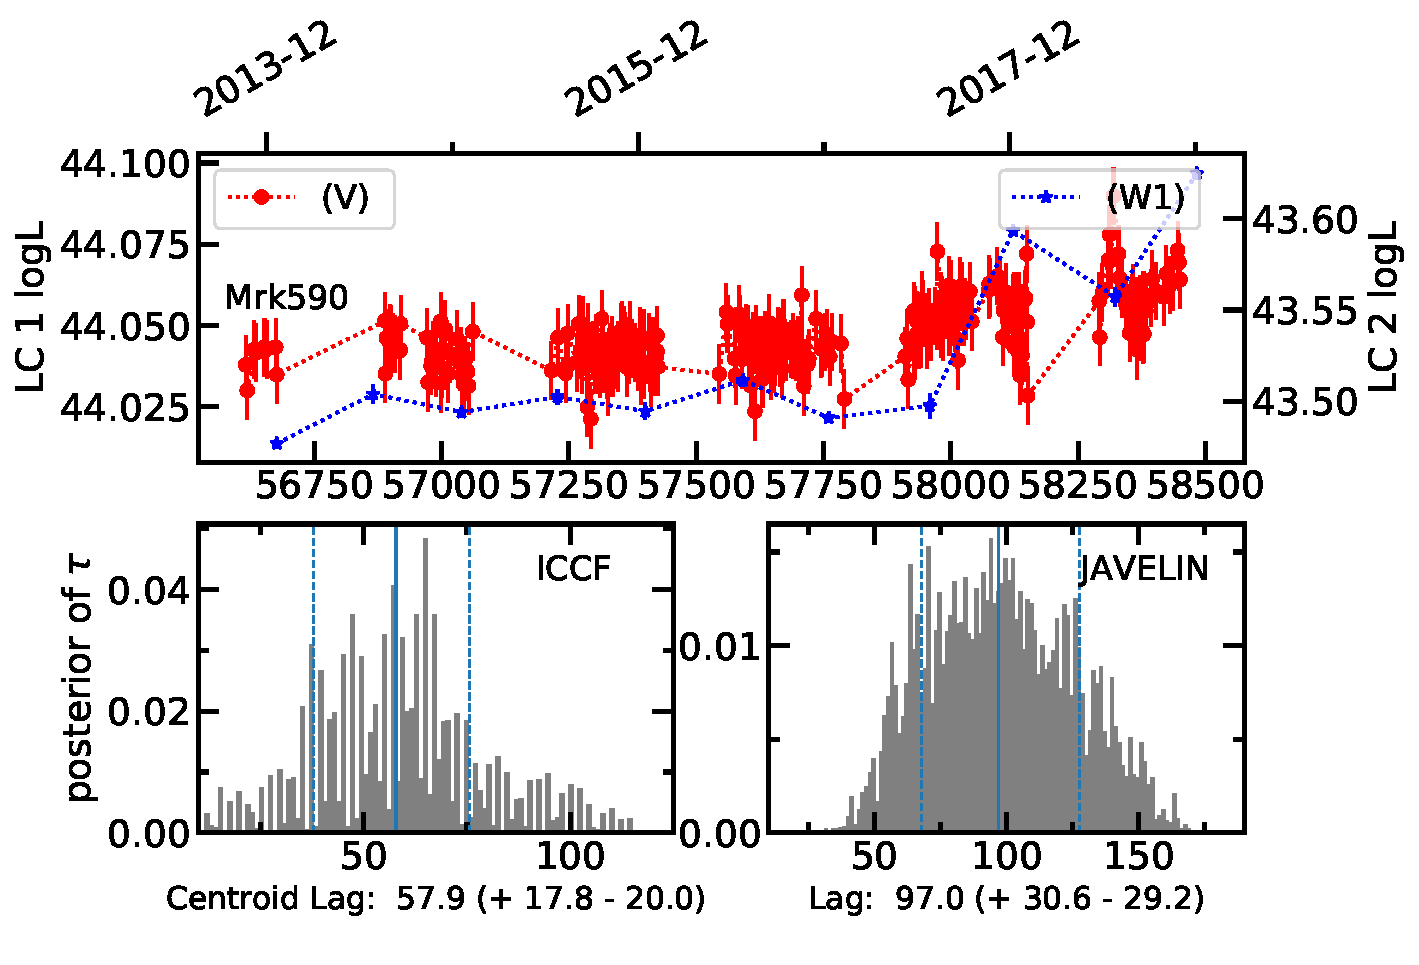
\includegraphics[width=0.45\textwidth]{pic/lag_pic/Mrk590lag.pdf}& \hspace{1em}  &
    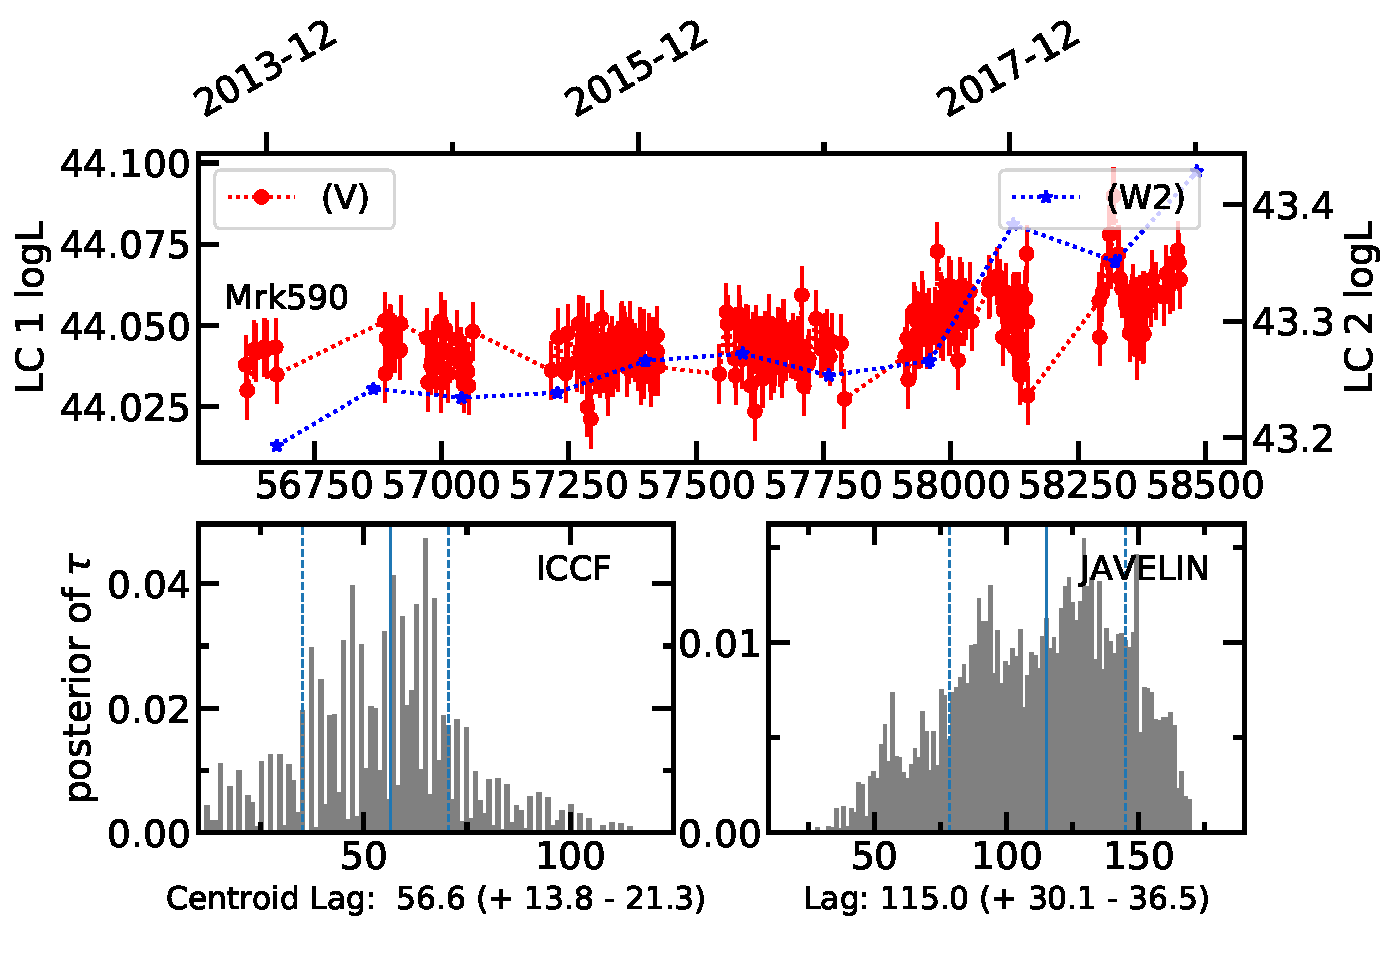
\includegraphics[width=0.45\textwidth]{pic/lag_pic/Mrk590lag_w2.pdf} \\
    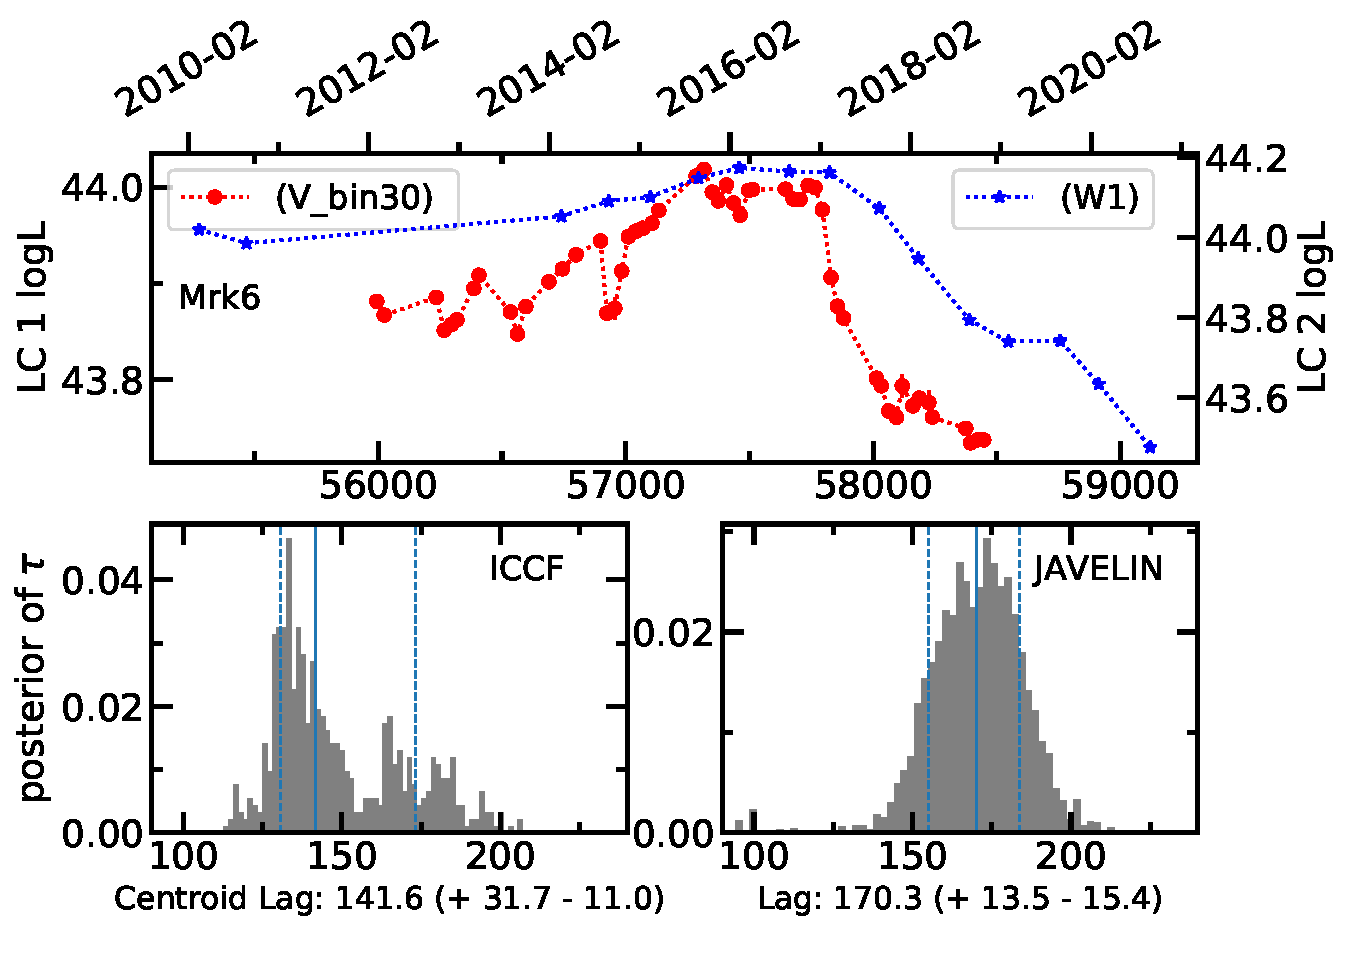
\includegraphics[width=0.45\textwidth]{pic/lag_pic/Mrk6lag1.pdf}& \hspace{1em}  &
    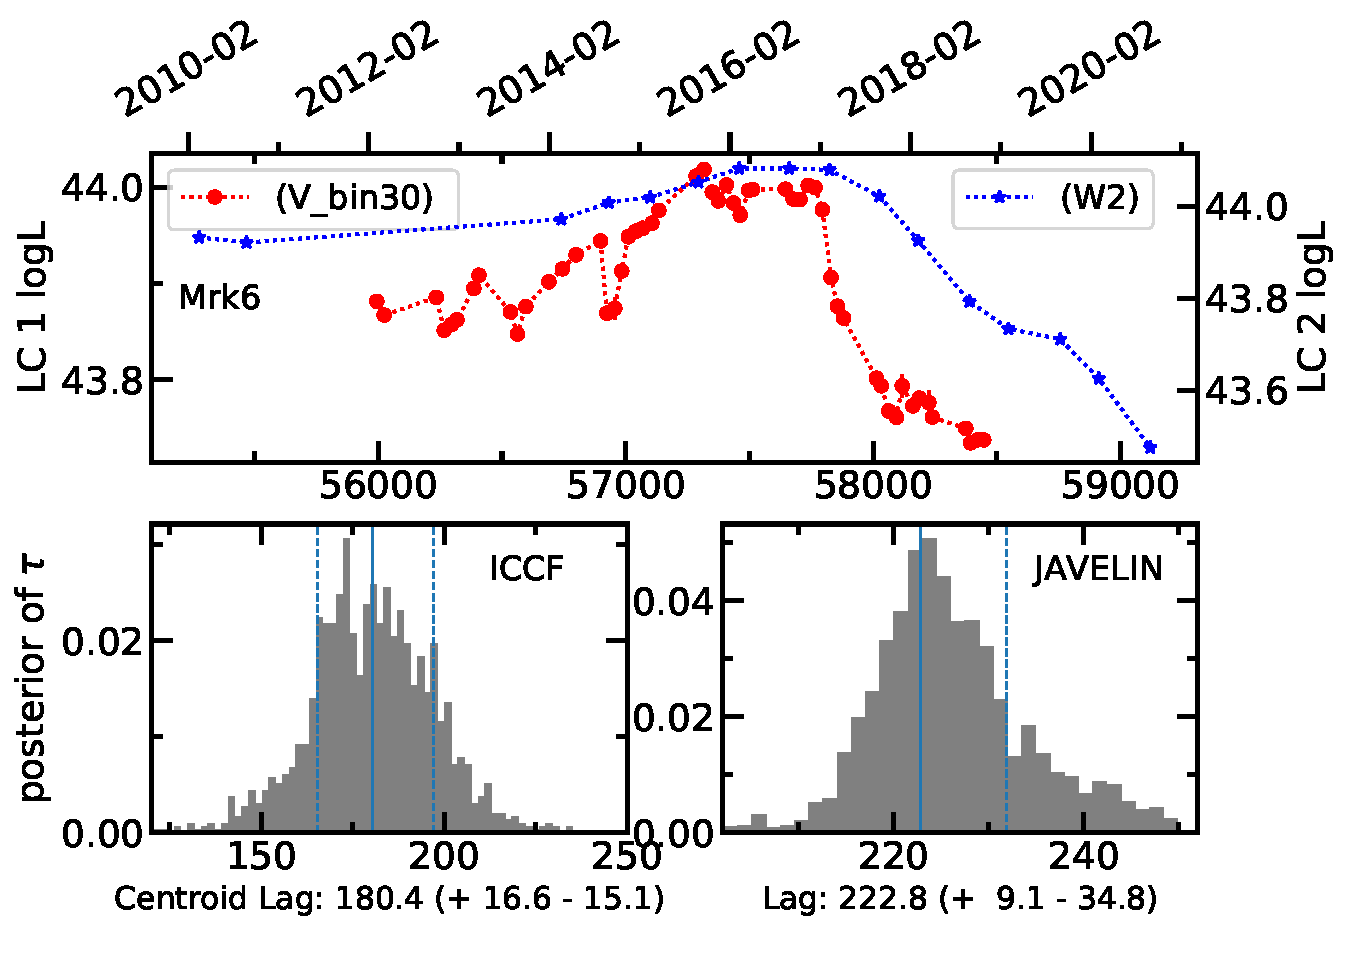
\includegraphics[width=0.45\textwidth]{pic/lag_pic/Mrk6lag1_w2.pdf} \\
    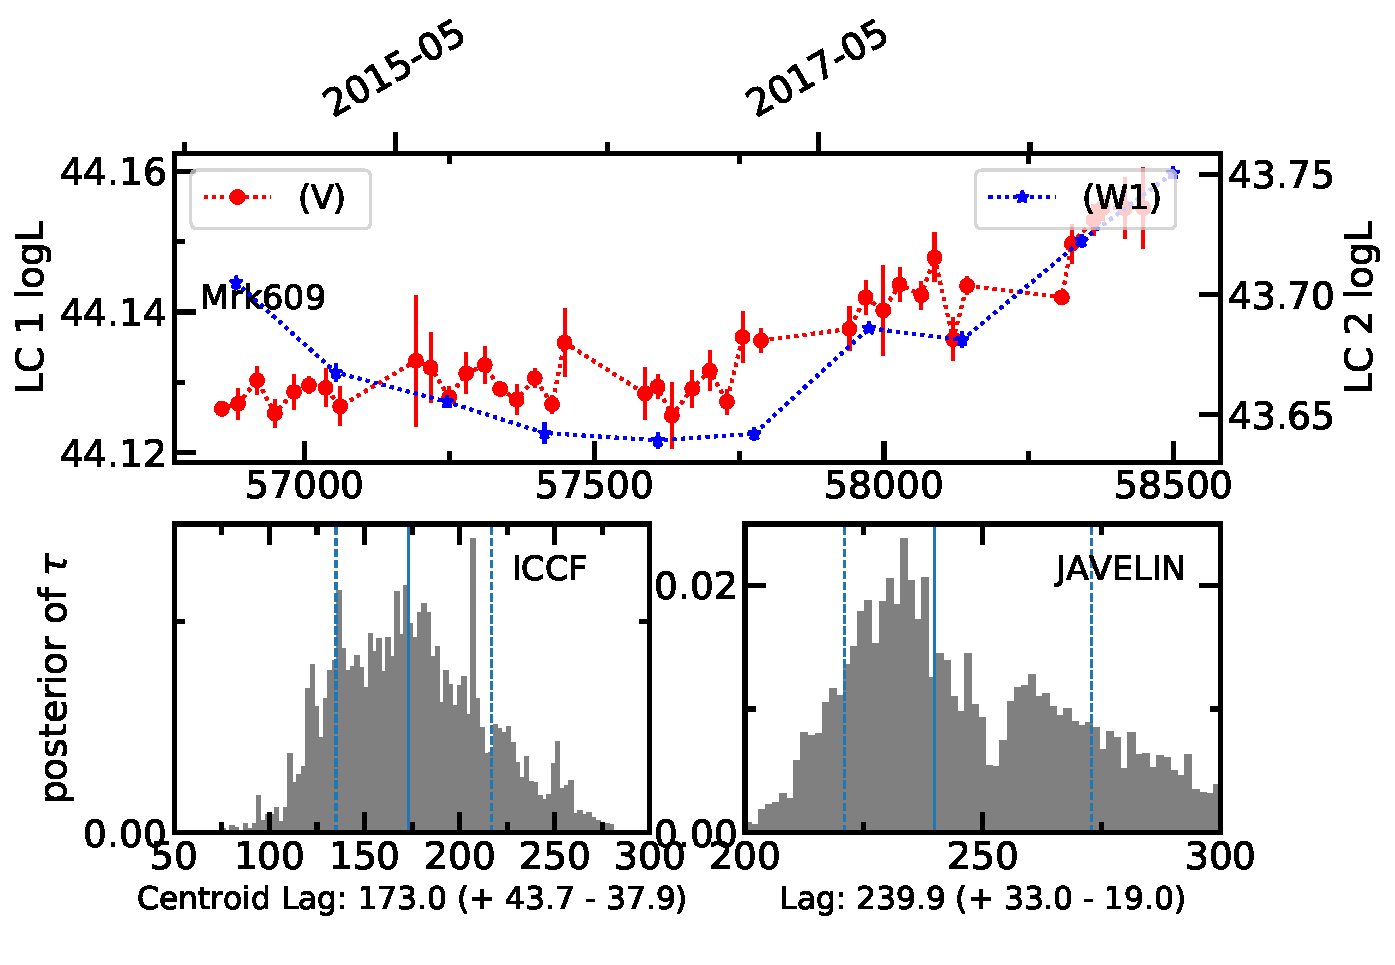
\includegraphics[width=0.45\textwidth]{pic/lag_pic/Mrk609lag1.pdf}& \hspace{1em}  &
    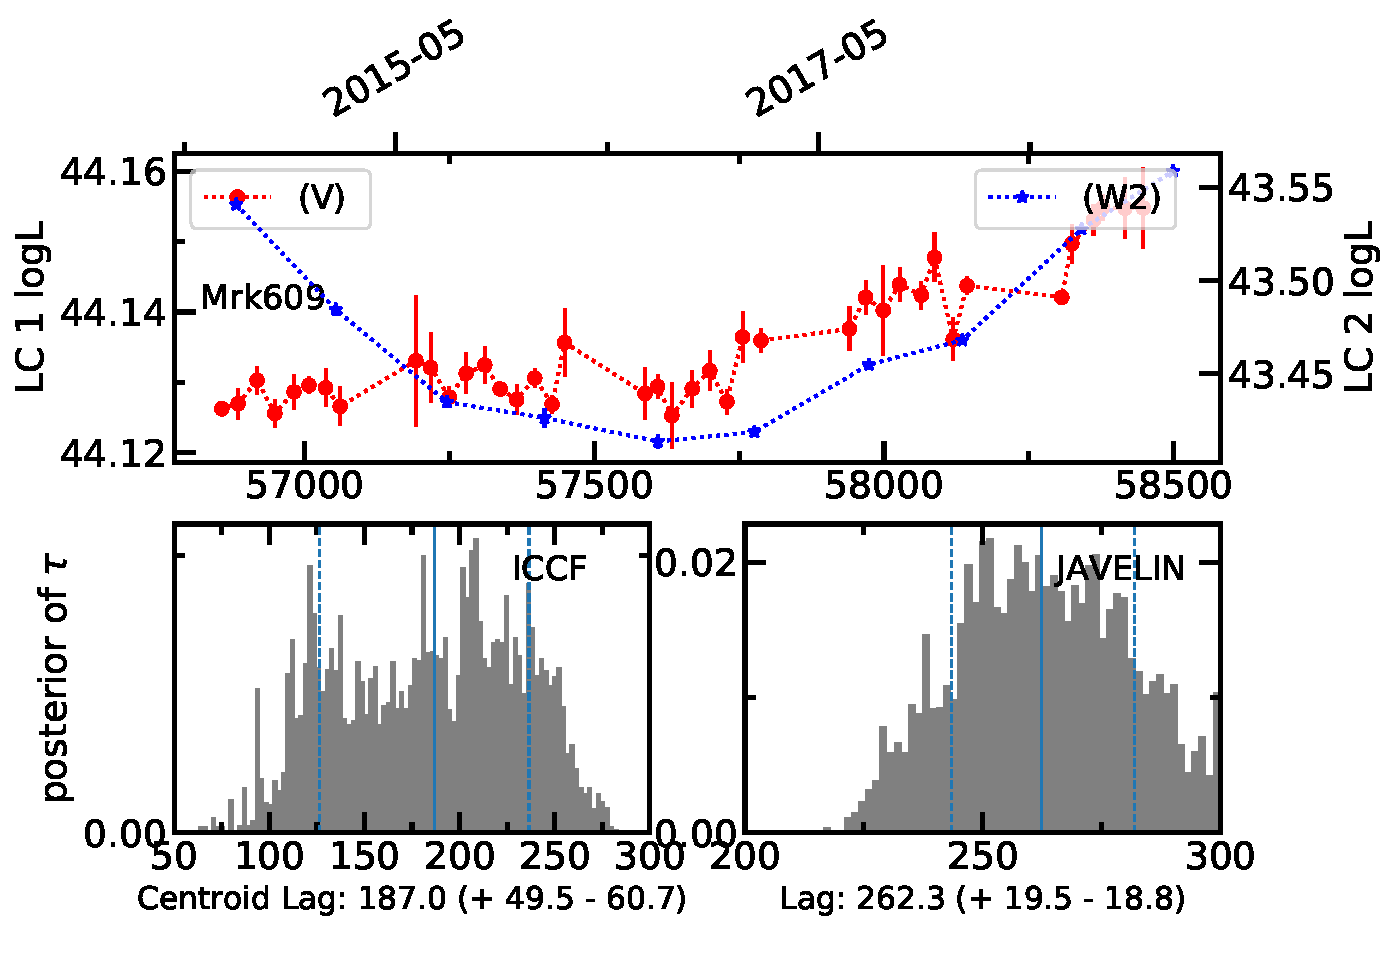
\includegraphics[width=0.45\textwidth]{pic/lag_pic/Mrk609lag1_w2.pdf} \\    
    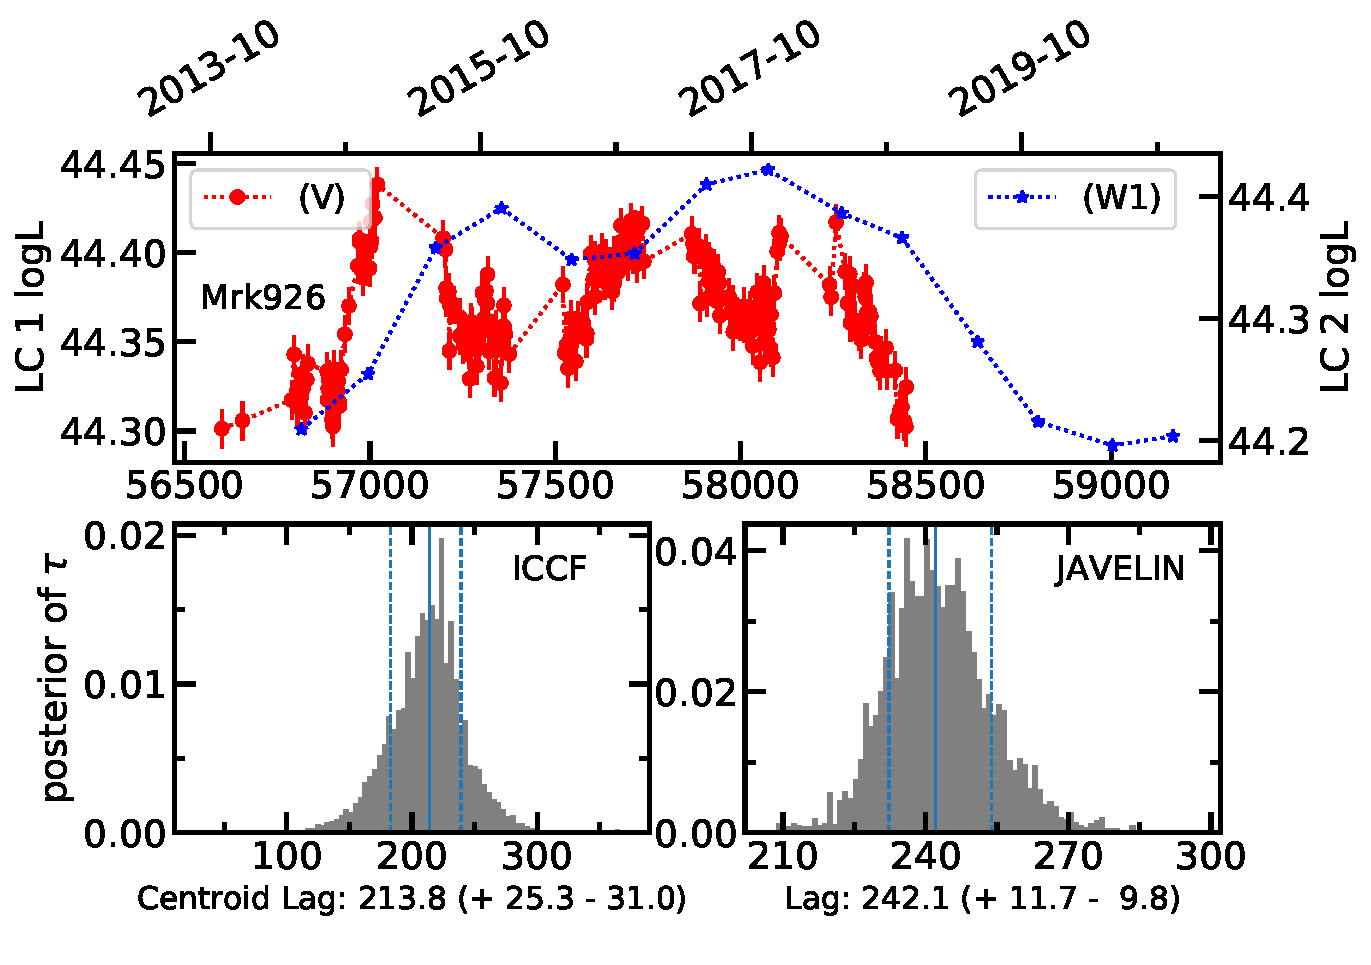
\includegraphics[width=0.45\textwidth]{pic/lag_pic/Mrk926lag.pdf}& \hspace{1em}  &
    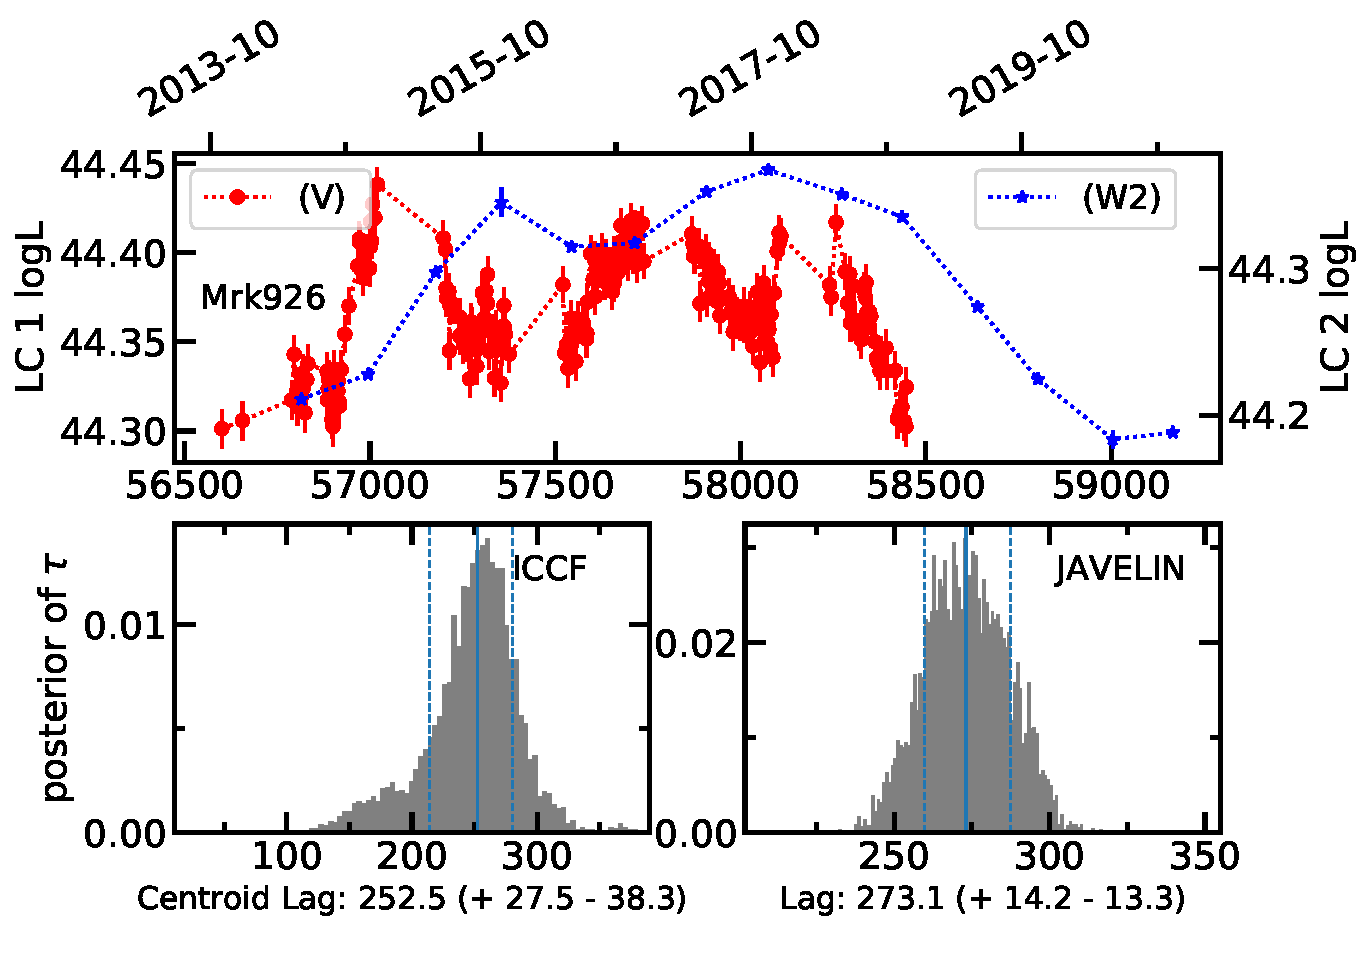
\includegraphics[width=0.45\textwidth]{pic/lag_pic/Mrk926lag_w2.pdf} \\
    };
\end{tikzpicture}
%\label{fig:lag_clagn0}
%\caption{Dust-reverberation time lag analysis for CLAGNs.}
\end{figure}  
\begin{figure}[h!]
\begin{tikzpicture}
    \matrix[matrix of nodes]{
    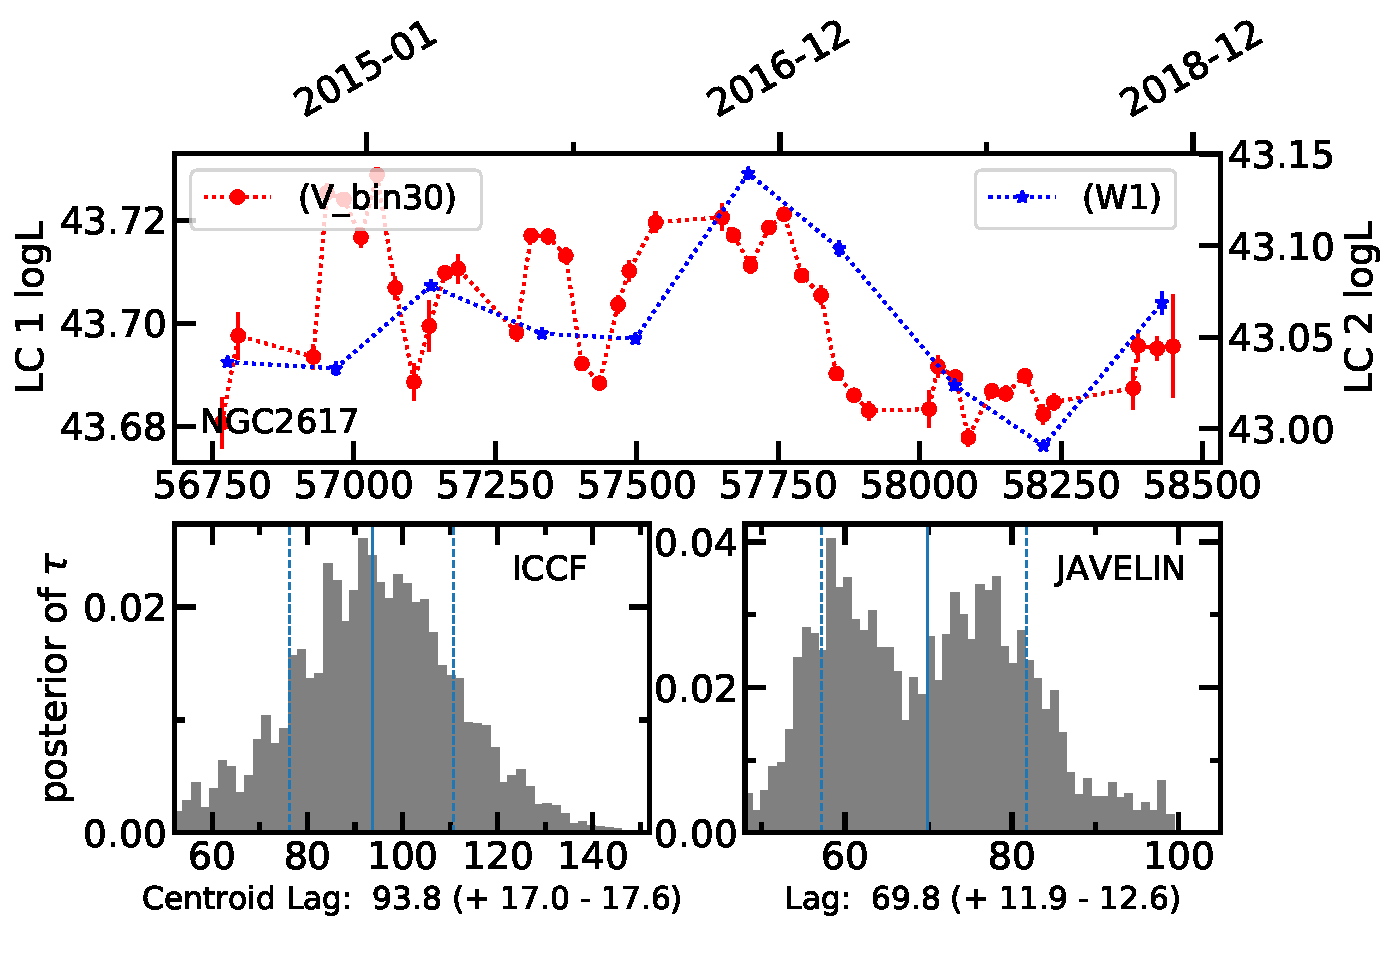
\includegraphics[width=0.45\textwidth]{pic/lag_pic/NGC2617lag1.pdf}& \hspace{1em}  &
    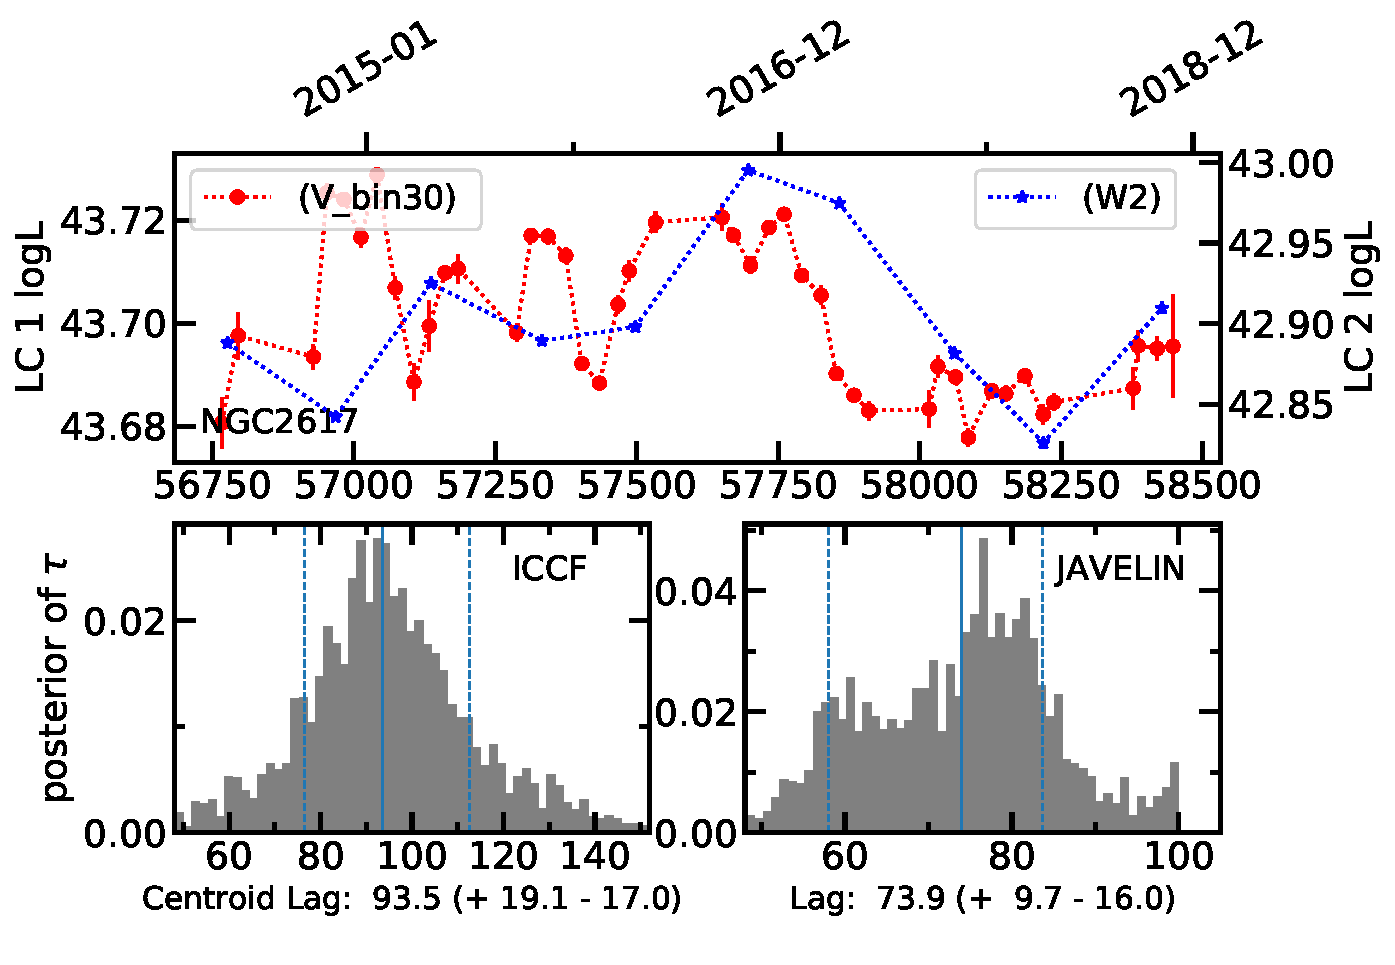
\includegraphics[width=0.45\textwidth]{pic/lag_pic/NGC2617lag1_w2.pdf} \\   
    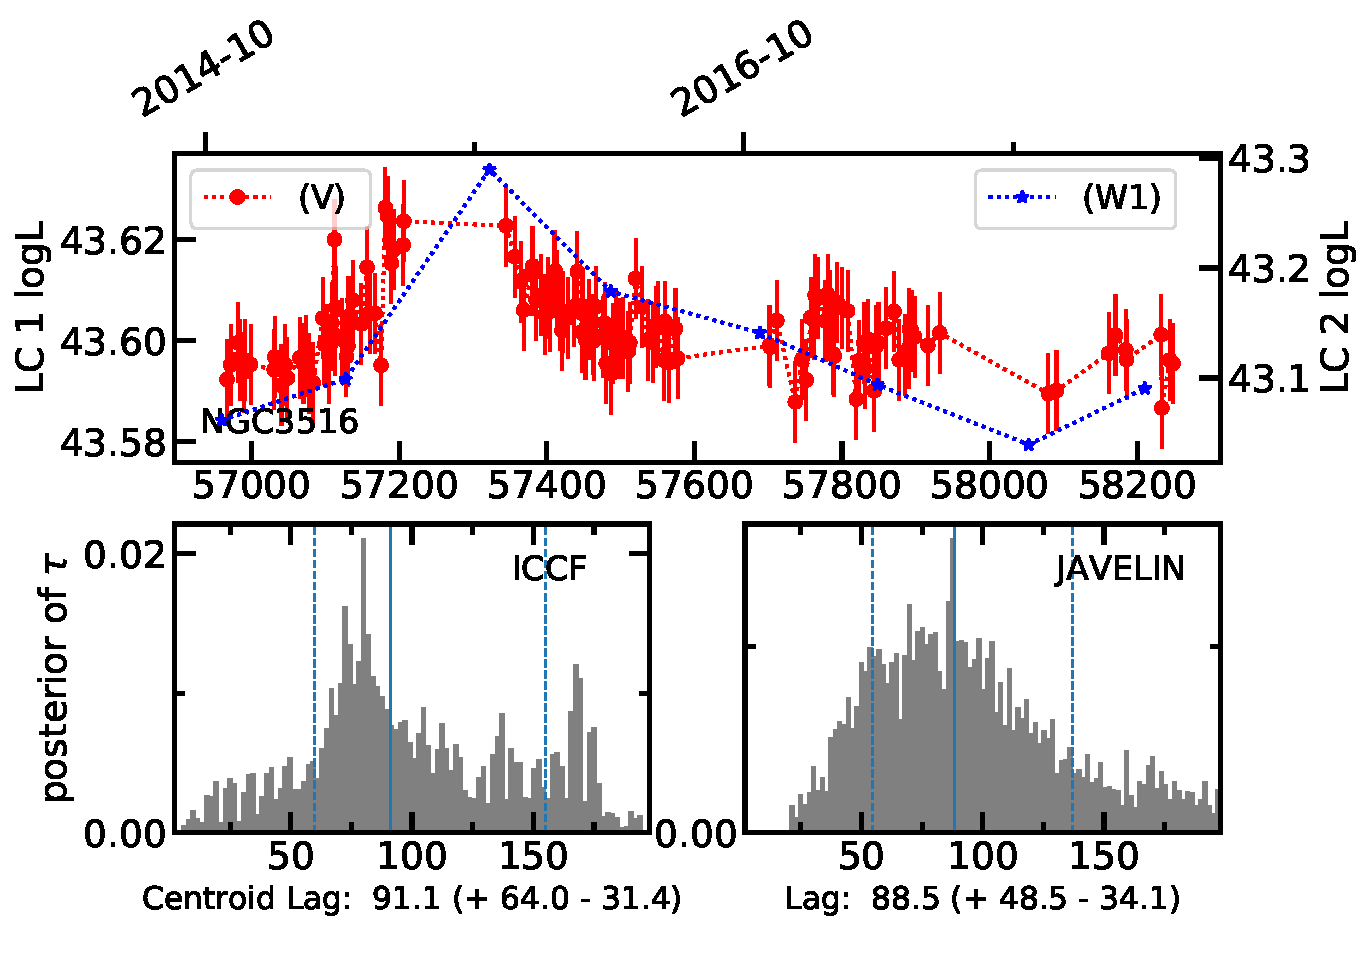
\includegraphics[width=0.45\textwidth]{pic/lag_pic/NGC3516lag.pdf}& \hspace{1em}  &
    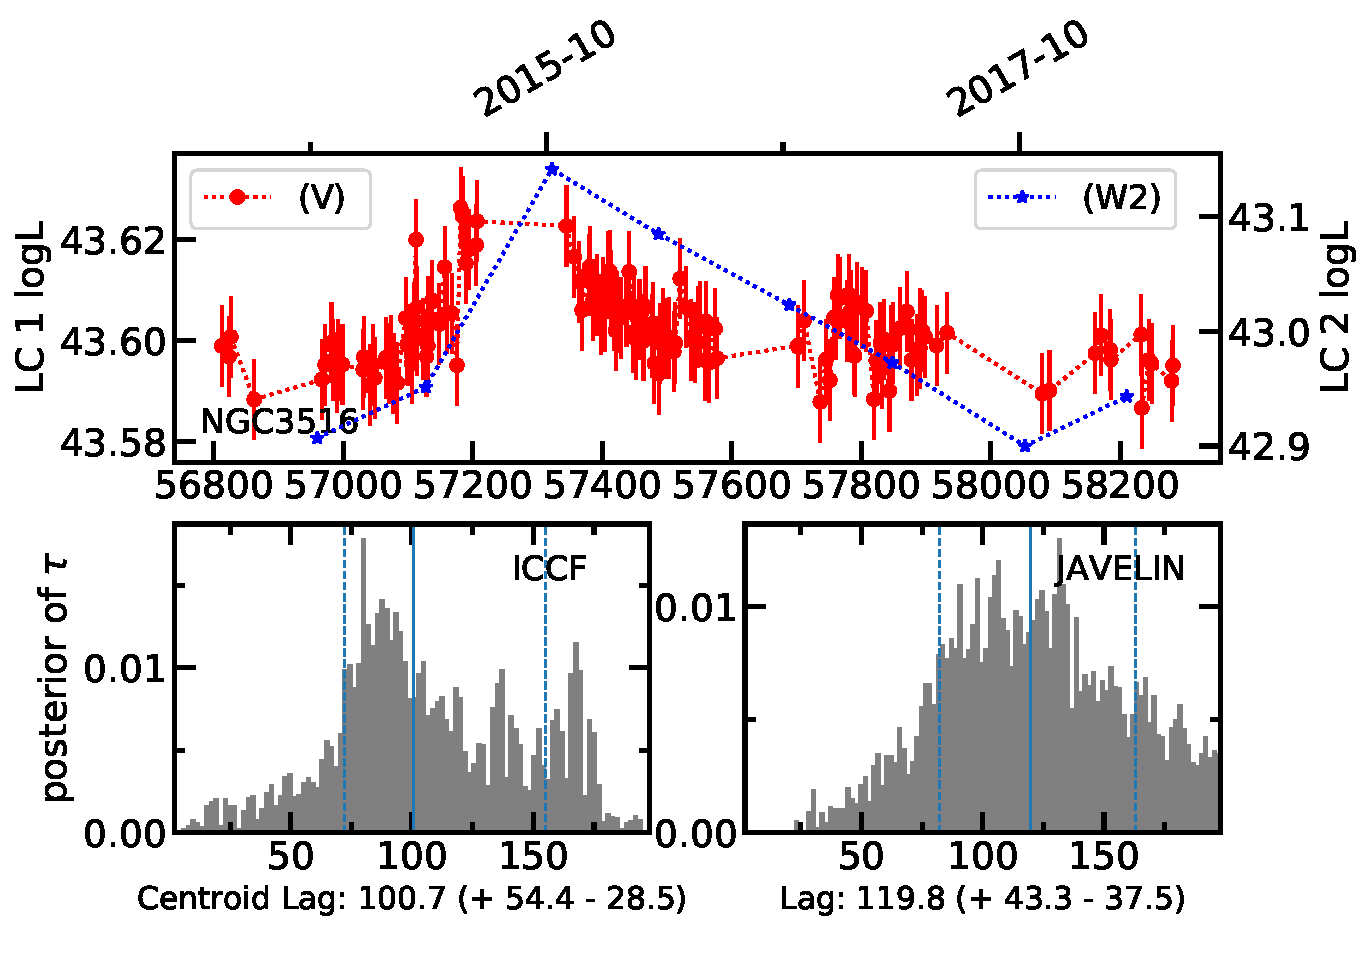
\includegraphics[width=0.45\textwidth]{pic/lag_pic/NGC3516lag_w2.pdf} \\
    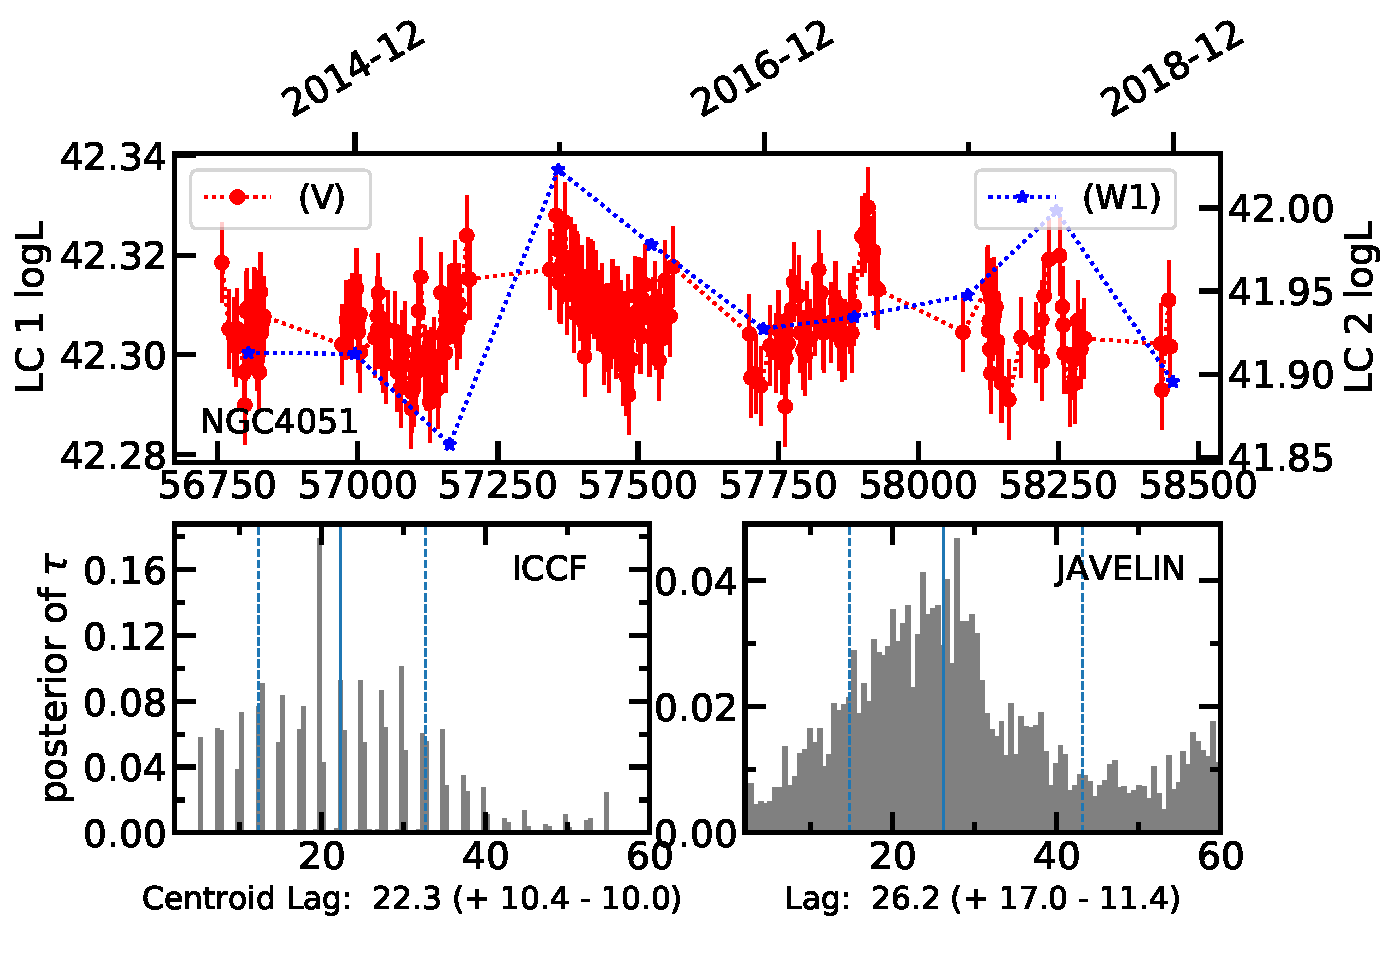
\includegraphics[width=0.45\textwidth]{pic/lag_pic/NGC4051lag.pdf}& \hspace{1em}  &
    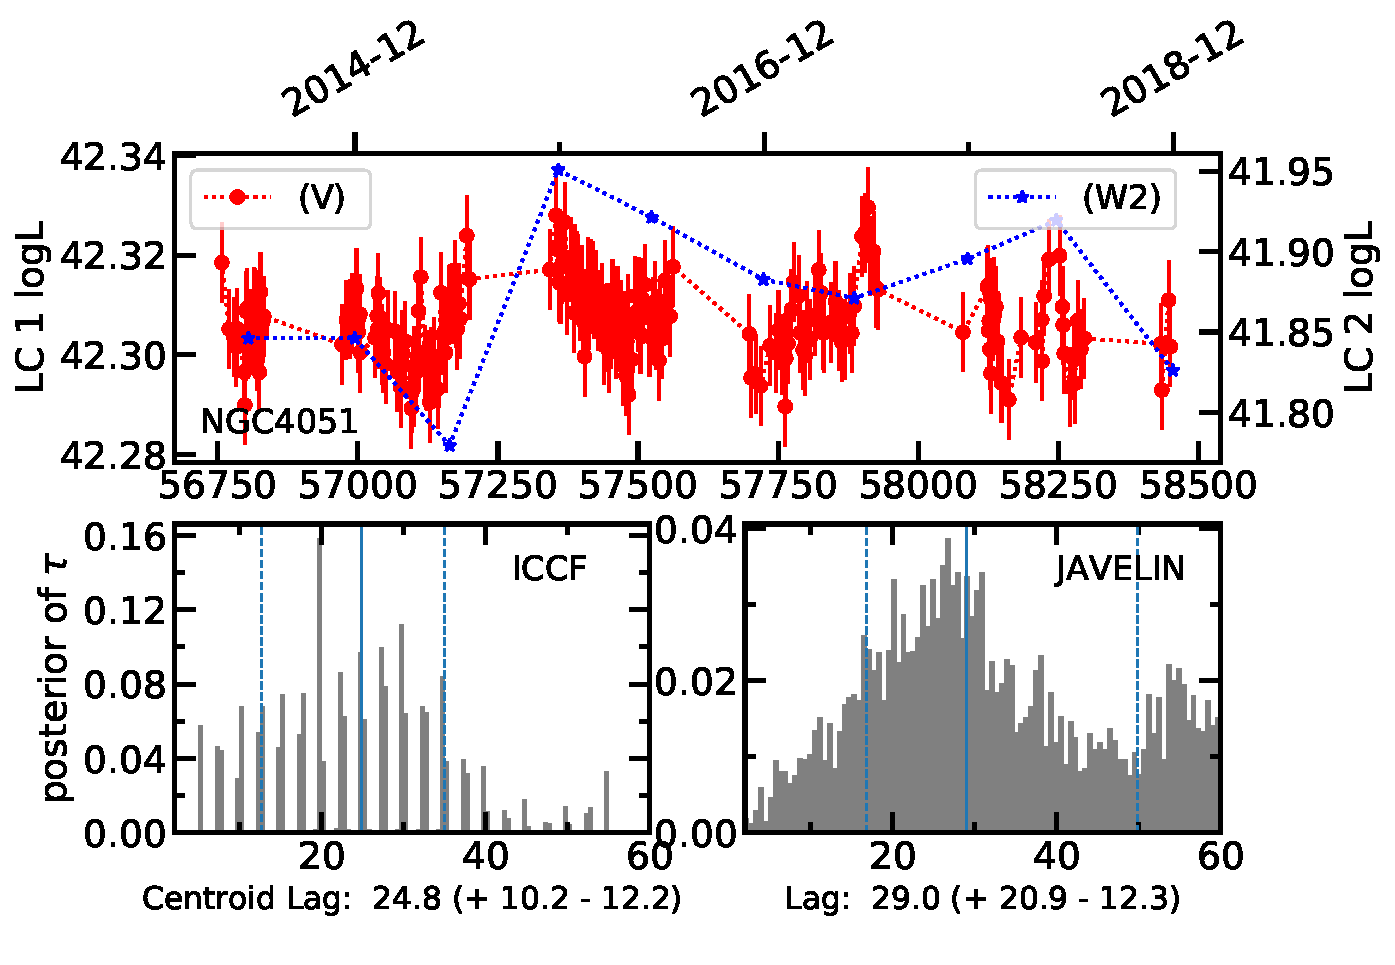
\includegraphics[width=0.45\textwidth]{pic/lag_pic/NGC4051lag_w2.pdf} \\
    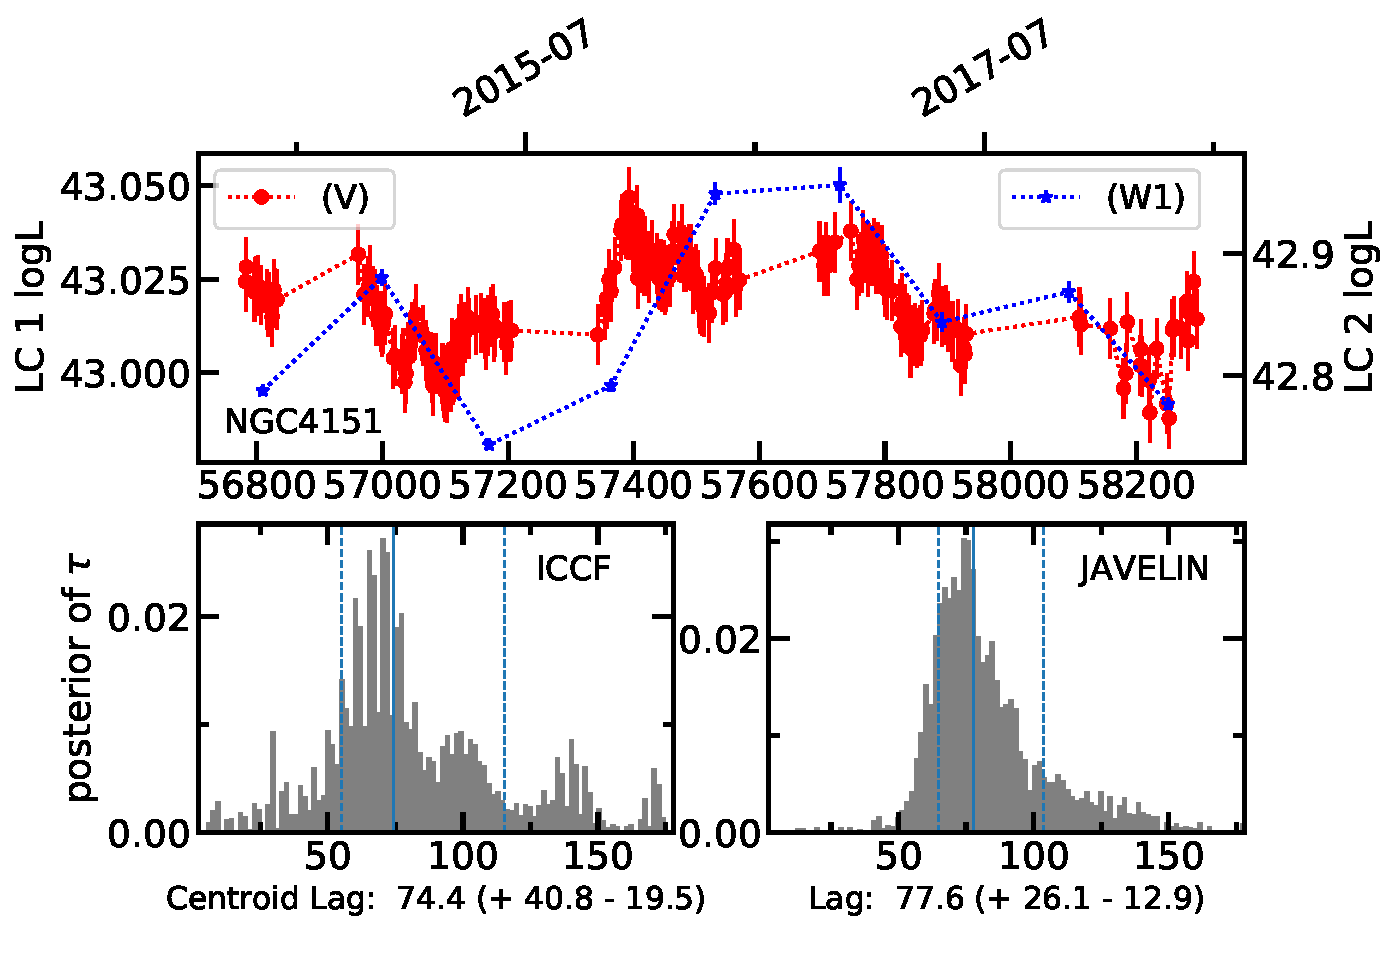
\includegraphics[width=0.45\textwidth]{pic/lag_pic/NGC4151lag.pdf}& \hspace{1em}  &
    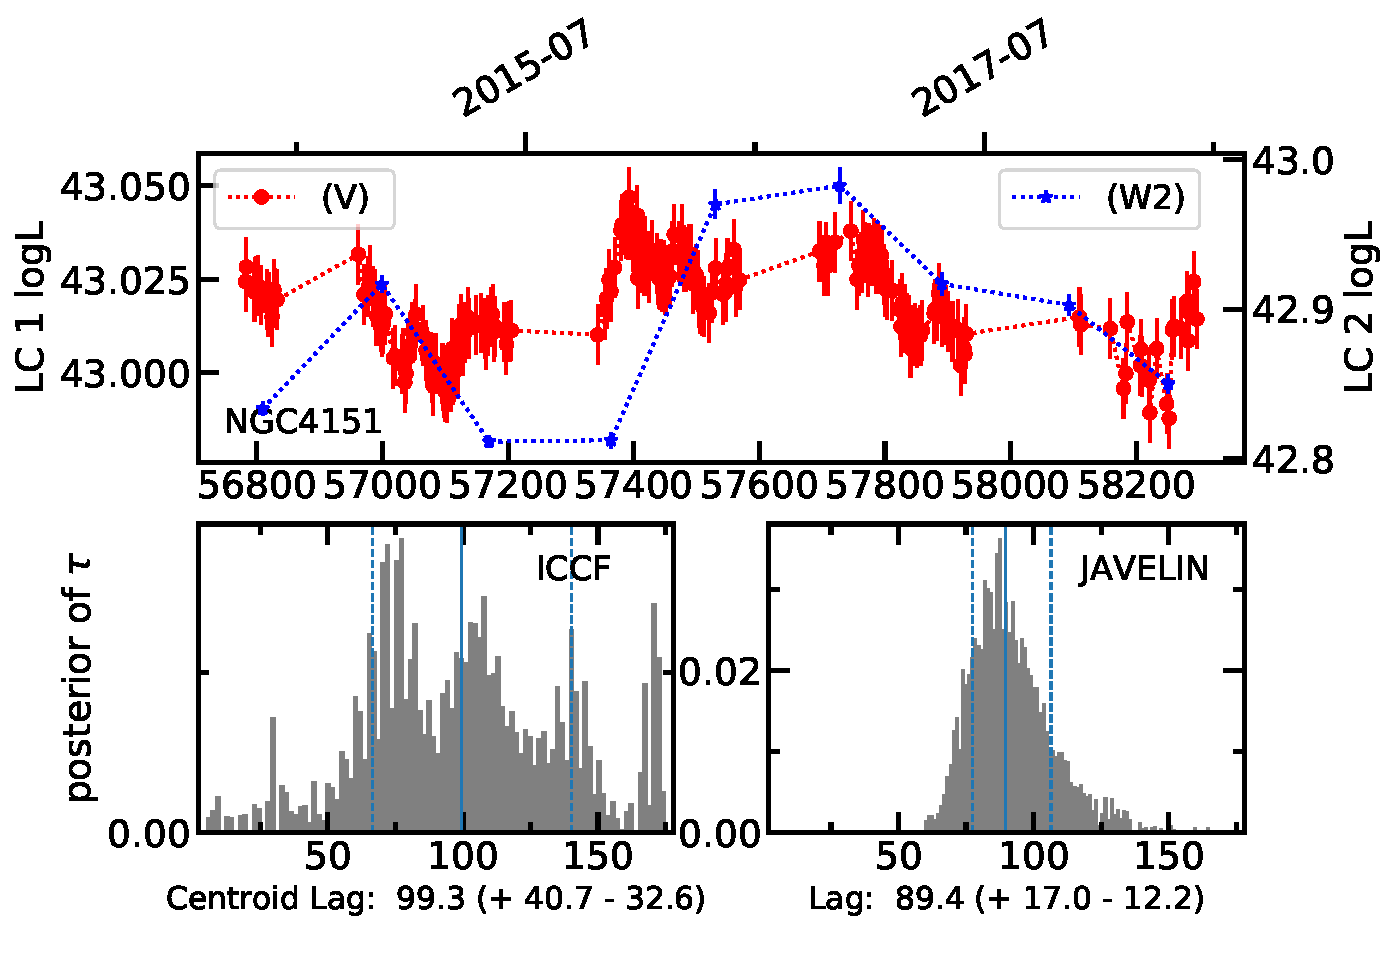
\includegraphics[width=0.45\textwidth]{pic/lag_pic/NGC4151lag_w2.pdf} \\
    };
\end{tikzpicture}
%\label{fig:lag_clagn1}
%\caption{Dust-reverberation time lag analysis for CLAGNs.}
\end{figure}  


\begin{figure}[h!]
\begin{tikzpicture}
    \matrix[matrix of nodes]{
    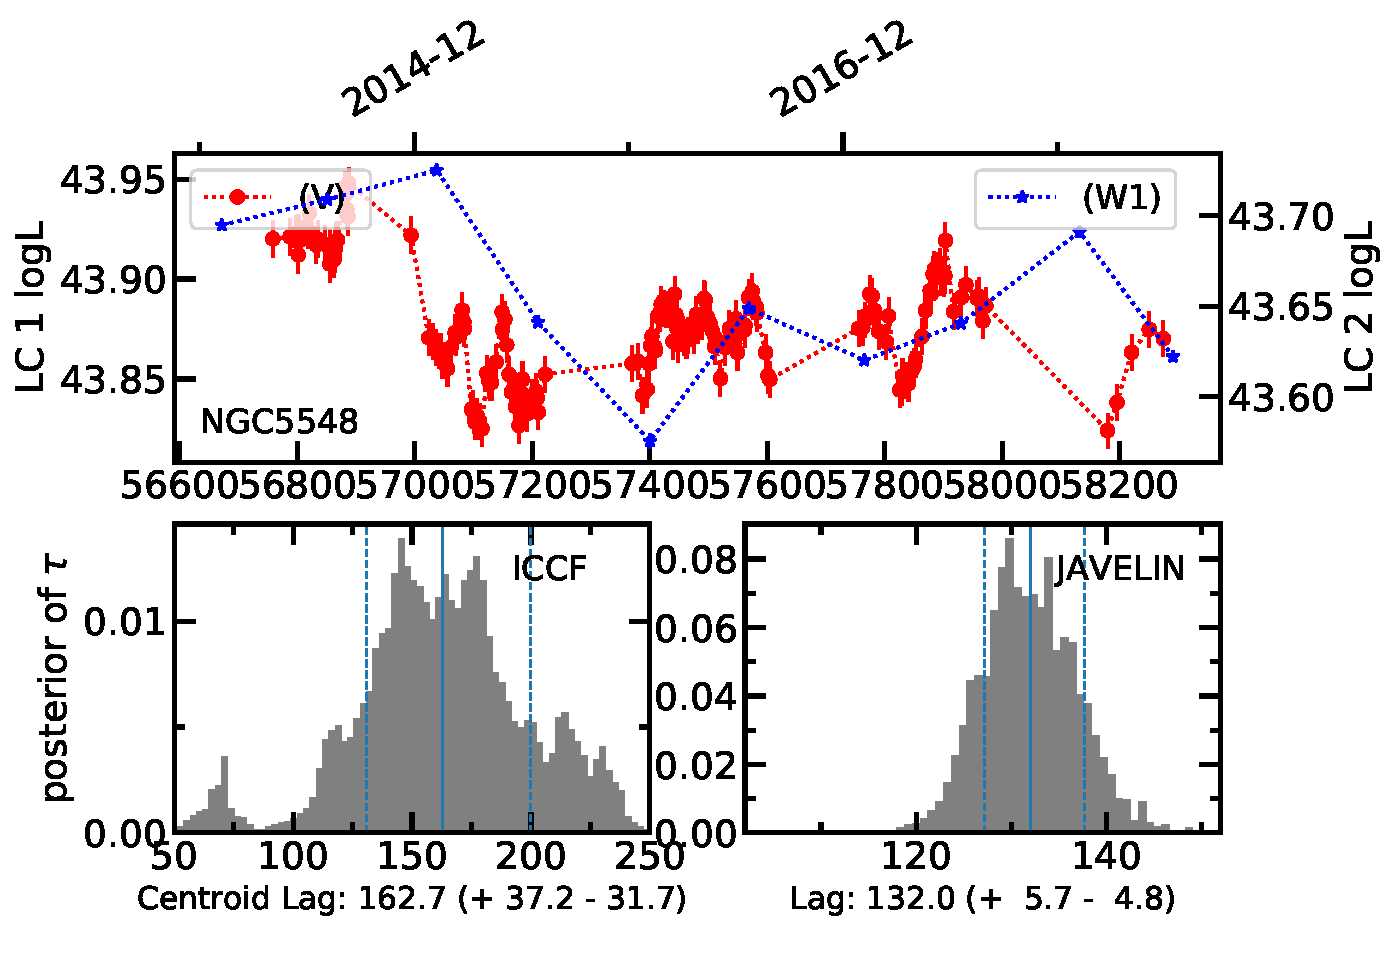
\includegraphics[width=0.45\textwidth]{pic/lag_pic/NGC5548lag.pdf}& \hspace{1em}  &
    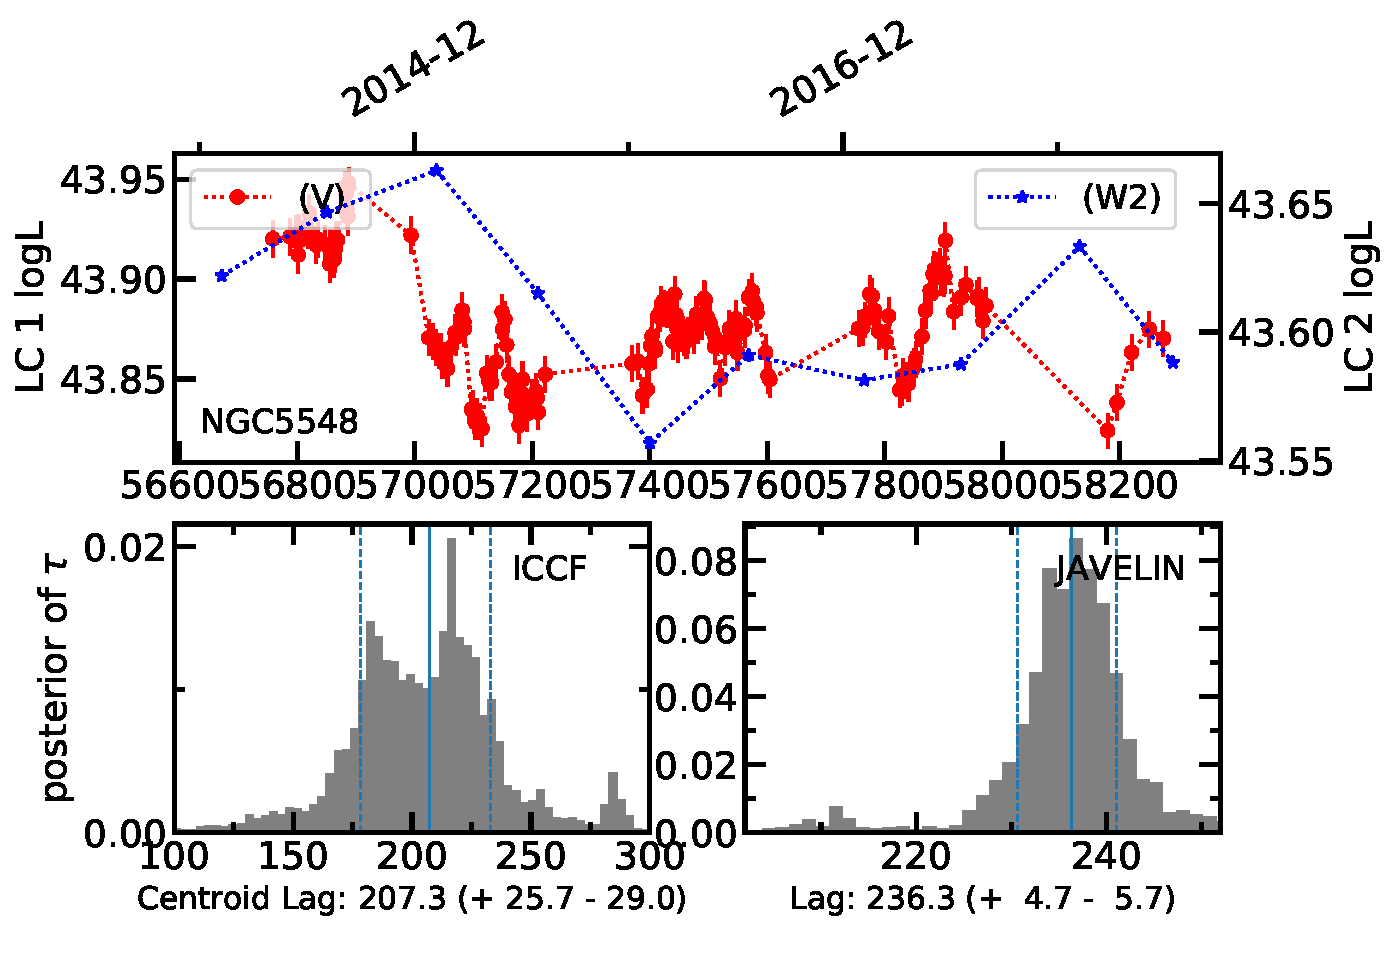
\includegraphics[width=0.45\textwidth]{pic/lag_pic/NGC5548lag_w2.pdf} \\    
    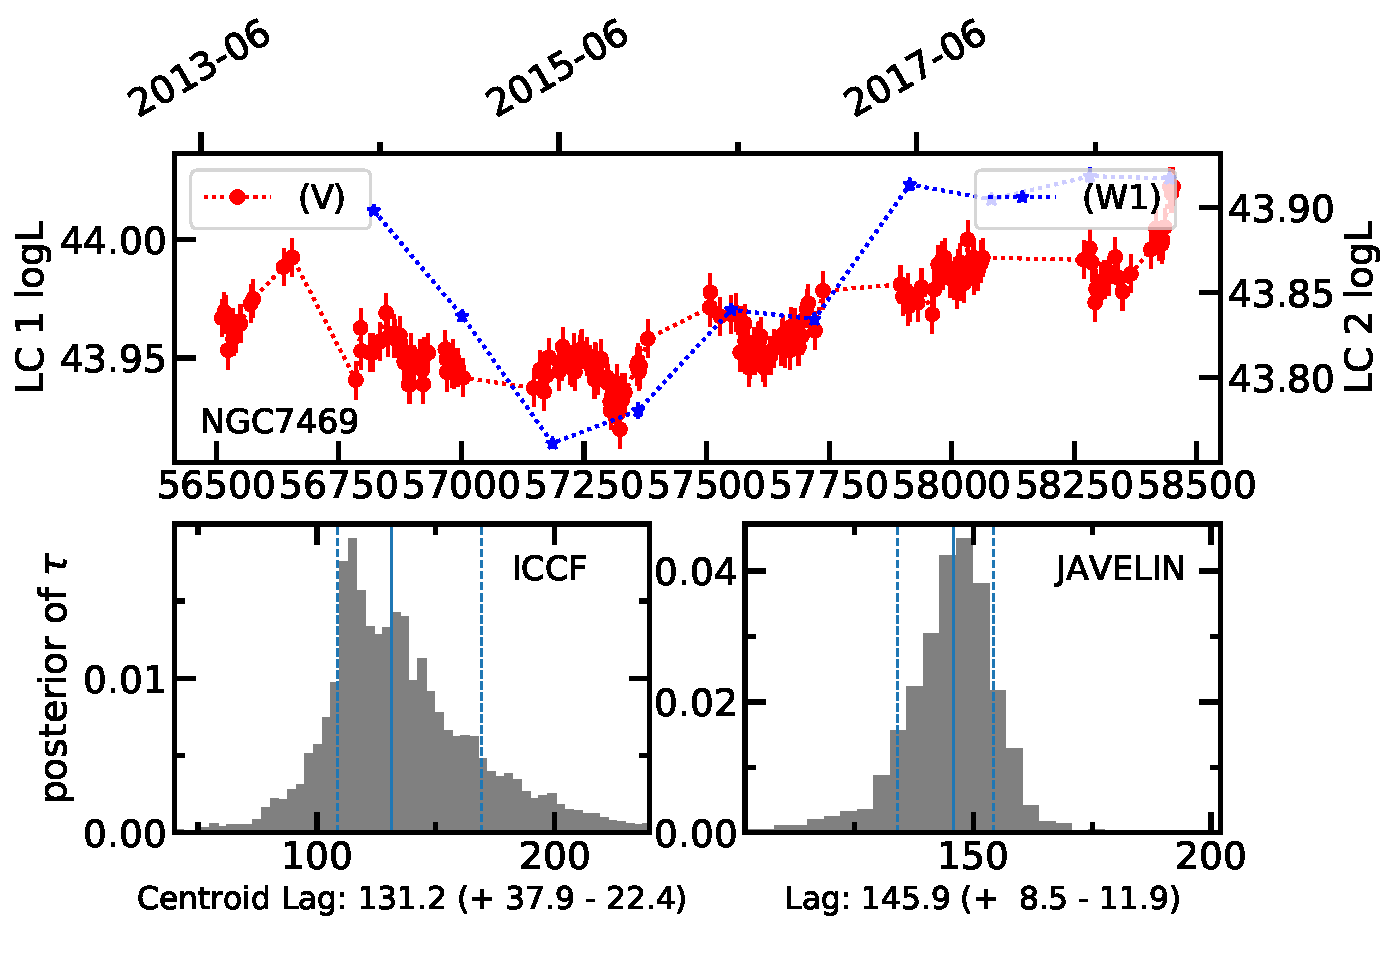
\includegraphics[width=0.45\textwidth]{pic/lag_pic/NGC7469lag.pdf}& \hspace{1em}  &
    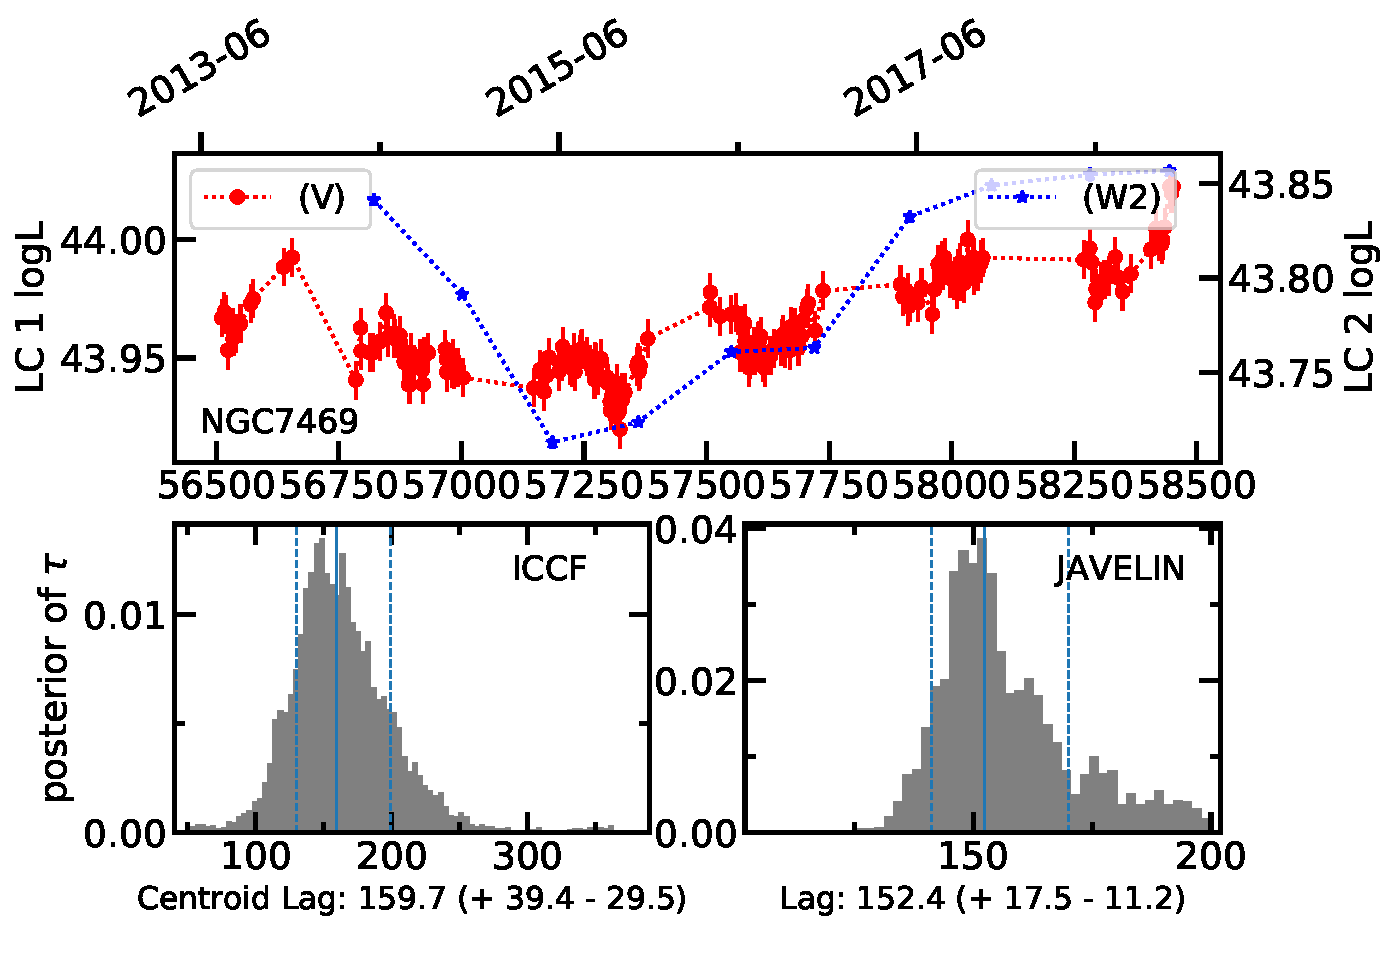
\includegraphics[width=0.45\textwidth]{pic/lag_pic/NGC7469lag_w2.pdf} \\
    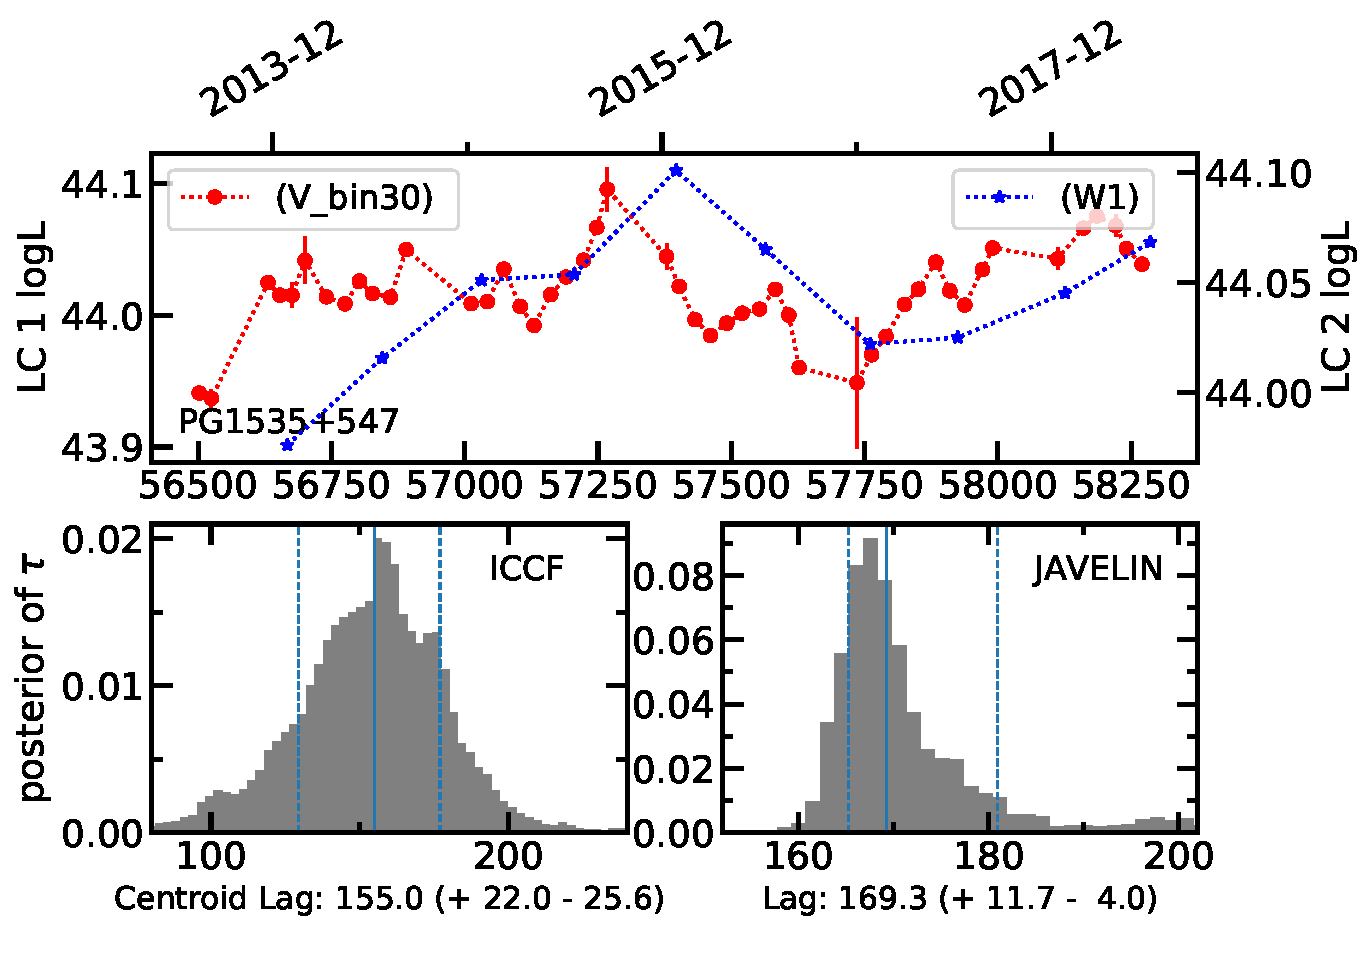
\includegraphics[width=0.45\textwidth]{pic/lag_pic/PG1535p547lag1.pdf}& \hspace{1em}  &
    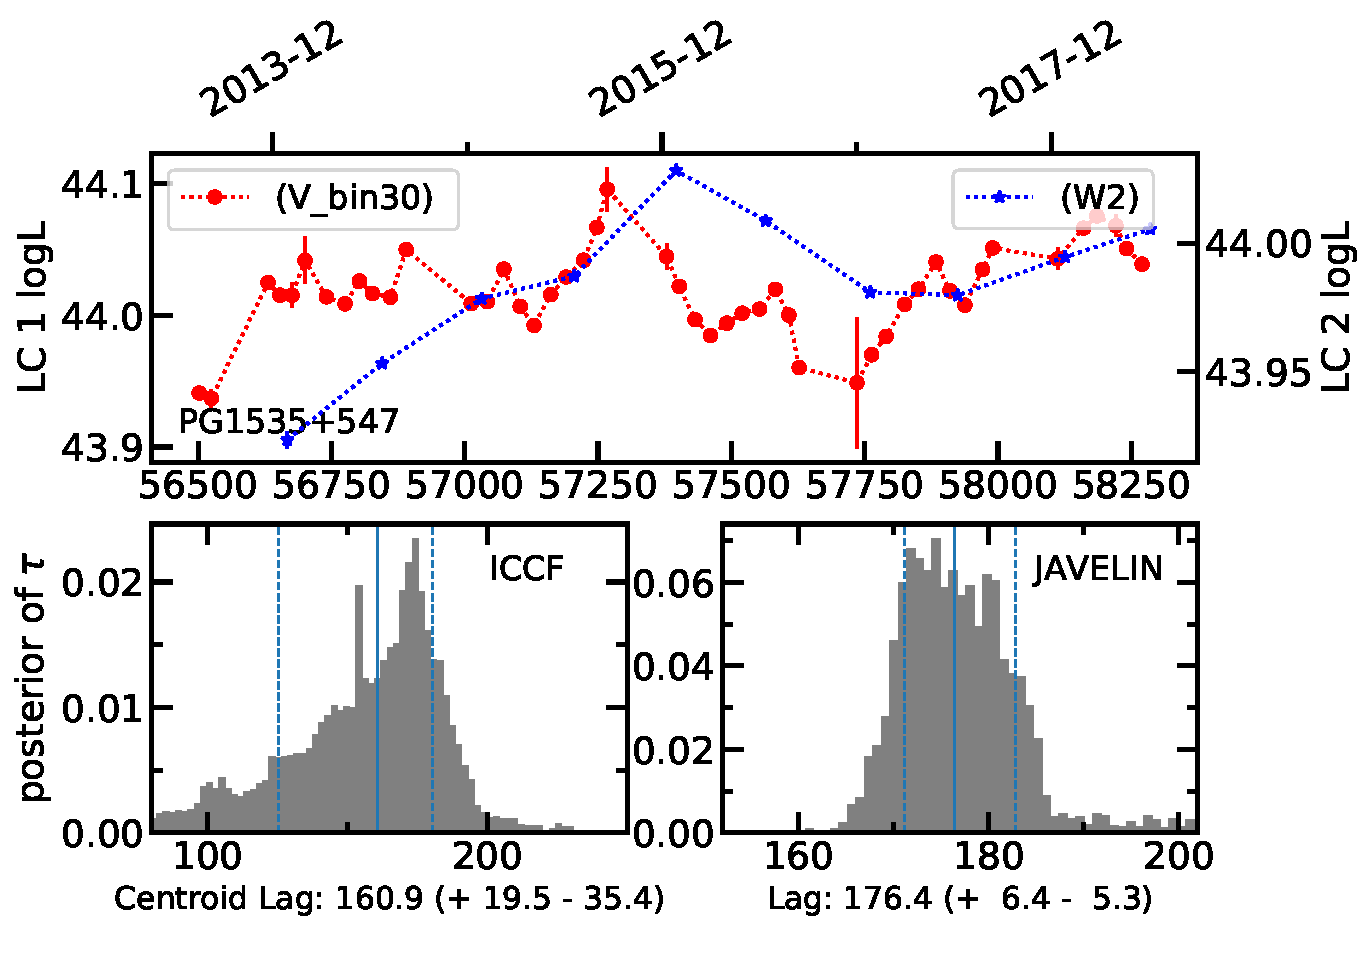
\includegraphics[width=0.45\textwidth]{pic/lag_pic/PG1535p547lag1_w2.pdf} \\   
    };
\end{tikzpicture}
%\label{fig:lag_clagn2}
\caption{Mid-IR dust reverberation mapping analysis results for CLAGNs.}
\end{figure}  
\end{document}

% End of file `sample631.tex'.



